% Created by tikzDevice version 0.10.1 on 2016-03-25 13:33:55
% !TEX encoding = UTF-8 Unicode
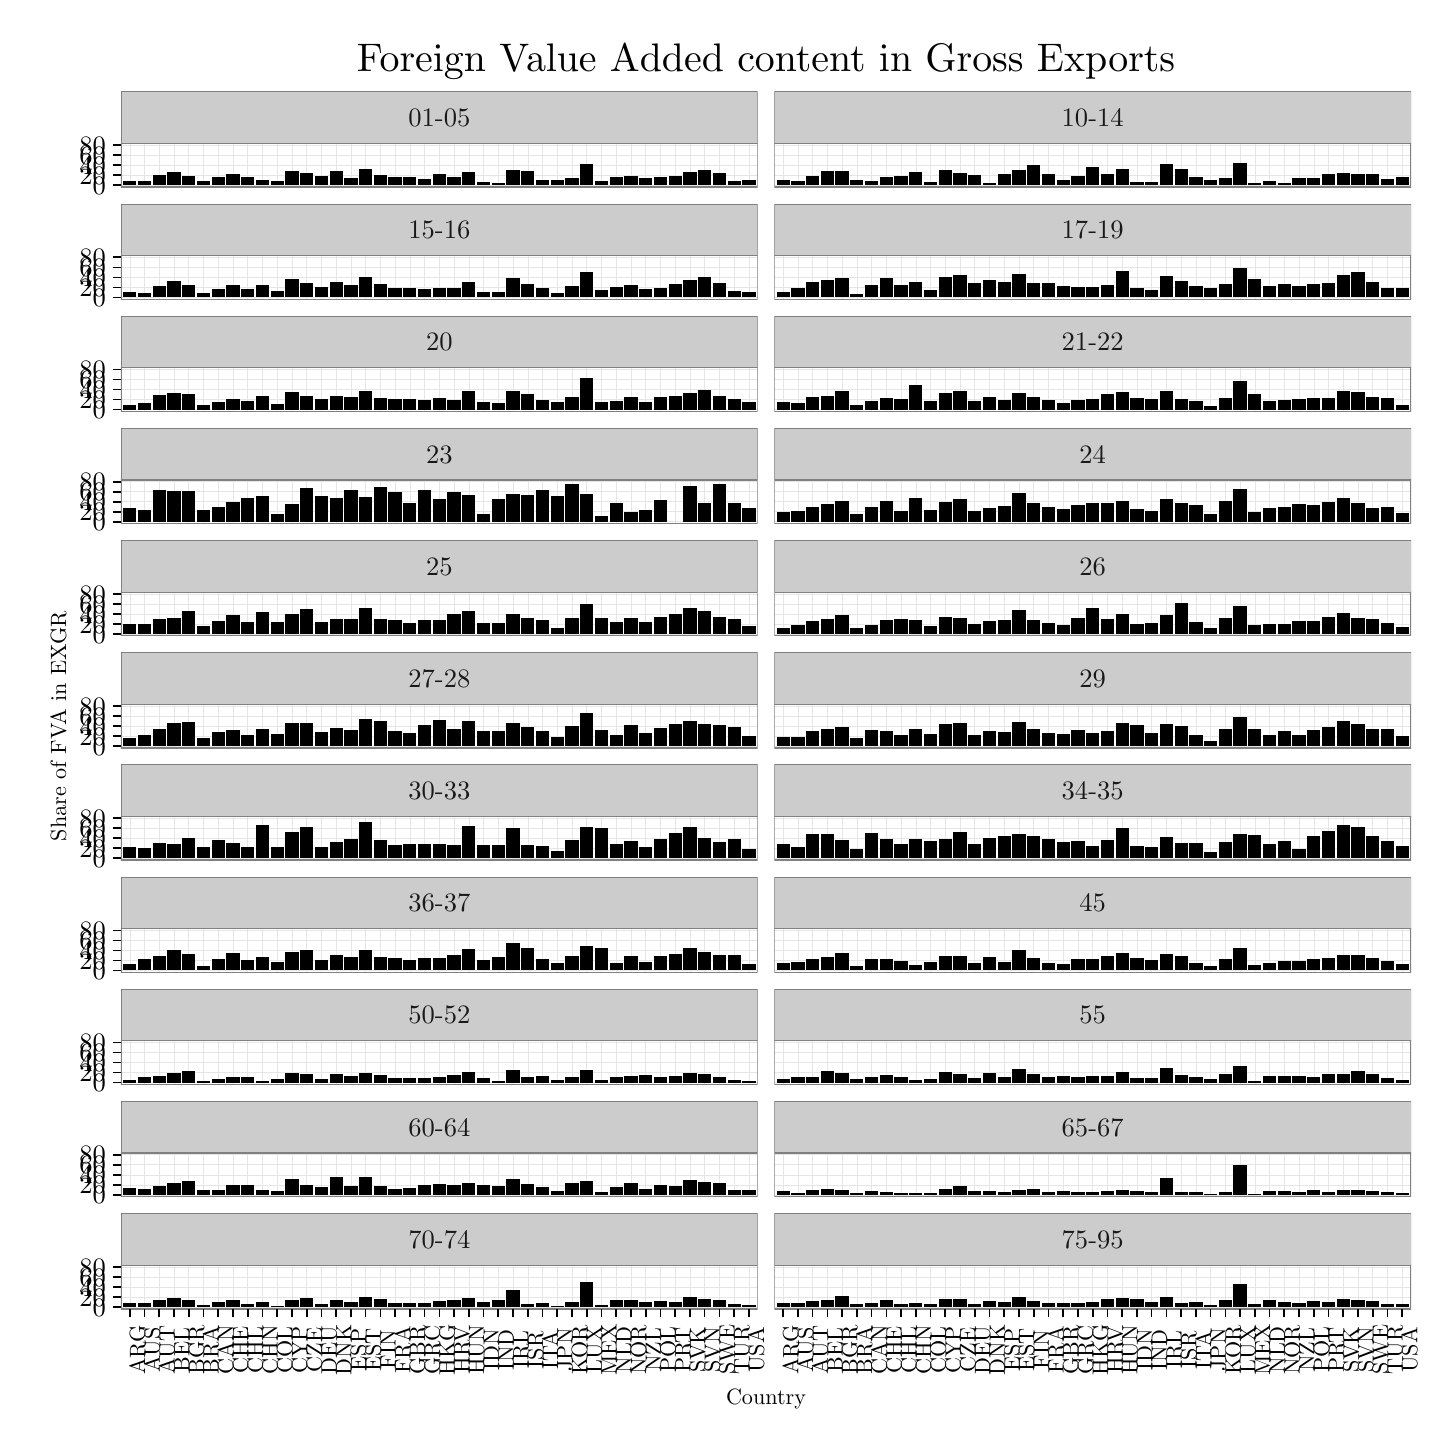
\begin{tikzpicture}[x=1pt,y=1pt]
\definecolor{fillColor}{RGB}{255,255,255}
\path[use as bounding box,fill=fillColor,fill opacity=0.00] (0,0) rectangle (505.89,505.89);
\begin{scope}
\path[clip] (  0.00,  0.00) rectangle (505.89,505.89);
\definecolor{drawColor}{RGB}{255,255,255}
\definecolor{fillColor}{RGB}{255,255,255}

\path[draw=drawColor,line width= 0.6pt,line join=round,line cap=round,fill=fillColor] (  0.00,  0.00) rectangle (505.89,505.89);
\end{scope}
\begin{scope}
\path[clip] ( 33.71,448.24) rectangle (263.80,464.16);
\definecolor{fillColor}{RGB}{255,255,255}

\path[fill=fillColor] ( 33.71,448.24) rectangle (263.80,464.16);
\definecolor{drawColor}{gray}{0.90}

\path[draw=drawColor,line width= 0.2pt,line join=round] ( 33.71,448.96) --
	(263.80,448.96);

\path[draw=drawColor,line width= 0.2pt,line join=round] ( 33.71,452.58) --
	(263.80,452.58);

\path[draw=drawColor,line width= 0.2pt,line join=round] ( 33.71,456.20) --
	(263.80,456.20);

\path[draw=drawColor,line width= 0.2pt,line join=round] ( 33.71,459.82) --
	(263.80,459.82);

\path[draw=drawColor,line width= 0.2pt,line join=round] ( 33.71,463.44) --
	(263.80,463.44);

\path[draw=drawColor,line width= 0.2pt,line join=round] ( 36.90,448.24) --
	( 36.90,464.16);

\path[draw=drawColor,line width= 0.2pt,line join=round] ( 42.23,448.24) --
	( 42.23,464.16);

\path[draw=drawColor,line width= 0.2pt,line join=round] ( 47.56,448.24) --
	( 47.56,464.16);

\path[draw=drawColor,line width= 0.2pt,line join=round] ( 52.88,448.24) --
	( 52.88,464.16);

\path[draw=drawColor,line width= 0.2pt,line join=round] ( 58.21,448.24) --
	( 58.21,464.16);

\path[draw=drawColor,line width= 0.2pt,line join=round] ( 63.53,448.24) --
	( 63.53,464.16);

\path[draw=drawColor,line width= 0.2pt,line join=round] ( 68.86,448.24) --
	( 68.86,464.16);

\path[draw=drawColor,line width= 0.2pt,line join=round] ( 74.19,448.24) --
	( 74.19,464.16);

\path[draw=drawColor,line width= 0.2pt,line join=round] ( 79.51,448.24) --
	( 79.51,464.16);

\path[draw=drawColor,line width= 0.2pt,line join=round] ( 84.84,448.24) --
	( 84.84,464.16);

\path[draw=drawColor,line width= 0.2pt,line join=round] ( 90.17,448.24) --
	( 90.17,464.16);

\path[draw=drawColor,line width= 0.2pt,line join=round] ( 95.49,448.24) --
	( 95.49,464.16);

\path[draw=drawColor,line width= 0.2pt,line join=round] (100.82,448.24) --
	(100.82,464.16);

\path[draw=drawColor,line width= 0.2pt,line join=round] (106.14,448.24) --
	(106.14,464.16);

\path[draw=drawColor,line width= 0.2pt,line join=round] (111.47,448.24) --
	(111.47,464.16);

\path[draw=drawColor,line width= 0.2pt,line join=round] (116.80,448.24) --
	(116.80,464.16);

\path[draw=drawColor,line width= 0.2pt,line join=round] (122.12,448.24) --
	(122.12,464.16);

\path[draw=drawColor,line width= 0.2pt,line join=round] (127.45,448.24) --
	(127.45,464.16);

\path[draw=drawColor,line width= 0.2pt,line join=round] (132.77,448.24) --
	(132.77,464.16);

\path[draw=drawColor,line width= 0.2pt,line join=round] (138.10,448.24) --
	(138.10,464.16);

\path[draw=drawColor,line width= 0.2pt,line join=round] (143.43,448.24) --
	(143.43,464.16);

\path[draw=drawColor,line width= 0.2pt,line join=round] (148.75,448.24) --
	(148.75,464.16);

\path[draw=drawColor,line width= 0.2pt,line join=round] (154.08,448.24) --
	(154.08,464.16);

\path[draw=drawColor,line width= 0.2pt,line join=round] (159.41,448.24) --
	(159.41,464.16);

\path[draw=drawColor,line width= 0.2pt,line join=round] (164.73,448.24) --
	(164.73,464.16);

\path[draw=drawColor,line width= 0.2pt,line join=round] (170.06,448.24) --
	(170.06,464.16);

\path[draw=drawColor,line width= 0.2pt,line join=round] (175.38,448.24) --
	(175.38,464.16);

\path[draw=drawColor,line width= 0.2pt,line join=round] (180.71,448.24) --
	(180.71,464.16);

\path[draw=drawColor,line width= 0.2pt,line join=round] (186.04,448.24) --
	(186.04,464.16);

\path[draw=drawColor,line width= 0.2pt,line join=round] (191.36,448.24) --
	(191.36,464.16);

\path[draw=drawColor,line width= 0.2pt,line join=round] (196.69,448.24) --
	(196.69,464.16);

\path[draw=drawColor,line width= 0.2pt,line join=round] (202.01,448.24) --
	(202.01,464.16);

\path[draw=drawColor,line width= 0.2pt,line join=round] (207.34,448.24) --
	(207.34,464.16);

\path[draw=drawColor,line width= 0.2pt,line join=round] (212.67,448.24) --
	(212.67,464.16);

\path[draw=drawColor,line width= 0.2pt,line join=round] (217.99,448.24) --
	(217.99,464.16);

\path[draw=drawColor,line width= 0.2pt,line join=round] (223.32,448.24) --
	(223.32,464.16);

\path[draw=drawColor,line width= 0.2pt,line join=round] (228.65,448.24) --
	(228.65,464.16);

\path[draw=drawColor,line width= 0.2pt,line join=round] (233.97,448.24) --
	(233.97,464.16);

\path[draw=drawColor,line width= 0.2pt,line join=round] (239.30,448.24) --
	(239.30,464.16);

\path[draw=drawColor,line width= 0.2pt,line join=round] (244.62,448.24) --
	(244.62,464.16);

\path[draw=drawColor,line width= 0.2pt,line join=round] (249.95,448.24) --
	(249.95,464.16);

\path[draw=drawColor,line width= 0.2pt,line join=round] (255.28,448.24) --
	(255.28,464.16);

\path[draw=drawColor,line width= 0.2pt,line join=round] (260.60,448.24) --
	(260.60,464.16);
\definecolor{fillColor}{RGB}{0,0,0}

\path[fill=fillColor] ( 34.51,448.96) rectangle ( 39.30,450.38);

\path[fill=fillColor] ( 39.83,448.96) rectangle ( 44.63,450.47);

\path[fill=fillColor] ( 45.16,448.96) rectangle ( 49.95,452.55);

\path[fill=fillColor] ( 50.48,448.96) rectangle ( 55.28,453.60);

\path[fill=fillColor] ( 55.81,448.96) rectangle ( 60.60,452.15);

\path[fill=fillColor] ( 61.14,448.96) rectangle ( 65.93,450.57);

\path[fill=fillColor] ( 66.46,448.96) rectangle ( 71.26,451.90);

\path[fill=fillColor] ( 71.79,448.96) rectangle ( 76.58,452.91);

\path[fill=fillColor] ( 77.12,448.96) rectangle ( 81.91,451.76);

\path[fill=fillColor] ( 82.44,448.96) rectangle ( 87.24,450.78);

\path[fill=fillColor] ( 87.77,448.96) rectangle ( 92.56,450.37);

\path[fill=fillColor] ( 93.09,448.96) rectangle ( 97.89,454.02);

\path[fill=fillColor] ( 98.42,448.96) rectangle (103.21,453.31);

\path[fill=fillColor] (103.75,448.96) rectangle (108.54,452.14);

\path[fill=fillColor] (109.07,448.96) rectangle (113.87,453.96);

\path[fill=fillColor] (114.40,448.96) rectangle (119.19,451.67);

\path[fill=fillColor] (119.73,448.96) rectangle (124.52,454.81);

\path[fill=fillColor] (125.05,448.96) rectangle (129.85,452.51);

\path[fill=fillColor] (130.38,448.96) rectangle (135.17,452.05);

\path[fill=fillColor] (135.70,448.96) rectangle (140.50,452.04);

\path[fill=fillColor] (141.03,448.96) rectangle (145.82,451.14);

\path[fill=fillColor] (146.36,448.96) rectangle (151.15,452.93);

\path[fill=fillColor] (151.68,448.96) rectangle (156.48,451.93);

\path[fill=fillColor] (157.01,448.96) rectangle (161.80,453.61);

\path[fill=fillColor] (162.33,448.96) rectangle (167.13,450.16);

\path[fill=fillColor] (167.66,448.96) rectangle (172.45,449.69);

\path[fill=fillColor] (172.99,448.96) rectangle (177.78,454.52);

\path[fill=fillColor] (178.31,448.96) rectangle (183.11,454.24);

\path[fill=fillColor] (183.64,448.96) rectangle (188.43,451.01);

\path[fill=fillColor] (188.97,448.96) rectangle (193.76,450.68);

\path[fill=fillColor] (194.29,448.96) rectangle (199.09,451.47);

\path[fill=fillColor] (199.62,448.96) rectangle (204.41,456.73);

\path[fill=fillColor] (204.94,448.96) rectangle (209.74,450.56);

\path[fill=fillColor] (210.27,448.96) rectangle (215.06,451.83);

\path[fill=fillColor] (215.60,448.96) rectangle (220.39,452.29);

\path[fill=fillColor] (220.92,448.96) rectangle (225.72,451.46);

\path[fill=fillColor] (226.25,448.96) rectangle (231.04,451.89);

\path[fill=fillColor] (231.58,448.96) rectangle (236.37,452.20);

\path[fill=fillColor] (236.90,448.96) rectangle (241.70,453.71);

\path[fill=fillColor] (242.23,448.96) rectangle (247.02,454.56);

\path[fill=fillColor] (247.55,448.96) rectangle (252.35,453.30);

\path[fill=fillColor] (252.88,448.96) rectangle (257.67,450.35);

\path[fill=fillColor] (258.21,448.96) rectangle (263.00,450.80);
\definecolor{drawColor}{gray}{0.50}

\path[draw=drawColor,line width= 0.6pt,line join=round,line cap=round] ( 33.71,448.24) rectangle (263.80,464.16);
\end{scope}
\begin{scope}
\path[clip] (269.80,448.24) rectangle (499.89,464.16);
\definecolor{fillColor}{RGB}{255,255,255}

\path[fill=fillColor] (269.80,448.24) rectangle (499.89,464.16);
\definecolor{drawColor}{gray}{0.90}

\path[draw=drawColor,line width= 0.2pt,line join=round] (269.80,448.96) --
	(499.89,448.96);

\path[draw=drawColor,line width= 0.2pt,line join=round] (269.80,452.58) --
	(499.89,452.58);

\path[draw=drawColor,line width= 0.2pt,line join=round] (269.80,456.20) --
	(499.89,456.20);

\path[draw=drawColor,line width= 0.2pt,line join=round] (269.80,459.82) --
	(499.89,459.82);

\path[draw=drawColor,line width= 0.2pt,line join=round] (269.80,463.44) --
	(499.89,463.44);

\path[draw=drawColor,line width= 0.2pt,line join=round] (272.99,448.24) --
	(272.99,464.16);

\path[draw=drawColor,line width= 0.2pt,line join=round] (278.32,448.24) --
	(278.32,464.16);

\path[draw=drawColor,line width= 0.2pt,line join=round] (283.65,448.24) --
	(283.65,464.16);

\path[draw=drawColor,line width= 0.2pt,line join=round] (288.97,448.24) --
	(288.97,464.16);

\path[draw=drawColor,line width= 0.2pt,line join=round] (294.30,448.24) --
	(294.30,464.16);

\path[draw=drawColor,line width= 0.2pt,line join=round] (299.63,448.24) --
	(299.63,464.16);

\path[draw=drawColor,line width= 0.2pt,line join=round] (304.95,448.24) --
	(304.95,464.16);

\path[draw=drawColor,line width= 0.2pt,line join=round] (310.28,448.24) --
	(310.28,464.16);

\path[draw=drawColor,line width= 0.2pt,line join=round] (315.60,448.24) --
	(315.60,464.16);

\path[draw=drawColor,line width= 0.2pt,line join=round] (320.93,448.24) --
	(320.93,464.16);

\path[draw=drawColor,line width= 0.2pt,line join=round] (326.26,448.24) --
	(326.26,464.16);

\path[draw=drawColor,line width= 0.2pt,line join=round] (331.58,448.24) --
	(331.58,464.16);

\path[draw=drawColor,line width= 0.2pt,line join=round] (336.91,448.24) --
	(336.91,464.16);

\path[draw=drawColor,line width= 0.2pt,line join=round] (342.23,448.24) --
	(342.23,464.16);

\path[draw=drawColor,line width= 0.2pt,line join=round] (347.56,448.24) --
	(347.56,464.16);

\path[draw=drawColor,line width= 0.2pt,line join=round] (352.89,448.24) --
	(352.89,464.16);

\path[draw=drawColor,line width= 0.2pt,line join=round] (358.21,448.24) --
	(358.21,464.16);

\path[draw=drawColor,line width= 0.2pt,line join=round] (363.54,448.24) --
	(363.54,464.16);

\path[draw=drawColor,line width= 0.2pt,line join=round] (368.87,448.24) --
	(368.87,464.16);

\path[draw=drawColor,line width= 0.2pt,line join=round] (374.19,448.24) --
	(374.19,464.16);

\path[draw=drawColor,line width= 0.2pt,line join=round] (379.52,448.24) --
	(379.52,464.16);

\path[draw=drawColor,line width= 0.2pt,line join=round] (384.84,448.24) --
	(384.84,464.16);

\path[draw=drawColor,line width= 0.2pt,line join=round] (390.17,448.24) --
	(390.17,464.16);

\path[draw=drawColor,line width= 0.2pt,line join=round] (395.50,448.24) --
	(395.50,464.16);

\path[draw=drawColor,line width= 0.2pt,line join=round] (400.82,448.24) --
	(400.82,464.16);

\path[draw=drawColor,line width= 0.2pt,line join=round] (406.15,448.24) --
	(406.15,464.16);

\path[draw=drawColor,line width= 0.2pt,line join=round] (411.48,448.24) --
	(411.48,464.16);

\path[draw=drawColor,line width= 0.2pt,line join=round] (416.80,448.24) --
	(416.80,464.16);

\path[draw=drawColor,line width= 0.2pt,line join=round] (422.13,448.24) --
	(422.13,464.16);

\path[draw=drawColor,line width= 0.2pt,line join=round] (427.45,448.24) --
	(427.45,464.16);

\path[draw=drawColor,line width= 0.2pt,line join=round] (432.78,448.24) --
	(432.78,464.16);

\path[draw=drawColor,line width= 0.2pt,line join=round] (438.11,448.24) --
	(438.11,464.16);

\path[draw=drawColor,line width= 0.2pt,line join=round] (443.43,448.24) --
	(443.43,464.16);

\path[draw=drawColor,line width= 0.2pt,line join=round] (448.76,448.24) --
	(448.76,464.16);

\path[draw=drawColor,line width= 0.2pt,line join=round] (454.08,448.24) --
	(454.08,464.16);

\path[draw=drawColor,line width= 0.2pt,line join=round] (459.41,448.24) --
	(459.41,464.16);

\path[draw=drawColor,line width= 0.2pt,line join=round] (464.74,448.24) --
	(464.74,464.16);

\path[draw=drawColor,line width= 0.2pt,line join=round] (470.06,448.24) --
	(470.06,464.16);

\path[draw=drawColor,line width= 0.2pt,line join=round] (475.39,448.24) --
	(475.39,464.16);

\path[draw=drawColor,line width= 0.2pt,line join=round] (480.72,448.24) --
	(480.72,464.16);

\path[draw=drawColor,line width= 0.2pt,line join=round] (486.04,448.24) --
	(486.04,464.16);

\path[draw=drawColor,line width= 0.2pt,line join=round] (491.37,448.24) --
	(491.37,464.16);

\path[draw=drawColor,line width= 0.2pt,line join=round] (496.69,448.24) --
	(496.69,464.16);
\definecolor{fillColor}{RGB}{0,0,0}

\path[fill=fillColor] (270.60,448.96) rectangle (275.39,450.82);

\path[fill=fillColor] (275.92,448.96) rectangle (280.72,450.51);

\path[fill=fillColor] (281.25,448.96) rectangle (286.04,452.21);

\path[fill=fillColor] (286.58,448.96) rectangle (291.37,454.01);

\path[fill=fillColor] (291.90,448.96) rectangle (296.70,454.22);

\path[fill=fillColor] (297.23,448.96) rectangle (302.02,450.88);

\path[fill=fillColor] (302.55,448.96) rectangle (307.35,450.47);

\path[fill=fillColor] (307.88,448.96) rectangle (312.67,451.99);

\path[fill=fillColor] (313.21,448.96) rectangle (318.00,452.21);

\path[fill=fillColor] (318.53,448.96) rectangle (323.33,453.77);

\path[fill=fillColor] (323.86,448.96) rectangle (328.65,450.08);

\path[fill=fillColor] (329.19,448.96) rectangle (333.98,454.60);

\path[fill=fillColor] (334.51,448.96) rectangle (339.31,453.41);

\path[fill=fillColor] (339.84,448.96) rectangle (344.63,452.73);

\path[fill=fillColor] (345.16,448.96) rectangle (349.96,449.62);

\path[fill=fillColor] (350.49,448.96) rectangle (355.28,453.07);

\path[fill=fillColor] (355.82,448.96) rectangle (360.61,454.57);

\path[fill=fillColor] (361.14,448.96) rectangle (365.94,456.29);

\path[fill=fillColor] (366.47,448.96) rectangle (371.26,453.18);

\path[fill=fillColor] (371.80,448.96) rectangle (376.59,450.68);

\path[fill=fillColor] (377.12,448.96) rectangle (381.91,452.26);

\path[fill=fillColor] (382.45,448.96) rectangle (387.24,455.43);

\path[fill=fillColor] (387.77,448.96) rectangle (392.57,453.16);

\path[fill=fillColor] (393.10,448.96) rectangle (397.89,454.92);

\path[fill=fillColor] (398.43,448.96) rectangle (403.22,450.19);

\path[fill=fillColor] (403.75,448.96) rectangle (408.55,450.10);

\path[fill=fillColor] (409.08,448.96) rectangle (413.87,456.71);

\path[fill=fillColor] (414.40,448.96) rectangle (419.20,454.78);

\path[fill=fillColor] (419.73,448.96) rectangle (424.52,451.85);

\path[fill=fillColor] (425.06,448.96) rectangle (429.85,450.70);

\path[fill=fillColor] (430.38,448.96) rectangle (435.18,451.65);

\path[fill=fillColor] (435.71,448.96) rectangle (440.50,457.08);

\path[fill=fillColor] (441.04,448.96) rectangle (445.83,449.72);

\path[fill=fillColor] (446.36,448.96) rectangle (451.16,450.55);

\path[fill=fillColor] (451.69,448.96) rectangle (456.48,449.87);

\path[fill=fillColor] (457.01,448.96) rectangle (461.81,451.64);

\path[fill=fillColor] (462.34,448.96) rectangle (467.13,451.54);

\path[fill=fillColor] (467.67,448.96) rectangle (472.46,453.15);

\path[fill=fillColor] (472.99,448.96) rectangle (477.79,453.27);

\path[fill=fillColor] (478.32,448.96) rectangle (483.11,452.93);

\path[fill=fillColor] (483.65,448.96) rectangle (488.44,453.05);

\path[fill=fillColor] (488.97,448.96) rectangle (493.76,451.17);

\path[fill=fillColor] (494.30,448.96) rectangle (499.09,451.83);
\definecolor{drawColor}{gray}{0.50}

\path[draw=drawColor,line width= 0.6pt,line join=round,line cap=round] (269.80,448.24) rectangle (499.89,464.16);
\end{scope}
\begin{scope}
\path[clip] ( 33.71,407.70) rectangle (263.80,423.63);
\definecolor{fillColor}{RGB}{255,255,255}

\path[fill=fillColor] ( 33.71,407.70) rectangle (263.80,423.63);
\definecolor{drawColor}{gray}{0.90}

\path[draw=drawColor,line width= 0.2pt,line join=round] ( 33.71,408.43) --
	(263.80,408.43);

\path[draw=drawColor,line width= 0.2pt,line join=round] ( 33.71,412.04) --
	(263.80,412.04);

\path[draw=drawColor,line width= 0.2pt,line join=round] ( 33.71,415.66) --
	(263.80,415.66);

\path[draw=drawColor,line width= 0.2pt,line join=round] ( 33.71,419.28) --
	(263.80,419.28);

\path[draw=drawColor,line width= 0.2pt,line join=round] ( 33.71,422.90) --
	(263.80,422.90);

\path[draw=drawColor,line width= 0.2pt,line join=round] ( 36.90,407.70) --
	( 36.90,423.63);

\path[draw=drawColor,line width= 0.2pt,line join=round] ( 42.23,407.70) --
	( 42.23,423.63);

\path[draw=drawColor,line width= 0.2pt,line join=round] ( 47.56,407.70) --
	( 47.56,423.63);

\path[draw=drawColor,line width= 0.2pt,line join=round] ( 52.88,407.70) --
	( 52.88,423.63);

\path[draw=drawColor,line width= 0.2pt,line join=round] ( 58.21,407.70) --
	( 58.21,423.63);

\path[draw=drawColor,line width= 0.2pt,line join=round] ( 63.53,407.70) --
	( 63.53,423.63);

\path[draw=drawColor,line width= 0.2pt,line join=round] ( 68.86,407.70) --
	( 68.86,423.63);

\path[draw=drawColor,line width= 0.2pt,line join=round] ( 74.19,407.70) --
	( 74.19,423.63);

\path[draw=drawColor,line width= 0.2pt,line join=round] ( 79.51,407.70) --
	( 79.51,423.63);

\path[draw=drawColor,line width= 0.2pt,line join=round] ( 84.84,407.70) --
	( 84.84,423.63);

\path[draw=drawColor,line width= 0.2pt,line join=round] ( 90.17,407.70) --
	( 90.17,423.63);

\path[draw=drawColor,line width= 0.2pt,line join=round] ( 95.49,407.70) --
	( 95.49,423.63);

\path[draw=drawColor,line width= 0.2pt,line join=round] (100.82,407.70) --
	(100.82,423.63);

\path[draw=drawColor,line width= 0.2pt,line join=round] (106.14,407.70) --
	(106.14,423.63);

\path[draw=drawColor,line width= 0.2pt,line join=round] (111.47,407.70) --
	(111.47,423.63);

\path[draw=drawColor,line width= 0.2pt,line join=round] (116.80,407.70) --
	(116.80,423.63);

\path[draw=drawColor,line width= 0.2pt,line join=round] (122.12,407.70) --
	(122.12,423.63);

\path[draw=drawColor,line width= 0.2pt,line join=round] (127.45,407.70) --
	(127.45,423.63);

\path[draw=drawColor,line width= 0.2pt,line join=round] (132.77,407.70) --
	(132.77,423.63);

\path[draw=drawColor,line width= 0.2pt,line join=round] (138.10,407.70) --
	(138.10,423.63);

\path[draw=drawColor,line width= 0.2pt,line join=round] (143.43,407.70) --
	(143.43,423.63);

\path[draw=drawColor,line width= 0.2pt,line join=round] (148.75,407.70) --
	(148.75,423.63);

\path[draw=drawColor,line width= 0.2pt,line join=round] (154.08,407.70) --
	(154.08,423.63);

\path[draw=drawColor,line width= 0.2pt,line join=round] (159.41,407.70) --
	(159.41,423.63);

\path[draw=drawColor,line width= 0.2pt,line join=round] (164.73,407.70) --
	(164.73,423.63);

\path[draw=drawColor,line width= 0.2pt,line join=round] (170.06,407.70) --
	(170.06,423.63);

\path[draw=drawColor,line width= 0.2pt,line join=round] (175.38,407.70) --
	(175.38,423.63);

\path[draw=drawColor,line width= 0.2pt,line join=round] (180.71,407.70) --
	(180.71,423.63);

\path[draw=drawColor,line width= 0.2pt,line join=round] (186.04,407.70) --
	(186.04,423.63);

\path[draw=drawColor,line width= 0.2pt,line join=round] (191.36,407.70) --
	(191.36,423.63);

\path[draw=drawColor,line width= 0.2pt,line join=round] (196.69,407.70) --
	(196.69,423.63);

\path[draw=drawColor,line width= 0.2pt,line join=round] (202.01,407.70) --
	(202.01,423.63);

\path[draw=drawColor,line width= 0.2pt,line join=round] (207.34,407.70) --
	(207.34,423.63);

\path[draw=drawColor,line width= 0.2pt,line join=round] (212.67,407.70) --
	(212.67,423.63);

\path[draw=drawColor,line width= 0.2pt,line join=round] (217.99,407.70) --
	(217.99,423.63);

\path[draw=drawColor,line width= 0.2pt,line join=round] (223.32,407.70) --
	(223.32,423.63);

\path[draw=drawColor,line width= 0.2pt,line join=round] (228.65,407.70) --
	(228.65,423.63);

\path[draw=drawColor,line width= 0.2pt,line join=round] (233.97,407.70) --
	(233.97,423.63);

\path[draw=drawColor,line width= 0.2pt,line join=round] (239.30,407.70) --
	(239.30,423.63);

\path[draw=drawColor,line width= 0.2pt,line join=round] (244.62,407.70) --
	(244.62,423.63);

\path[draw=drawColor,line width= 0.2pt,line join=round] (249.95,407.70) --
	(249.95,423.63);

\path[draw=drawColor,line width= 0.2pt,line join=round] (255.28,407.70) --
	(255.28,423.63);

\path[draw=drawColor,line width= 0.2pt,line join=round] (260.60,407.70) --
	(260.60,423.63);
\definecolor{fillColor}{RGB}{0,0,0}

\path[fill=fillColor] ( 34.51,408.43) rectangle ( 39.30,410.28);

\path[fill=fillColor] ( 39.83,408.43) rectangle ( 44.63,410.09);

\path[fill=fillColor] ( 45.16,408.43) rectangle ( 49.95,412.66);

\path[fill=fillColor] ( 50.48,408.43) rectangle ( 55.28,414.28);

\path[fill=fillColor] ( 55.81,408.43) rectangle ( 60.60,412.86);

\path[fill=fillColor] ( 61.14,408.43) rectangle ( 65.93,410.05);

\path[fill=fillColor] ( 66.46,408.43) rectangle ( 71.26,411.53);

\path[fill=fillColor] ( 71.79,408.43) rectangle ( 76.58,412.76);

\path[fill=fillColor] ( 77.12,408.43) rectangle ( 81.91,411.38);

\path[fill=fillColor] ( 82.44,408.43) rectangle ( 87.24,412.99);

\path[fill=fillColor] ( 87.77,408.43) rectangle ( 92.56,410.62);

\path[fill=fillColor] ( 93.09,408.43) rectangle ( 97.89,414.92);

\path[fill=fillColor] ( 98.42,408.43) rectangle (103.21,413.52);

\path[fill=fillColor] (103.75,408.43) rectangle (108.54,412.10);

\path[fill=fillColor] (109.07,408.43) rectangle (113.87,413.82);

\path[fill=fillColor] (114.40,408.43) rectangle (119.19,412.82);

\path[fill=fillColor] (119.73,408.43) rectangle (124.52,415.83);

\path[fill=fillColor] (125.05,408.43) rectangle (129.85,413.18);

\path[fill=fillColor] (130.38,408.43) rectangle (135.17,411.78);

\path[fill=fillColor] (135.70,408.43) rectangle (140.50,411.86);

\path[fill=fillColor] (141.03,408.43) rectangle (145.82,411.45);

\path[fill=fillColor] (146.36,408.43) rectangle (151.15,411.99);

\path[fill=fillColor] (151.68,408.43) rectangle (156.48,411.87);

\path[fill=fillColor] (157.01,408.43) rectangle (161.80,414.09);

\path[fill=fillColor] (162.33,408.43) rectangle (167.13,410.34);

\path[fill=fillColor] (167.66,408.43) rectangle (172.45,410.49);

\path[fill=fillColor] (172.99,408.43) rectangle (177.78,415.40);

\path[fill=fillColor] (178.31,408.43) rectangle (183.11,413.43);

\path[fill=fillColor] (183.64,408.43) rectangle (188.43,411.93);

\path[fill=fillColor] (188.97,408.43) rectangle (193.76,410.16);

\path[fill=fillColor] (194.29,408.43) rectangle (199.09,412.42);

\path[fill=fillColor] (199.62,408.43) rectangle (204.41,417.66);

\path[fill=fillColor] (204.94,408.43) rectangle (209.74,411.08);

\path[fill=fillColor] (210.27,408.43) rectangle (215.06,412.13);

\path[fill=fillColor] (215.60,408.43) rectangle (220.39,412.87);

\path[fill=fillColor] (220.92,408.43) rectangle (225.72,411.49);

\path[fill=fillColor] (226.25,408.43) rectangle (231.04,411.93);

\path[fill=fillColor] (231.58,408.43) rectangle (236.37,413.21);

\path[fill=fillColor] (236.90,408.43) rectangle (241.70,414.57);

\path[fill=fillColor] (242.23,408.43) rectangle (247.02,415.72);

\path[fill=fillColor] (247.55,408.43) rectangle (252.35,413.50);

\path[fill=fillColor] (252.88,408.43) rectangle (257.67,410.78);

\path[fill=fillColor] (258.21,408.43) rectangle (263.00,410.50);
\definecolor{drawColor}{gray}{0.50}

\path[draw=drawColor,line width= 0.6pt,line join=round,line cap=round] ( 33.71,407.70) rectangle (263.80,423.63);
\end{scope}
\begin{scope}
\path[clip] (269.80,407.70) rectangle (499.89,423.63);
\definecolor{fillColor}{RGB}{255,255,255}

\path[fill=fillColor] (269.80,407.70) rectangle (499.89,423.63);
\definecolor{drawColor}{gray}{0.90}

\path[draw=drawColor,line width= 0.2pt,line join=round] (269.80,408.43) --
	(499.89,408.43);

\path[draw=drawColor,line width= 0.2pt,line join=round] (269.80,412.04) --
	(499.89,412.04);

\path[draw=drawColor,line width= 0.2pt,line join=round] (269.80,415.66) --
	(499.89,415.66);

\path[draw=drawColor,line width= 0.2pt,line join=round] (269.80,419.28) --
	(499.89,419.28);

\path[draw=drawColor,line width= 0.2pt,line join=round] (269.80,422.90) --
	(499.89,422.90);

\path[draw=drawColor,line width= 0.2pt,line join=round] (272.99,407.70) --
	(272.99,423.63);

\path[draw=drawColor,line width= 0.2pt,line join=round] (278.32,407.70) --
	(278.32,423.63);

\path[draw=drawColor,line width= 0.2pt,line join=round] (283.65,407.70) --
	(283.65,423.63);

\path[draw=drawColor,line width= 0.2pt,line join=round] (288.97,407.70) --
	(288.97,423.63);

\path[draw=drawColor,line width= 0.2pt,line join=round] (294.30,407.70) --
	(294.30,423.63);

\path[draw=drawColor,line width= 0.2pt,line join=round] (299.63,407.70) --
	(299.63,423.63);

\path[draw=drawColor,line width= 0.2pt,line join=round] (304.95,407.70) --
	(304.95,423.63);

\path[draw=drawColor,line width= 0.2pt,line join=round] (310.28,407.70) --
	(310.28,423.63);

\path[draw=drawColor,line width= 0.2pt,line join=round] (315.60,407.70) --
	(315.60,423.63);

\path[draw=drawColor,line width= 0.2pt,line join=round] (320.93,407.70) --
	(320.93,423.63);

\path[draw=drawColor,line width= 0.2pt,line join=round] (326.26,407.70) --
	(326.26,423.63);

\path[draw=drawColor,line width= 0.2pt,line join=round] (331.58,407.70) --
	(331.58,423.63);

\path[draw=drawColor,line width= 0.2pt,line join=round] (336.91,407.70) --
	(336.91,423.63);

\path[draw=drawColor,line width= 0.2pt,line join=round] (342.23,407.70) --
	(342.23,423.63);

\path[draw=drawColor,line width= 0.2pt,line join=round] (347.56,407.70) --
	(347.56,423.63);

\path[draw=drawColor,line width= 0.2pt,line join=round] (352.89,407.70) --
	(352.89,423.63);

\path[draw=drawColor,line width= 0.2pt,line join=round] (358.21,407.70) --
	(358.21,423.63);

\path[draw=drawColor,line width= 0.2pt,line join=round] (363.54,407.70) --
	(363.54,423.63);

\path[draw=drawColor,line width= 0.2pt,line join=round] (368.87,407.70) --
	(368.87,423.63);

\path[draw=drawColor,line width= 0.2pt,line join=round] (374.19,407.70) --
	(374.19,423.63);

\path[draw=drawColor,line width= 0.2pt,line join=round] (379.52,407.70) --
	(379.52,423.63);

\path[draw=drawColor,line width= 0.2pt,line join=round] (384.84,407.70) --
	(384.84,423.63);

\path[draw=drawColor,line width= 0.2pt,line join=round] (390.17,407.70) --
	(390.17,423.63);

\path[draw=drawColor,line width= 0.2pt,line join=round] (395.50,407.70) --
	(395.50,423.63);

\path[draw=drawColor,line width= 0.2pt,line join=round] (400.82,407.70) --
	(400.82,423.63);

\path[draw=drawColor,line width= 0.2pt,line join=round] (406.15,407.70) --
	(406.15,423.63);

\path[draw=drawColor,line width= 0.2pt,line join=round] (411.48,407.70) --
	(411.48,423.63);

\path[draw=drawColor,line width= 0.2pt,line join=round] (416.80,407.70) --
	(416.80,423.63);

\path[draw=drawColor,line width= 0.2pt,line join=round] (422.13,407.70) --
	(422.13,423.63);

\path[draw=drawColor,line width= 0.2pt,line join=round] (427.45,407.70) --
	(427.45,423.63);

\path[draw=drawColor,line width= 0.2pt,line join=round] (432.78,407.70) --
	(432.78,423.63);

\path[draw=drawColor,line width= 0.2pt,line join=round] (438.11,407.70) --
	(438.11,423.63);

\path[draw=drawColor,line width= 0.2pt,line join=round] (443.43,407.70) --
	(443.43,423.63);

\path[draw=drawColor,line width= 0.2pt,line join=round] (448.76,407.70) --
	(448.76,423.63);

\path[draw=drawColor,line width= 0.2pt,line join=round] (454.08,407.70) --
	(454.08,423.63);

\path[draw=drawColor,line width= 0.2pt,line join=round] (459.41,407.70) --
	(459.41,423.63);

\path[draw=drawColor,line width= 0.2pt,line join=round] (464.74,407.70) --
	(464.74,423.63);

\path[draw=drawColor,line width= 0.2pt,line join=round] (470.06,407.70) --
	(470.06,423.63);

\path[draw=drawColor,line width= 0.2pt,line join=round] (475.39,407.70) --
	(475.39,423.63);

\path[draw=drawColor,line width= 0.2pt,line join=round] (480.72,407.70) --
	(480.72,423.63);

\path[draw=drawColor,line width= 0.2pt,line join=round] (486.04,407.70) --
	(486.04,423.63);

\path[draw=drawColor,line width= 0.2pt,line join=round] (491.37,407.70) --
	(491.37,423.63);

\path[draw=drawColor,line width= 0.2pt,line join=round] (496.69,407.70) --
	(496.69,423.63);
\definecolor{fillColor}{RGB}{0,0,0}

\path[fill=fillColor] (270.60,408.43) rectangle (275.39,410.37);

\path[fill=fillColor] (275.92,408.43) rectangle (280.72,411.76);

\path[fill=fillColor] (281.25,408.43) rectangle (286.04,414.02);

\path[fill=fillColor] (286.58,408.43) rectangle (291.37,414.61);

\path[fill=fillColor] (291.90,408.43) rectangle (296.70,415.29);

\path[fill=fillColor] (297.23,408.43) rectangle (302.02,409.81);

\path[fill=fillColor] (302.55,408.43) rectangle (307.35,413.07);

\path[fill=fillColor] (307.88,408.43) rectangle (312.67,415.58);

\path[fill=fillColor] (313.21,408.43) rectangle (318.00,412.73);

\path[fill=fillColor] (318.53,408.43) rectangle (323.33,414.02);

\path[fill=fillColor] (323.86,408.43) rectangle (328.65,411.17);

\path[fill=fillColor] (329.19,408.43) rectangle (333.98,415.71);

\path[fill=fillColor] (334.51,408.43) rectangle (339.31,416.55);

\path[fill=fillColor] (339.84,408.43) rectangle (344.63,413.51);

\path[fill=fillColor] (345.16,408.43) rectangle (349.96,414.84);

\path[fill=fillColor] (350.49,408.43) rectangle (355.28,414.05);

\path[fill=fillColor] (355.82,408.43) rectangle (360.61,416.94);

\path[fill=fillColor] (361.14,408.43) rectangle (365.94,413.70);

\path[fill=fillColor] (366.47,408.43) rectangle (371.26,413.50);

\path[fill=fillColor] (371.80,408.43) rectangle (376.59,412.46);

\path[fill=fillColor] (377.12,408.43) rectangle (381.91,412.25);

\path[fill=fillColor] (382.45,408.43) rectangle (387.24,412.12);

\path[fill=fillColor] (387.77,408.43) rectangle (392.57,412.76);

\path[fill=fillColor] (393.10,408.43) rectangle (397.89,417.87);

\path[fill=fillColor] (398.43,408.43) rectangle (403.22,411.92);

\path[fill=fillColor] (403.75,408.43) rectangle (408.55,411.13);

\path[fill=fillColor] (409.08,408.43) rectangle (413.87,416.05);

\path[fill=fillColor] (414.40,408.43) rectangle (419.20,414.22);

\path[fill=fillColor] (419.73,408.43) rectangle (424.52,412.58);

\path[fill=fillColor] (425.06,408.43) rectangle (429.85,411.97);

\path[fill=fillColor] (430.38,408.43) rectangle (435.18,413.32);

\path[fill=fillColor] (435.71,408.43) rectangle (440.50,419.06);

\path[fill=fillColor] (441.04,408.43) rectangle (445.83,415.14);

\path[fill=fillColor] (446.36,408.43) rectangle (451.16,412.67);

\path[fill=fillColor] (451.69,408.43) rectangle (456.48,413.27);

\path[fill=fillColor] (457.01,408.43) rectangle (461.81,412.64);

\path[fill=fillColor] (462.34,408.43) rectangle (467.13,413.43);

\path[fill=fillColor] (467.67,408.43) rectangle (472.46,413.71);

\path[fill=fillColor] (472.99,408.43) rectangle (477.79,416.39);

\path[fill=fillColor] (478.32,408.43) rectangle (483.11,417.72);

\path[fill=fillColor] (483.65,408.43) rectangle (488.44,413.84);

\path[fill=fillColor] (488.97,408.43) rectangle (493.76,411.96);

\path[fill=fillColor] (494.30,408.43) rectangle (499.09,411.95);
\definecolor{drawColor}{gray}{0.50}

\path[draw=drawColor,line width= 0.6pt,line join=round,line cap=round] (269.80,407.70) rectangle (499.89,423.63);
\end{scope}
\begin{scope}
\path[clip] ( 33.71,367.17) rectangle (263.80,383.09);
\definecolor{fillColor}{RGB}{255,255,255}

\path[fill=fillColor] ( 33.71,367.17) rectangle (263.80,383.09);
\definecolor{drawColor}{gray}{0.90}

\path[draw=drawColor,line width= 0.2pt,line join=round] ( 33.71,367.89) --
	(263.80,367.89);

\path[draw=drawColor,line width= 0.2pt,line join=round] ( 33.71,371.51) --
	(263.80,371.51);

\path[draw=drawColor,line width= 0.2pt,line join=round] ( 33.71,375.13) --
	(263.80,375.13);

\path[draw=drawColor,line width= 0.2pt,line join=round] ( 33.71,378.75) --
	(263.80,378.75);

\path[draw=drawColor,line width= 0.2pt,line join=round] ( 33.71,382.37) --
	(263.80,382.37);

\path[draw=drawColor,line width= 0.2pt,line join=round] ( 36.90,367.17) --
	( 36.90,383.09);

\path[draw=drawColor,line width= 0.2pt,line join=round] ( 42.23,367.17) --
	( 42.23,383.09);

\path[draw=drawColor,line width= 0.2pt,line join=round] ( 47.56,367.17) --
	( 47.56,383.09);

\path[draw=drawColor,line width= 0.2pt,line join=round] ( 52.88,367.17) --
	( 52.88,383.09);

\path[draw=drawColor,line width= 0.2pt,line join=round] ( 58.21,367.17) --
	( 58.21,383.09);

\path[draw=drawColor,line width= 0.2pt,line join=round] ( 63.53,367.17) --
	( 63.53,383.09);

\path[draw=drawColor,line width= 0.2pt,line join=round] ( 68.86,367.17) --
	( 68.86,383.09);

\path[draw=drawColor,line width= 0.2pt,line join=round] ( 74.19,367.17) --
	( 74.19,383.09);

\path[draw=drawColor,line width= 0.2pt,line join=round] ( 79.51,367.17) --
	( 79.51,383.09);

\path[draw=drawColor,line width= 0.2pt,line join=round] ( 84.84,367.17) --
	( 84.84,383.09);

\path[draw=drawColor,line width= 0.2pt,line join=round] ( 90.17,367.17) --
	( 90.17,383.09);

\path[draw=drawColor,line width= 0.2pt,line join=round] ( 95.49,367.17) --
	( 95.49,383.09);

\path[draw=drawColor,line width= 0.2pt,line join=round] (100.82,367.17) --
	(100.82,383.09);

\path[draw=drawColor,line width= 0.2pt,line join=round] (106.14,367.17) --
	(106.14,383.09);

\path[draw=drawColor,line width= 0.2pt,line join=round] (111.47,367.17) --
	(111.47,383.09);

\path[draw=drawColor,line width= 0.2pt,line join=round] (116.80,367.17) --
	(116.80,383.09);

\path[draw=drawColor,line width= 0.2pt,line join=round] (122.12,367.17) --
	(122.12,383.09);

\path[draw=drawColor,line width= 0.2pt,line join=round] (127.45,367.17) --
	(127.45,383.09);

\path[draw=drawColor,line width= 0.2pt,line join=round] (132.77,367.17) --
	(132.77,383.09);

\path[draw=drawColor,line width= 0.2pt,line join=round] (138.10,367.17) --
	(138.10,383.09);

\path[draw=drawColor,line width= 0.2pt,line join=round] (143.43,367.17) --
	(143.43,383.09);

\path[draw=drawColor,line width= 0.2pt,line join=round] (148.75,367.17) --
	(148.75,383.09);

\path[draw=drawColor,line width= 0.2pt,line join=round] (154.08,367.17) --
	(154.08,383.09);

\path[draw=drawColor,line width= 0.2pt,line join=round] (159.41,367.17) --
	(159.41,383.09);

\path[draw=drawColor,line width= 0.2pt,line join=round] (164.73,367.17) --
	(164.73,383.09);

\path[draw=drawColor,line width= 0.2pt,line join=round] (170.06,367.17) --
	(170.06,383.09);

\path[draw=drawColor,line width= 0.2pt,line join=round] (175.38,367.17) --
	(175.38,383.09);

\path[draw=drawColor,line width= 0.2pt,line join=round] (180.71,367.17) --
	(180.71,383.09);

\path[draw=drawColor,line width= 0.2pt,line join=round] (186.04,367.17) --
	(186.04,383.09);

\path[draw=drawColor,line width= 0.2pt,line join=round] (191.36,367.17) --
	(191.36,383.09);

\path[draw=drawColor,line width= 0.2pt,line join=round] (196.69,367.17) --
	(196.69,383.09);

\path[draw=drawColor,line width= 0.2pt,line join=round] (202.01,367.17) --
	(202.01,383.09);

\path[draw=drawColor,line width= 0.2pt,line join=round] (207.34,367.17) --
	(207.34,383.09);

\path[draw=drawColor,line width= 0.2pt,line join=round] (212.67,367.17) --
	(212.67,383.09);

\path[draw=drawColor,line width= 0.2pt,line join=round] (217.99,367.17) --
	(217.99,383.09);

\path[draw=drawColor,line width= 0.2pt,line join=round] (223.32,367.17) --
	(223.32,383.09);

\path[draw=drawColor,line width= 0.2pt,line join=round] (228.65,367.17) --
	(228.65,383.09);

\path[draw=drawColor,line width= 0.2pt,line join=round] (233.97,367.17) --
	(233.97,383.09);

\path[draw=drawColor,line width= 0.2pt,line join=round] (239.30,367.17) --
	(239.30,383.09);

\path[draw=drawColor,line width= 0.2pt,line join=round] (244.62,367.17) --
	(244.62,383.09);

\path[draw=drawColor,line width= 0.2pt,line join=round] (249.95,367.17) --
	(249.95,383.09);

\path[draw=drawColor,line width= 0.2pt,line join=round] (255.28,367.17) --
	(255.28,383.09);

\path[draw=drawColor,line width= 0.2pt,line join=round] (260.60,367.17) --
	(260.60,383.09);
\definecolor{fillColor}{RGB}{0,0,0}

\path[fill=fillColor] ( 34.51,367.89) rectangle ( 39.30,369.44);

\path[fill=fillColor] ( 39.83,367.89) rectangle ( 44.63,370.12);

\path[fill=fillColor] ( 45.16,367.89) rectangle ( 49.95,373.05);

\path[fill=fillColor] ( 50.48,367.89) rectangle ( 55.28,373.74);

\path[fill=fillColor] ( 55.81,367.89) rectangle ( 60.60,373.48);

\path[fill=fillColor] ( 61.14,367.89) rectangle ( 65.93,369.64);

\path[fill=fillColor] ( 66.46,367.89) rectangle ( 71.26,370.63);

\path[fill=fillColor] ( 71.79,367.89) rectangle ( 76.58,371.69);

\path[fill=fillColor] ( 77.12,367.89) rectangle ( 81.91,370.91);

\path[fill=fillColor] ( 82.44,367.89) rectangle ( 87.24,372.95);

\path[fill=fillColor] ( 87.77,367.89) rectangle ( 92.56,369.93);

\path[fill=fillColor] ( 93.09,367.89) rectangle ( 97.89,374.15);

\path[fill=fillColor] ( 98.42,367.89) rectangle (103.21,372.88);

\path[fill=fillColor] (103.75,367.89) rectangle (108.54,371.75);

\path[fill=fillColor] (109.07,367.89) rectangle (113.87,372.88);

\path[fill=fillColor] (114.40,367.89) rectangle (119.19,372.37);

\path[fill=fillColor] (119.73,367.89) rectangle (124.52,374.73);

\path[fill=fillColor] (125.05,367.89) rectangle (129.85,372.18);

\path[fill=fillColor] (130.38,367.89) rectangle (135.17,371.53);

\path[fill=fillColor] (135.70,367.89) rectangle (140.50,371.64);

\path[fill=fillColor] (141.03,367.89) rectangle (145.82,371.51);

\path[fill=fillColor] (146.36,367.89) rectangle (151.15,372.16);

\path[fill=fillColor] (151.68,367.89) rectangle (156.48,371.33);

\path[fill=fillColor] (157.01,367.89) rectangle (161.80,374.67);

\path[fill=fillColor] (162.33,367.89) rectangle (167.13,370.54);

\path[fill=fillColor] (167.66,367.89) rectangle (172.45,370.39);

\path[fill=fillColor] (172.99,367.89) rectangle (177.78,374.48);

\path[fill=fillColor] (178.31,367.89) rectangle (183.11,373.59);

\path[fill=fillColor] (183.64,367.89) rectangle (188.43,371.41);

\path[fill=fillColor] (188.97,367.89) rectangle (193.76,370.45);

\path[fill=fillColor] (194.29,367.89) rectangle (199.09,372.44);

\path[fill=fillColor] (199.62,367.89) rectangle (204.41,379.39);

\path[fill=fillColor] (204.94,367.89) rectangle (209.74,370.69);

\path[fill=fillColor] (210.27,367.89) rectangle (215.06,371.16);

\path[fill=fillColor] (215.60,367.89) rectangle (220.39,372.44);

\path[fill=fillColor] (220.92,367.89) rectangle (225.72,370.73);

\path[fill=fillColor] (226.25,367.89) rectangle (231.04,372.27);

\path[fill=fillColor] (231.58,367.89) rectangle (236.37,372.79);

\path[fill=fillColor] (236.90,367.89) rectangle (241.70,373.75);

\path[fill=fillColor] (242.23,367.89) rectangle (247.02,375.07);

\path[fill=fillColor] (247.55,367.89) rectangle (252.35,372.65);

\path[fill=fillColor] (252.88,367.89) rectangle (257.67,371.66);

\path[fill=fillColor] (258.21,367.89) rectangle (263.00,370.57);
\definecolor{drawColor}{gray}{0.50}

\path[draw=drawColor,line width= 0.6pt,line join=round,line cap=round] ( 33.71,367.17) rectangle (263.80,383.09);
\end{scope}
\begin{scope}
\path[clip] (269.80,367.17) rectangle (499.89,383.09);
\definecolor{fillColor}{RGB}{255,255,255}

\path[fill=fillColor] (269.80,367.17) rectangle (499.89,383.09);
\definecolor{drawColor}{gray}{0.90}

\path[draw=drawColor,line width= 0.2pt,line join=round] (269.80,367.89) --
	(499.89,367.89);

\path[draw=drawColor,line width= 0.2pt,line join=round] (269.80,371.51) --
	(499.89,371.51);

\path[draw=drawColor,line width= 0.2pt,line join=round] (269.80,375.13) --
	(499.89,375.13);

\path[draw=drawColor,line width= 0.2pt,line join=round] (269.80,378.75) --
	(499.89,378.75);

\path[draw=drawColor,line width= 0.2pt,line join=round] (269.80,382.37) --
	(499.89,382.37);

\path[draw=drawColor,line width= 0.2pt,line join=round] (272.99,367.17) --
	(272.99,383.09);

\path[draw=drawColor,line width= 0.2pt,line join=round] (278.32,367.17) --
	(278.32,383.09);

\path[draw=drawColor,line width= 0.2pt,line join=round] (283.65,367.17) --
	(283.65,383.09);

\path[draw=drawColor,line width= 0.2pt,line join=round] (288.97,367.17) --
	(288.97,383.09);

\path[draw=drawColor,line width= 0.2pt,line join=round] (294.30,367.17) --
	(294.30,383.09);

\path[draw=drawColor,line width= 0.2pt,line join=round] (299.63,367.17) --
	(299.63,383.09);

\path[draw=drawColor,line width= 0.2pt,line join=round] (304.95,367.17) --
	(304.95,383.09);

\path[draw=drawColor,line width= 0.2pt,line join=round] (310.28,367.17) --
	(310.28,383.09);

\path[draw=drawColor,line width= 0.2pt,line join=round] (315.60,367.17) --
	(315.60,383.09);

\path[draw=drawColor,line width= 0.2pt,line join=round] (320.93,367.17) --
	(320.93,383.09);

\path[draw=drawColor,line width= 0.2pt,line join=round] (326.26,367.17) --
	(326.26,383.09);

\path[draw=drawColor,line width= 0.2pt,line join=round] (331.58,367.17) --
	(331.58,383.09);

\path[draw=drawColor,line width= 0.2pt,line join=round] (336.91,367.17) --
	(336.91,383.09);

\path[draw=drawColor,line width= 0.2pt,line join=round] (342.23,367.17) --
	(342.23,383.09);

\path[draw=drawColor,line width= 0.2pt,line join=round] (347.56,367.17) --
	(347.56,383.09);

\path[draw=drawColor,line width= 0.2pt,line join=round] (352.89,367.17) --
	(352.89,383.09);

\path[draw=drawColor,line width= 0.2pt,line join=round] (358.21,367.17) --
	(358.21,383.09);

\path[draw=drawColor,line width= 0.2pt,line join=round] (363.54,367.17) --
	(363.54,383.09);

\path[draw=drawColor,line width= 0.2pt,line join=round] (368.87,367.17) --
	(368.87,383.09);

\path[draw=drawColor,line width= 0.2pt,line join=round] (374.19,367.17) --
	(374.19,383.09);

\path[draw=drawColor,line width= 0.2pt,line join=round] (379.52,367.17) --
	(379.52,383.09);

\path[draw=drawColor,line width= 0.2pt,line join=round] (384.84,367.17) --
	(384.84,383.09);

\path[draw=drawColor,line width= 0.2pt,line join=round] (390.17,367.17) --
	(390.17,383.09);

\path[draw=drawColor,line width= 0.2pt,line join=round] (395.50,367.17) --
	(395.50,383.09);

\path[draw=drawColor,line width= 0.2pt,line join=round] (400.82,367.17) --
	(400.82,383.09);

\path[draw=drawColor,line width= 0.2pt,line join=round] (406.15,367.17) --
	(406.15,383.09);

\path[draw=drawColor,line width= 0.2pt,line join=round] (411.48,367.17) --
	(411.48,383.09);

\path[draw=drawColor,line width= 0.2pt,line join=round] (416.80,367.17) --
	(416.80,383.09);

\path[draw=drawColor,line width= 0.2pt,line join=round] (422.13,367.17) --
	(422.13,383.09);

\path[draw=drawColor,line width= 0.2pt,line join=round] (427.45,367.17) --
	(427.45,383.09);

\path[draw=drawColor,line width= 0.2pt,line join=round] (432.78,367.17) --
	(432.78,383.09);

\path[draw=drawColor,line width= 0.2pt,line join=round] (438.11,367.17) --
	(438.11,383.09);

\path[draw=drawColor,line width= 0.2pt,line join=round] (443.43,367.17) --
	(443.43,383.09);

\path[draw=drawColor,line width= 0.2pt,line join=round] (448.76,367.17) --
	(448.76,383.09);

\path[draw=drawColor,line width= 0.2pt,line join=round] (454.08,367.17) --
	(454.08,383.09);

\path[draw=drawColor,line width= 0.2pt,line join=round] (459.41,367.17) --
	(459.41,383.09);

\path[draw=drawColor,line width= 0.2pt,line join=round] (464.74,367.17) --
	(464.74,383.09);

\path[draw=drawColor,line width= 0.2pt,line join=round] (470.06,367.17) --
	(470.06,383.09);

\path[draw=drawColor,line width= 0.2pt,line join=round] (475.39,367.17) --
	(475.39,383.09);

\path[draw=drawColor,line width= 0.2pt,line join=round] (480.72,367.17) --
	(480.72,383.09);

\path[draw=drawColor,line width= 0.2pt,line join=round] (486.04,367.17) --
	(486.04,383.09);

\path[draw=drawColor,line width= 0.2pt,line join=round] (491.37,367.17) --
	(491.37,383.09);

\path[draw=drawColor,line width= 0.2pt,line join=round] (496.69,367.17) --
	(496.69,383.09);
\definecolor{fillColor}{RGB}{0,0,0}

\path[fill=fillColor] (270.60,367.89) rectangle (275.39,370.58);

\path[fill=fillColor] (275.92,367.89) rectangle (280.72,370.20);

\path[fill=fillColor] (281.25,367.89) rectangle (286.04,372.35);

\path[fill=fillColor] (286.58,367.89) rectangle (291.37,372.70);

\path[fill=fillColor] (291.90,367.89) rectangle (296.70,374.71);

\path[fill=fillColor] (297.23,367.89) rectangle (302.02,369.62);

\path[fill=fillColor] (302.55,367.89) rectangle (307.35,370.83);

\path[fill=fillColor] (307.88,367.89) rectangle (312.67,372.20);

\path[fill=fillColor] (313.21,367.89) rectangle (318.00,371.78);

\path[fill=fillColor] (318.53,367.89) rectangle (323.33,376.91);

\path[fill=fillColor] (323.86,367.89) rectangle (328.65,370.87);

\path[fill=fillColor] (329.19,367.89) rectangle (333.98,373.77);

\path[fill=fillColor] (334.51,367.89) rectangle (339.31,374.53);

\path[fill=fillColor] (339.84,367.89) rectangle (344.63,370.88);

\path[fill=fillColor] (345.16,367.89) rectangle (349.96,372.26);

\path[fill=fillColor] (350.49,367.89) rectangle (355.28,371.40);

\path[fill=fillColor] (355.82,367.89) rectangle (360.61,373.93);

\path[fill=fillColor] (361.14,367.89) rectangle (365.94,372.40);

\path[fill=fillColor] (366.47,367.89) rectangle (371.26,371.19);

\path[fill=fillColor] (371.80,367.89) rectangle (376.59,370.37);

\path[fill=fillColor] (377.12,367.89) rectangle (381.91,371.34);

\path[fill=fillColor] (382.45,367.89) rectangle (387.24,371.61);

\path[fill=fillColor] (387.77,367.89) rectangle (392.57,373.65);

\path[fill=fillColor] (393.10,367.89) rectangle (397.89,374.13);

\path[fill=fillColor] (398.43,367.89) rectangle (403.22,372.18);

\path[fill=fillColor] (403.75,367.89) rectangle (408.55,371.56);

\path[fill=fillColor] (409.08,367.89) rectangle (413.87,374.44);

\path[fill=fillColor] (414.40,367.89) rectangle (419.20,371.80);

\path[fill=fillColor] (419.73,367.89) rectangle (424.52,371.15);

\path[fill=fillColor] (425.06,367.89) rectangle (429.85,369.15);

\path[fill=fillColor] (430.38,367.89) rectangle (435.18,372.11);

\path[fill=fillColor] (435.71,367.89) rectangle (440.50,378.06);

\path[fill=fillColor] (441.04,367.89) rectangle (445.83,373.60);

\path[fill=fillColor] (446.36,367.89) rectangle (451.16,370.99);

\path[fill=fillColor] (451.69,367.89) rectangle (456.48,371.48);

\path[fill=fillColor] (457.01,367.89) rectangle (461.81,371.61);

\path[fill=fillColor] (462.34,367.89) rectangle (467.13,372.03);

\path[fill=fillColor] (467.67,367.89) rectangle (472.46,372.10);

\path[fill=fillColor] (472.99,367.89) rectangle (477.79,374.71);

\path[fill=fillColor] (478.32,367.89) rectangle (483.11,374.25);

\path[fill=fillColor] (483.65,367.89) rectangle (488.44,372.46);

\path[fill=fillColor] (488.97,367.89) rectangle (493.76,372.03);

\path[fill=fillColor] (494.30,367.89) rectangle (499.09,369.52);
\definecolor{drawColor}{gray}{0.50}

\path[draw=drawColor,line width= 0.6pt,line join=round,line cap=round] (269.80,367.17) rectangle (499.89,383.09);
\end{scope}
\begin{scope}
\path[clip] ( 33.71,326.63) rectangle (263.80,342.55);
\definecolor{fillColor}{RGB}{255,255,255}

\path[fill=fillColor] ( 33.71,326.63) rectangle (263.80,342.55);
\definecolor{drawColor}{gray}{0.90}

\path[draw=drawColor,line width= 0.2pt,line join=round] ( 33.71,327.35) --
	(263.80,327.35);

\path[draw=drawColor,line width= 0.2pt,line join=round] ( 33.71,330.97) --
	(263.80,330.97);

\path[draw=drawColor,line width= 0.2pt,line join=round] ( 33.71,334.59) --
	(263.80,334.59);

\path[draw=drawColor,line width= 0.2pt,line join=round] ( 33.71,338.21) --
	(263.80,338.21);

\path[draw=drawColor,line width= 0.2pt,line join=round] ( 33.71,341.83) --
	(263.80,341.83);

\path[draw=drawColor,line width= 0.2pt,line join=round] ( 36.90,326.63) --
	( 36.90,342.55);

\path[draw=drawColor,line width= 0.2pt,line join=round] ( 42.23,326.63) --
	( 42.23,342.55);

\path[draw=drawColor,line width= 0.2pt,line join=round] ( 47.56,326.63) --
	( 47.56,342.55);

\path[draw=drawColor,line width= 0.2pt,line join=round] ( 52.88,326.63) --
	( 52.88,342.55);

\path[draw=drawColor,line width= 0.2pt,line join=round] ( 58.21,326.63) --
	( 58.21,342.55);

\path[draw=drawColor,line width= 0.2pt,line join=round] ( 63.53,326.63) --
	( 63.53,342.55);

\path[draw=drawColor,line width= 0.2pt,line join=round] ( 68.86,326.63) --
	( 68.86,342.55);

\path[draw=drawColor,line width= 0.2pt,line join=round] ( 74.19,326.63) --
	( 74.19,342.55);

\path[draw=drawColor,line width= 0.2pt,line join=round] ( 79.51,326.63) --
	( 79.51,342.55);

\path[draw=drawColor,line width= 0.2pt,line join=round] ( 84.84,326.63) --
	( 84.84,342.55);

\path[draw=drawColor,line width= 0.2pt,line join=round] ( 90.17,326.63) --
	( 90.17,342.55);

\path[draw=drawColor,line width= 0.2pt,line join=round] ( 95.49,326.63) --
	( 95.49,342.55);

\path[draw=drawColor,line width= 0.2pt,line join=round] (100.82,326.63) --
	(100.82,342.55);

\path[draw=drawColor,line width= 0.2pt,line join=round] (106.14,326.63) --
	(106.14,342.55);

\path[draw=drawColor,line width= 0.2pt,line join=round] (111.47,326.63) --
	(111.47,342.55);

\path[draw=drawColor,line width= 0.2pt,line join=round] (116.80,326.63) --
	(116.80,342.55);

\path[draw=drawColor,line width= 0.2pt,line join=round] (122.12,326.63) --
	(122.12,342.55);

\path[draw=drawColor,line width= 0.2pt,line join=round] (127.45,326.63) --
	(127.45,342.55);

\path[draw=drawColor,line width= 0.2pt,line join=round] (132.77,326.63) --
	(132.77,342.55);

\path[draw=drawColor,line width= 0.2pt,line join=round] (138.10,326.63) --
	(138.10,342.55);

\path[draw=drawColor,line width= 0.2pt,line join=round] (143.43,326.63) --
	(143.43,342.55);

\path[draw=drawColor,line width= 0.2pt,line join=round] (148.75,326.63) --
	(148.75,342.55);

\path[draw=drawColor,line width= 0.2pt,line join=round] (154.08,326.63) --
	(154.08,342.55);

\path[draw=drawColor,line width= 0.2pt,line join=round] (159.41,326.63) --
	(159.41,342.55);

\path[draw=drawColor,line width= 0.2pt,line join=round] (164.73,326.63) --
	(164.73,342.55);

\path[draw=drawColor,line width= 0.2pt,line join=round] (170.06,326.63) --
	(170.06,342.55);

\path[draw=drawColor,line width= 0.2pt,line join=round] (175.38,326.63) --
	(175.38,342.55);

\path[draw=drawColor,line width= 0.2pt,line join=round] (180.71,326.63) --
	(180.71,342.55);

\path[draw=drawColor,line width= 0.2pt,line join=round] (186.04,326.63) --
	(186.04,342.55);

\path[draw=drawColor,line width= 0.2pt,line join=round] (191.36,326.63) --
	(191.36,342.55);

\path[draw=drawColor,line width= 0.2pt,line join=round] (196.69,326.63) --
	(196.69,342.55);

\path[draw=drawColor,line width= 0.2pt,line join=round] (202.01,326.63) --
	(202.01,342.55);

\path[draw=drawColor,line width= 0.2pt,line join=round] (207.34,326.63) --
	(207.34,342.55);

\path[draw=drawColor,line width= 0.2pt,line join=round] (212.67,326.63) --
	(212.67,342.55);

\path[draw=drawColor,line width= 0.2pt,line join=round] (217.99,326.63) --
	(217.99,342.55);

\path[draw=drawColor,line width= 0.2pt,line join=round] (223.32,326.63) --
	(223.32,342.55);

\path[draw=drawColor,line width= 0.2pt,line join=round] (228.65,326.63) --
	(228.65,342.55);

\path[draw=drawColor,line width= 0.2pt,line join=round] (233.97,326.63) --
	(233.97,342.55);

\path[draw=drawColor,line width= 0.2pt,line join=round] (239.30,326.63) --
	(239.30,342.55);

\path[draw=drawColor,line width= 0.2pt,line join=round] (244.62,326.63) --
	(244.62,342.55);

\path[draw=drawColor,line width= 0.2pt,line join=round] (249.95,326.63) --
	(249.95,342.55);

\path[draw=drawColor,line width= 0.2pt,line join=round] (255.28,326.63) --
	(255.28,342.55);

\path[draw=drawColor,line width= 0.2pt,line join=round] (260.60,326.63) --
	(260.60,342.55);
\definecolor{fillColor}{RGB}{0,0,0}

\path[fill=fillColor] ( 34.51,327.35) rectangle ( 39.30,332.33);

\path[fill=fillColor] ( 39.83,327.35) rectangle ( 44.63,331.69);

\path[fill=fillColor] ( 45.16,327.35) rectangle ( 49.95,338.78);

\path[fill=fillColor] ( 50.48,327.35) rectangle ( 55.28,338.45);

\path[fill=fillColor] ( 55.81,327.35) rectangle ( 60.60,338.38);

\path[fill=fillColor] ( 61.14,327.35) rectangle ( 65.93,331.73);

\path[fill=fillColor] ( 66.46,327.35) rectangle ( 71.26,332.57);

\path[fill=fillColor] ( 71.79,327.35) rectangle ( 76.58,334.53);

\path[fill=fillColor] ( 77.12,327.35) rectangle ( 81.91,335.94);

\path[fill=fillColor] ( 82.44,327.35) rectangle ( 87.24,336.77);

\path[fill=fillColor] ( 87.77,327.35) rectangle ( 92.56,330.16);

\path[fill=fillColor] ( 93.09,327.35) rectangle ( 97.89,333.82);

\path[fill=fillColor] ( 98.42,327.35) rectangle (103.21,339.38);

\path[fill=fillColor] (103.75,327.35) rectangle (108.54,336.81);

\path[fill=fillColor] (109.07,327.35) rectangle (113.87,335.88);

\path[fill=fillColor] (114.40,327.35) rectangle (119.19,338.73);

\path[fill=fillColor] (119.73,327.35) rectangle (124.52,336.31);

\path[fill=fillColor] (125.05,327.35) rectangle (129.85,340.06);

\path[fill=fillColor] (130.38,327.35) rectangle (135.17,338.18);

\path[fill=fillColor] (135.70,327.35) rectangle (140.50,334.29);

\path[fill=fillColor] (141.03,327.35) rectangle (145.82,338.90);

\path[fill=fillColor] (146.36,327.35) rectangle (151.15,335.68);

\path[fill=fillColor] (151.68,327.35) rectangle (156.48,338.02);

\path[fill=fillColor] (157.01,327.35) rectangle (161.80,336.99);

\path[fill=fillColor] (162.33,327.35) rectangle (167.13,330.22);

\path[fill=fillColor] (167.66,327.35) rectangle (172.45,335.58);

\path[fill=fillColor] (172.99,327.35) rectangle (177.78,337.42);

\path[fill=fillColor] (178.31,327.35) rectangle (183.11,336.84);

\path[fill=fillColor] (183.64,327.35) rectangle (188.43,338.91);

\path[fill=fillColor] (188.97,327.35) rectangle (193.76,336.56);

\path[fill=fillColor] (194.29,327.35) rectangle (199.09,341.08);

\path[fill=fillColor] (199.62,327.35) rectangle (204.41,337.40);

\path[fill=fillColor] (204.94,327.35) rectangle (209.74,329.40);

\path[fill=fillColor] (210.27,327.35) rectangle (215.06,334.24);

\path[fill=fillColor] (215.60,327.35) rectangle (220.39,330.92);

\path[fill=fillColor] (220.92,327.35) rectangle (225.72,331.63);

\path[fill=fillColor] (226.25,327.35) rectangle (231.04,335.28);

\path[fill=fillColor] (236.90,327.35) rectangle (241.70,340.42);

\path[fill=fillColor] (242.23,327.35) rectangle (247.02,334.08);

\path[fill=fillColor] (247.55,327.35) rectangle (252.35,340.83);

\path[fill=fillColor] (252.88,327.35) rectangle (257.67,334.17);

\path[fill=fillColor] (258.21,327.35) rectangle (263.00,332.47);
\definecolor{drawColor}{gray}{0.50}

\path[draw=drawColor,line width= 0.6pt,line join=round,line cap=round] ( 33.71,326.63) rectangle (263.80,342.55);
\end{scope}
\begin{scope}
\path[clip] (269.80,326.63) rectangle (499.89,342.55);
\definecolor{fillColor}{RGB}{255,255,255}

\path[fill=fillColor] (269.80,326.63) rectangle (499.89,342.55);
\definecolor{drawColor}{gray}{0.90}

\path[draw=drawColor,line width= 0.2pt,line join=round] (269.80,327.35) --
	(499.89,327.35);

\path[draw=drawColor,line width= 0.2pt,line join=round] (269.80,330.97) --
	(499.89,330.97);

\path[draw=drawColor,line width= 0.2pt,line join=round] (269.80,334.59) --
	(499.89,334.59);

\path[draw=drawColor,line width= 0.2pt,line join=round] (269.80,338.21) --
	(499.89,338.21);

\path[draw=drawColor,line width= 0.2pt,line join=round] (269.80,341.83) --
	(499.89,341.83);

\path[draw=drawColor,line width= 0.2pt,line join=round] (272.99,326.63) --
	(272.99,342.55);

\path[draw=drawColor,line width= 0.2pt,line join=round] (278.32,326.63) --
	(278.32,342.55);

\path[draw=drawColor,line width= 0.2pt,line join=round] (283.65,326.63) --
	(283.65,342.55);

\path[draw=drawColor,line width= 0.2pt,line join=round] (288.97,326.63) --
	(288.97,342.55);

\path[draw=drawColor,line width= 0.2pt,line join=round] (294.30,326.63) --
	(294.30,342.55);

\path[draw=drawColor,line width= 0.2pt,line join=round] (299.63,326.63) --
	(299.63,342.55);

\path[draw=drawColor,line width= 0.2pt,line join=round] (304.95,326.63) --
	(304.95,342.55);

\path[draw=drawColor,line width= 0.2pt,line join=round] (310.28,326.63) --
	(310.28,342.55);

\path[draw=drawColor,line width= 0.2pt,line join=round] (315.60,326.63) --
	(315.60,342.55);

\path[draw=drawColor,line width= 0.2pt,line join=round] (320.93,326.63) --
	(320.93,342.55);

\path[draw=drawColor,line width= 0.2pt,line join=round] (326.26,326.63) --
	(326.26,342.55);

\path[draw=drawColor,line width= 0.2pt,line join=round] (331.58,326.63) --
	(331.58,342.55);

\path[draw=drawColor,line width= 0.2pt,line join=round] (336.91,326.63) --
	(336.91,342.55);

\path[draw=drawColor,line width= 0.2pt,line join=round] (342.23,326.63) --
	(342.23,342.55);

\path[draw=drawColor,line width= 0.2pt,line join=round] (347.56,326.63) --
	(347.56,342.55);

\path[draw=drawColor,line width= 0.2pt,line join=round] (352.89,326.63) --
	(352.89,342.55);

\path[draw=drawColor,line width= 0.2pt,line join=round] (358.21,326.63) --
	(358.21,342.55);

\path[draw=drawColor,line width= 0.2pt,line join=round] (363.54,326.63) --
	(363.54,342.55);

\path[draw=drawColor,line width= 0.2pt,line join=round] (368.87,326.63) --
	(368.87,342.55);

\path[draw=drawColor,line width= 0.2pt,line join=round] (374.19,326.63) --
	(374.19,342.55);

\path[draw=drawColor,line width= 0.2pt,line join=round] (379.52,326.63) --
	(379.52,342.55);

\path[draw=drawColor,line width= 0.2pt,line join=round] (384.84,326.63) --
	(384.84,342.55);

\path[draw=drawColor,line width= 0.2pt,line join=round] (390.17,326.63) --
	(390.17,342.55);

\path[draw=drawColor,line width= 0.2pt,line join=round] (395.50,326.63) --
	(395.50,342.55);

\path[draw=drawColor,line width= 0.2pt,line join=round] (400.82,326.63) --
	(400.82,342.55);

\path[draw=drawColor,line width= 0.2pt,line join=round] (406.15,326.63) --
	(406.15,342.55);

\path[draw=drawColor,line width= 0.2pt,line join=round] (411.48,326.63) --
	(411.48,342.55);

\path[draw=drawColor,line width= 0.2pt,line join=round] (416.80,326.63) --
	(416.80,342.55);

\path[draw=drawColor,line width= 0.2pt,line join=round] (422.13,326.63) --
	(422.13,342.55);

\path[draw=drawColor,line width= 0.2pt,line join=round] (427.45,326.63) --
	(427.45,342.55);

\path[draw=drawColor,line width= 0.2pt,line join=round] (432.78,326.63) --
	(432.78,342.55);

\path[draw=drawColor,line width= 0.2pt,line join=round] (438.11,326.63) --
	(438.11,342.55);

\path[draw=drawColor,line width= 0.2pt,line join=round] (443.43,326.63) --
	(443.43,342.55);

\path[draw=drawColor,line width= 0.2pt,line join=round] (448.76,326.63) --
	(448.76,342.55);

\path[draw=drawColor,line width= 0.2pt,line join=round] (454.08,326.63) --
	(454.08,342.55);

\path[draw=drawColor,line width= 0.2pt,line join=round] (459.41,326.63) --
	(459.41,342.55);

\path[draw=drawColor,line width= 0.2pt,line join=round] (464.74,326.63) --
	(464.74,342.55);

\path[draw=drawColor,line width= 0.2pt,line join=round] (470.06,326.63) --
	(470.06,342.55);

\path[draw=drawColor,line width= 0.2pt,line join=round] (475.39,326.63) --
	(475.39,342.55);

\path[draw=drawColor,line width= 0.2pt,line join=round] (480.72,326.63) --
	(480.72,342.55);

\path[draw=drawColor,line width= 0.2pt,line join=round] (486.04,326.63) --
	(486.04,342.55);

\path[draw=drawColor,line width= 0.2pt,line join=round] (491.37,326.63) --
	(491.37,342.55);

\path[draw=drawColor,line width= 0.2pt,line join=round] (496.69,326.63) --
	(496.69,342.55);
\definecolor{fillColor}{RGB}{0,0,0}

\path[fill=fillColor] (270.60,327.35) rectangle (275.39,330.92);

\path[fill=fillColor] (275.92,327.35) rectangle (280.72,331.10);

\path[fill=fillColor] (281.25,327.35) rectangle (286.04,332.70);

\path[fill=fillColor] (286.58,327.35) rectangle (291.37,333.83);

\path[fill=fillColor] (291.90,327.35) rectangle (296.70,334.97);

\path[fill=fillColor] (297.23,327.35) rectangle (302.02,330.18);

\path[fill=fillColor] (302.55,327.35) rectangle (307.35,332.81);

\path[fill=fillColor] (307.88,327.35) rectangle (312.67,334.99);

\path[fill=fillColor] (313.21,327.35) rectangle (318.00,331.23);

\path[fill=fillColor] (318.53,327.35) rectangle (323.33,335.76);

\path[fill=fillColor] (323.86,327.35) rectangle (328.65,331.42);

\path[fill=fillColor] (329.19,327.35) rectangle (333.98,334.64);

\path[fill=fillColor] (334.51,327.35) rectangle (339.31,335.42);

\path[fill=fillColor] (339.84,327.35) rectangle (344.63,331.40);

\path[fill=fillColor] (345.16,327.35) rectangle (349.96,332.27);

\path[fill=fillColor] (350.49,327.35) rectangle (355.28,333.15);

\path[fill=fillColor] (355.82,327.35) rectangle (360.61,337.66);

\path[fill=fillColor] (361.14,327.35) rectangle (365.94,333.98);

\path[fill=fillColor] (366.47,327.35) rectangle (371.26,332.50);

\path[fill=fillColor] (371.80,327.35) rectangle (376.59,331.81);

\path[fill=fillColor] (377.12,327.35) rectangle (381.91,333.42);

\path[fill=fillColor] (382.45,327.35) rectangle (387.24,334.30);

\path[fill=fillColor] (387.77,327.35) rectangle (392.57,334.26);

\path[fill=fillColor] (393.10,327.35) rectangle (397.89,334.69);

\path[fill=fillColor] (398.43,327.35) rectangle (403.22,332.09);

\path[fill=fillColor] (403.75,327.35) rectangle (408.55,331.28);

\path[fill=fillColor] (409.08,327.35) rectangle (413.87,335.63);

\path[fill=fillColor] (414.40,327.35) rectangle (419.20,334.17);

\path[fill=fillColor] (419.73,327.35) rectangle (424.52,333.24);

\path[fill=fillColor] (425.06,327.35) rectangle (429.85,330.30);

\path[fill=fillColor] (430.38,327.35) rectangle (435.18,334.86);

\path[fill=fillColor] (435.71,327.35) rectangle (440.50,339.23);

\path[fill=fillColor] (441.04,327.35) rectangle (445.83,331.00);

\path[fill=fillColor] (446.36,327.35) rectangle (451.16,332.22);

\path[fill=fillColor] (451.69,327.35) rectangle (456.48,332.63);

\path[fill=fillColor] (457.01,327.35) rectangle (461.81,333.74);

\path[fill=fillColor] (462.34,327.35) rectangle (467.13,333.47);

\path[fill=fillColor] (467.67,327.35) rectangle (472.46,334.36);

\path[fill=fillColor] (472.99,327.35) rectangle (477.79,335.88);

\path[fill=fillColor] (478.32,327.35) rectangle (483.11,334.26);

\path[fill=fillColor] (483.65,327.35) rectangle (488.44,332.34);

\path[fill=fillColor] (488.97,327.35) rectangle (493.76,332.67);

\path[fill=fillColor] (494.30,327.35) rectangle (499.09,330.39);
\definecolor{drawColor}{gray}{0.50}

\path[draw=drawColor,line width= 0.6pt,line join=round,line cap=round] (269.80,326.63) rectangle (499.89,342.55);
\end{scope}
\begin{scope}
\path[clip] ( 33.71,286.10) rectangle (263.80,302.02);
\definecolor{fillColor}{RGB}{255,255,255}

\path[fill=fillColor] ( 33.71,286.10) rectangle (263.80,302.02);
\definecolor{drawColor}{gray}{0.90}

\path[draw=drawColor,line width= 0.2pt,line join=round] ( 33.71,286.82) --
	(263.80,286.82);

\path[draw=drawColor,line width= 0.2pt,line join=round] ( 33.71,290.44) --
	(263.80,290.44);

\path[draw=drawColor,line width= 0.2pt,line join=round] ( 33.71,294.06) --
	(263.80,294.06);

\path[draw=drawColor,line width= 0.2pt,line join=round] ( 33.71,297.68) --
	(263.80,297.68);

\path[draw=drawColor,line width= 0.2pt,line join=round] ( 33.71,301.30) --
	(263.80,301.30);

\path[draw=drawColor,line width= 0.2pt,line join=round] ( 36.90,286.10) --
	( 36.90,302.02);

\path[draw=drawColor,line width= 0.2pt,line join=round] ( 42.23,286.10) --
	( 42.23,302.02);

\path[draw=drawColor,line width= 0.2pt,line join=round] ( 47.56,286.10) --
	( 47.56,302.02);

\path[draw=drawColor,line width= 0.2pt,line join=round] ( 52.88,286.10) --
	( 52.88,302.02);

\path[draw=drawColor,line width= 0.2pt,line join=round] ( 58.21,286.10) --
	( 58.21,302.02);

\path[draw=drawColor,line width= 0.2pt,line join=round] ( 63.53,286.10) --
	( 63.53,302.02);

\path[draw=drawColor,line width= 0.2pt,line join=round] ( 68.86,286.10) --
	( 68.86,302.02);

\path[draw=drawColor,line width= 0.2pt,line join=round] ( 74.19,286.10) --
	( 74.19,302.02);

\path[draw=drawColor,line width= 0.2pt,line join=round] ( 79.51,286.10) --
	( 79.51,302.02);

\path[draw=drawColor,line width= 0.2pt,line join=round] ( 84.84,286.10) --
	( 84.84,302.02);

\path[draw=drawColor,line width= 0.2pt,line join=round] ( 90.17,286.10) --
	( 90.17,302.02);

\path[draw=drawColor,line width= 0.2pt,line join=round] ( 95.49,286.10) --
	( 95.49,302.02);

\path[draw=drawColor,line width= 0.2pt,line join=round] (100.82,286.10) --
	(100.82,302.02);

\path[draw=drawColor,line width= 0.2pt,line join=round] (106.14,286.10) --
	(106.14,302.02);

\path[draw=drawColor,line width= 0.2pt,line join=round] (111.47,286.10) --
	(111.47,302.02);

\path[draw=drawColor,line width= 0.2pt,line join=round] (116.80,286.10) --
	(116.80,302.02);

\path[draw=drawColor,line width= 0.2pt,line join=round] (122.12,286.10) --
	(122.12,302.02);

\path[draw=drawColor,line width= 0.2pt,line join=round] (127.45,286.10) --
	(127.45,302.02);

\path[draw=drawColor,line width= 0.2pt,line join=round] (132.77,286.10) --
	(132.77,302.02);

\path[draw=drawColor,line width= 0.2pt,line join=round] (138.10,286.10) --
	(138.10,302.02);

\path[draw=drawColor,line width= 0.2pt,line join=round] (143.43,286.10) --
	(143.43,302.02);

\path[draw=drawColor,line width= 0.2pt,line join=round] (148.75,286.10) --
	(148.75,302.02);

\path[draw=drawColor,line width= 0.2pt,line join=round] (154.08,286.10) --
	(154.08,302.02);

\path[draw=drawColor,line width= 0.2pt,line join=round] (159.41,286.10) --
	(159.41,302.02);

\path[draw=drawColor,line width= 0.2pt,line join=round] (164.73,286.10) --
	(164.73,302.02);

\path[draw=drawColor,line width= 0.2pt,line join=round] (170.06,286.10) --
	(170.06,302.02);

\path[draw=drawColor,line width= 0.2pt,line join=round] (175.38,286.10) --
	(175.38,302.02);

\path[draw=drawColor,line width= 0.2pt,line join=round] (180.71,286.10) --
	(180.71,302.02);

\path[draw=drawColor,line width= 0.2pt,line join=round] (186.04,286.10) --
	(186.04,302.02);

\path[draw=drawColor,line width= 0.2pt,line join=round] (191.36,286.10) --
	(191.36,302.02);

\path[draw=drawColor,line width= 0.2pt,line join=round] (196.69,286.10) --
	(196.69,302.02);

\path[draw=drawColor,line width= 0.2pt,line join=round] (202.01,286.10) --
	(202.01,302.02);

\path[draw=drawColor,line width= 0.2pt,line join=round] (207.34,286.10) --
	(207.34,302.02);

\path[draw=drawColor,line width= 0.2pt,line join=round] (212.67,286.10) --
	(212.67,302.02);

\path[draw=drawColor,line width= 0.2pt,line join=round] (217.99,286.10) --
	(217.99,302.02);

\path[draw=drawColor,line width= 0.2pt,line join=round] (223.32,286.10) --
	(223.32,302.02);

\path[draw=drawColor,line width= 0.2pt,line join=round] (228.65,286.10) --
	(228.65,302.02);

\path[draw=drawColor,line width= 0.2pt,line join=round] (233.97,286.10) --
	(233.97,302.02);

\path[draw=drawColor,line width= 0.2pt,line join=round] (239.30,286.10) --
	(239.30,302.02);

\path[draw=drawColor,line width= 0.2pt,line join=round] (244.62,286.10) --
	(244.62,302.02);

\path[draw=drawColor,line width= 0.2pt,line join=round] (249.95,286.10) --
	(249.95,302.02);

\path[draw=drawColor,line width= 0.2pt,line join=round] (255.28,286.10) --
	(255.28,302.02);

\path[draw=drawColor,line width= 0.2pt,line join=round] (260.60,286.10) --
	(260.60,302.02);
\definecolor{fillColor}{RGB}{0,0,0}

\path[fill=fillColor] ( 34.51,286.82) rectangle ( 39.30,290.58);

\path[fill=fillColor] ( 39.83,286.82) rectangle ( 44.63,290.52);

\path[fill=fillColor] ( 45.16,286.82) rectangle ( 49.95,292.33);

\path[fill=fillColor] ( 50.48,286.82) rectangle ( 55.28,292.57);

\path[fill=fillColor] ( 55.81,286.82) rectangle ( 60.60,295.11);

\path[fill=fillColor] ( 61.14,286.82) rectangle ( 65.93,289.63);

\path[fill=fillColor] ( 66.46,286.82) rectangle ( 71.26,291.60);

\path[fill=fillColor] ( 71.79,286.82) rectangle ( 76.58,293.78);

\path[fill=fillColor] ( 77.12,286.82) rectangle ( 81.91,291.28);

\path[fill=fillColor] ( 82.44,286.82) rectangle ( 87.24,294.84);

\path[fill=fillColor] ( 87.77,286.82) rectangle ( 92.56,290.98);

\path[fill=fillColor] ( 93.09,286.82) rectangle ( 97.89,293.97);

\path[fill=fillColor] ( 98.42,286.82) rectangle (103.21,295.83);

\path[fill=fillColor] (103.75,286.82) rectangle (108.54,291.03);

\path[fill=fillColor] (109.07,286.82) rectangle (113.87,292.05);

\path[fill=fillColor] (114.40,286.82) rectangle (119.19,292.29);

\path[fill=fillColor] (119.73,286.82) rectangle (124.52,296.17);

\path[fill=fillColor] (125.05,286.82) rectangle (129.85,292.33);

\path[fill=fillColor] (130.38,286.82) rectangle (135.17,291.68);

\path[fill=fillColor] (135.70,286.82) rectangle (140.50,290.65);

\path[fill=fillColor] (141.03,286.82) rectangle (145.82,291.93);

\path[fill=fillColor] (146.36,286.82) rectangle (151.15,291.81);

\path[fill=fillColor] (151.68,286.82) rectangle (156.48,293.97);

\path[fill=fillColor] (157.01,286.82) rectangle (161.80,295.24);

\path[fill=fillColor] (162.33,286.82) rectangle (167.13,290.68);

\path[fill=fillColor] (167.66,286.82) rectangle (172.45,290.68);

\path[fill=fillColor] (172.99,286.82) rectangle (177.78,294.00);

\path[fill=fillColor] (178.31,286.82) rectangle (183.11,292.46);

\path[fill=fillColor] (183.64,286.82) rectangle (188.43,291.71);

\path[fill=fillColor] (188.97,286.82) rectangle (193.76,288.99);

\path[fill=fillColor] (194.29,286.82) rectangle (199.09,292.40);

\path[fill=fillColor] (199.62,286.82) rectangle (204.41,297.62);

\path[fill=fillColor] (204.94,286.82) rectangle (209.74,292.53);

\path[fill=fillColor] (210.27,286.82) rectangle (215.06,291.02);

\path[fill=fillColor] (215.60,286.82) rectangle (220.39,292.60);

\path[fill=fillColor] (220.92,286.82) rectangle (225.72,290.95);

\path[fill=fillColor] (226.25,286.82) rectangle (231.04,292.89);

\path[fill=fillColor] (231.58,286.82) rectangle (236.37,293.92);

\path[fill=fillColor] (236.90,286.82) rectangle (241.70,296.35);

\path[fill=fillColor] (242.23,286.82) rectangle (247.02,295.10);

\path[fill=fillColor] (247.55,286.82) rectangle (252.35,293.01);

\path[fill=fillColor] (252.88,286.82) rectangle (257.67,292.30);

\path[fill=fillColor] (258.21,286.82) rectangle (263.00,289.76);
\definecolor{drawColor}{gray}{0.50}

\path[draw=drawColor,line width= 0.6pt,line join=round,line cap=round] ( 33.71,286.10) rectangle (263.80,302.02);
\end{scope}
\begin{scope}
\path[clip] (269.80,286.10) rectangle (499.89,302.02);
\definecolor{fillColor}{RGB}{255,255,255}

\path[fill=fillColor] (269.80,286.10) rectangle (499.89,302.02);
\definecolor{drawColor}{gray}{0.90}

\path[draw=drawColor,line width= 0.2pt,line join=round] (269.80,286.82) --
	(499.89,286.82);

\path[draw=drawColor,line width= 0.2pt,line join=round] (269.80,290.44) --
	(499.89,290.44);

\path[draw=drawColor,line width= 0.2pt,line join=round] (269.80,294.06) --
	(499.89,294.06);

\path[draw=drawColor,line width= 0.2pt,line join=round] (269.80,297.68) --
	(499.89,297.68);

\path[draw=drawColor,line width= 0.2pt,line join=round] (269.80,301.30) --
	(499.89,301.30);

\path[draw=drawColor,line width= 0.2pt,line join=round] (272.99,286.10) --
	(272.99,302.02);

\path[draw=drawColor,line width= 0.2pt,line join=round] (278.32,286.10) --
	(278.32,302.02);

\path[draw=drawColor,line width= 0.2pt,line join=round] (283.65,286.10) --
	(283.65,302.02);

\path[draw=drawColor,line width= 0.2pt,line join=round] (288.97,286.10) --
	(288.97,302.02);

\path[draw=drawColor,line width= 0.2pt,line join=round] (294.30,286.10) --
	(294.30,302.02);

\path[draw=drawColor,line width= 0.2pt,line join=round] (299.63,286.10) --
	(299.63,302.02);

\path[draw=drawColor,line width= 0.2pt,line join=round] (304.95,286.10) --
	(304.95,302.02);

\path[draw=drawColor,line width= 0.2pt,line join=round] (310.28,286.10) --
	(310.28,302.02);

\path[draw=drawColor,line width= 0.2pt,line join=round] (315.60,286.10) --
	(315.60,302.02);

\path[draw=drawColor,line width= 0.2pt,line join=round] (320.93,286.10) --
	(320.93,302.02);

\path[draw=drawColor,line width= 0.2pt,line join=round] (326.26,286.10) --
	(326.26,302.02);

\path[draw=drawColor,line width= 0.2pt,line join=round] (331.58,286.10) --
	(331.58,302.02);

\path[draw=drawColor,line width= 0.2pt,line join=round] (336.91,286.10) --
	(336.91,302.02);

\path[draw=drawColor,line width= 0.2pt,line join=round] (342.23,286.10) --
	(342.23,302.02);

\path[draw=drawColor,line width= 0.2pt,line join=round] (347.56,286.10) --
	(347.56,302.02);

\path[draw=drawColor,line width= 0.2pt,line join=round] (352.89,286.10) --
	(352.89,302.02);

\path[draw=drawColor,line width= 0.2pt,line join=round] (358.21,286.10) --
	(358.21,302.02);

\path[draw=drawColor,line width= 0.2pt,line join=round] (363.54,286.10) --
	(363.54,302.02);

\path[draw=drawColor,line width= 0.2pt,line join=round] (368.87,286.10) --
	(368.87,302.02);

\path[draw=drawColor,line width= 0.2pt,line join=round] (374.19,286.10) --
	(374.19,302.02);

\path[draw=drawColor,line width= 0.2pt,line join=round] (379.52,286.10) --
	(379.52,302.02);

\path[draw=drawColor,line width= 0.2pt,line join=round] (384.84,286.10) --
	(384.84,302.02);

\path[draw=drawColor,line width= 0.2pt,line join=round] (390.17,286.10) --
	(390.17,302.02);

\path[draw=drawColor,line width= 0.2pt,line join=round] (395.50,286.10) --
	(395.50,302.02);

\path[draw=drawColor,line width= 0.2pt,line join=round] (400.82,286.10) --
	(400.82,302.02);

\path[draw=drawColor,line width= 0.2pt,line join=round] (406.15,286.10) --
	(406.15,302.02);

\path[draw=drawColor,line width= 0.2pt,line join=round] (411.48,286.10) --
	(411.48,302.02);

\path[draw=drawColor,line width= 0.2pt,line join=round] (416.80,286.10) --
	(416.80,302.02);

\path[draw=drawColor,line width= 0.2pt,line join=round] (422.13,286.10) --
	(422.13,302.02);

\path[draw=drawColor,line width= 0.2pt,line join=round] (427.45,286.10) --
	(427.45,302.02);

\path[draw=drawColor,line width= 0.2pt,line join=round] (432.78,286.10) --
	(432.78,302.02);

\path[draw=drawColor,line width= 0.2pt,line join=round] (438.11,286.10) --
	(438.11,302.02);

\path[draw=drawColor,line width= 0.2pt,line join=round] (443.43,286.10) --
	(443.43,302.02);

\path[draw=drawColor,line width= 0.2pt,line join=round] (448.76,286.10) --
	(448.76,302.02);

\path[draw=drawColor,line width= 0.2pt,line join=round] (454.08,286.10) --
	(454.08,302.02);

\path[draw=drawColor,line width= 0.2pt,line join=round] (459.41,286.10) --
	(459.41,302.02);

\path[draw=drawColor,line width= 0.2pt,line join=round] (464.74,286.10) --
	(464.74,302.02);

\path[draw=drawColor,line width= 0.2pt,line join=round] (470.06,286.10) --
	(470.06,302.02);

\path[draw=drawColor,line width= 0.2pt,line join=round] (475.39,286.10) --
	(475.39,302.02);

\path[draw=drawColor,line width= 0.2pt,line join=round] (480.72,286.10) --
	(480.72,302.02);

\path[draw=drawColor,line width= 0.2pt,line join=round] (486.04,286.10) --
	(486.04,302.02);

\path[draw=drawColor,line width= 0.2pt,line join=round] (491.37,286.10) --
	(491.37,302.02);

\path[draw=drawColor,line width= 0.2pt,line join=round] (496.69,286.10) --
	(496.69,302.02);
\definecolor{fillColor}{RGB}{0,0,0}

\path[fill=fillColor] (270.60,286.82) rectangle (275.39,288.96);

\path[fill=fillColor] (275.92,286.82) rectangle (280.72,290.09);

\path[fill=fillColor] (281.25,286.82) rectangle (286.04,291.33);

\path[fill=fillColor] (286.58,286.82) rectangle (291.37,292.24);

\path[fill=fillColor] (291.90,286.82) rectangle (296.70,293.59);

\path[fill=fillColor] (297.23,286.82) rectangle (302.02,288.92);

\path[fill=fillColor] (302.55,286.82) rectangle (307.35,289.90);

\path[fill=fillColor] (307.88,286.82) rectangle (312.67,291.68);

\path[fill=fillColor] (313.21,286.82) rectangle (318.00,292.05);

\path[fill=fillColor] (318.53,286.82) rectangle (323.33,291.70);

\path[fill=fillColor] (323.86,286.82) rectangle (328.65,289.58);

\path[fill=fillColor] (329.19,286.82) rectangle (333.98,293.00);

\path[fill=fillColor] (334.51,286.82) rectangle (339.31,292.69);

\path[fill=fillColor] (339.84,286.82) rectangle (344.63,290.43);

\path[fill=fillColor] (345.16,286.82) rectangle (349.96,291.64);

\path[fill=fillColor] (350.49,286.82) rectangle (355.28,291.71);

\path[fill=fillColor] (355.82,286.82) rectangle (360.61,295.32);

\path[fill=fillColor] (361.14,286.82) rectangle (365.94,291.91);

\path[fill=fillColor] (366.47,286.82) rectangle (371.26,290.93);

\path[fill=fillColor] (371.80,286.82) rectangle (376.59,290.05);

\path[fill=fillColor] (377.12,286.82) rectangle (381.91,292.54);

\path[fill=fillColor] (382.45,286.82) rectangle (387.24,296.10);

\path[fill=fillColor] (387.77,286.82) rectangle (392.57,292.13);

\path[fill=fillColor] (393.10,286.82) rectangle (397.89,293.99);

\path[fill=fillColor] (398.43,286.82) rectangle (403.22,290.31);

\path[fill=fillColor] (403.75,286.82) rectangle (408.55,290.88);

\path[fill=fillColor] (409.08,286.82) rectangle (413.87,293.48);

\path[fill=fillColor] (414.40,286.82) rectangle (419.20,297.87);

\path[fill=fillColor] (419.73,286.82) rectangle (424.52,291.04);

\path[fill=fillColor] (425.06,286.82) rectangle (429.85,289.00);

\path[fill=fillColor] (430.38,286.82) rectangle (435.18,292.51);

\path[fill=fillColor] (435.71,286.82) rectangle (440.50,296.99);

\path[fill=fillColor] (441.04,286.82) rectangle (445.83,290.07);

\path[fill=fillColor] (446.36,286.82) rectangle (451.16,290.51);

\path[fill=fillColor] (451.69,286.82) rectangle (456.48,290.54);

\path[fill=fillColor] (457.01,286.82) rectangle (461.81,291.64);

\path[fill=fillColor] (462.34,286.82) rectangle (467.13,291.37);

\path[fill=fillColor] (467.67,286.82) rectangle (472.46,292.94);

\path[fill=fillColor] (472.99,286.82) rectangle (477.79,294.32);

\path[fill=fillColor] (478.32,286.82) rectangle (483.11,292.43);

\path[fill=fillColor] (483.65,286.82) rectangle (488.44,292.17);

\path[fill=fillColor] (488.97,286.82) rectangle (493.76,290.94);

\path[fill=fillColor] (494.30,286.82) rectangle (499.09,289.36);
\definecolor{drawColor}{gray}{0.50}

\path[draw=drawColor,line width= 0.6pt,line join=round,line cap=round] (269.80,286.10) rectangle (499.89,302.02);
\end{scope}
\begin{scope}
\path[clip] ( 33.71,245.56) rectangle (263.80,261.48);
\definecolor{fillColor}{RGB}{255,255,255}

\path[fill=fillColor] ( 33.71,245.56) rectangle (263.80,261.48);
\definecolor{drawColor}{gray}{0.90}

\path[draw=drawColor,line width= 0.2pt,line join=round] ( 33.71,246.28) --
	(263.80,246.28);

\path[draw=drawColor,line width= 0.2pt,line join=round] ( 33.71,249.90) --
	(263.80,249.90);

\path[draw=drawColor,line width= 0.2pt,line join=round] ( 33.71,253.52) --
	(263.80,253.52);

\path[draw=drawColor,line width= 0.2pt,line join=round] ( 33.71,257.14) --
	(263.80,257.14);

\path[draw=drawColor,line width= 0.2pt,line join=round] ( 33.71,260.76) --
	(263.80,260.76);

\path[draw=drawColor,line width= 0.2pt,line join=round] ( 36.90,245.56) --
	( 36.90,261.48);

\path[draw=drawColor,line width= 0.2pt,line join=round] ( 42.23,245.56) --
	( 42.23,261.48);

\path[draw=drawColor,line width= 0.2pt,line join=round] ( 47.56,245.56) --
	( 47.56,261.48);

\path[draw=drawColor,line width= 0.2pt,line join=round] ( 52.88,245.56) --
	( 52.88,261.48);

\path[draw=drawColor,line width= 0.2pt,line join=round] ( 58.21,245.56) --
	( 58.21,261.48);

\path[draw=drawColor,line width= 0.2pt,line join=round] ( 63.53,245.56) --
	( 63.53,261.48);

\path[draw=drawColor,line width= 0.2pt,line join=round] ( 68.86,245.56) --
	( 68.86,261.48);

\path[draw=drawColor,line width= 0.2pt,line join=round] ( 74.19,245.56) --
	( 74.19,261.48);

\path[draw=drawColor,line width= 0.2pt,line join=round] ( 79.51,245.56) --
	( 79.51,261.48);

\path[draw=drawColor,line width= 0.2pt,line join=round] ( 84.84,245.56) --
	( 84.84,261.48);

\path[draw=drawColor,line width= 0.2pt,line join=round] ( 90.17,245.56) --
	( 90.17,261.48);

\path[draw=drawColor,line width= 0.2pt,line join=round] ( 95.49,245.56) --
	( 95.49,261.48);

\path[draw=drawColor,line width= 0.2pt,line join=round] (100.82,245.56) --
	(100.82,261.48);

\path[draw=drawColor,line width= 0.2pt,line join=round] (106.14,245.56) --
	(106.14,261.48);

\path[draw=drawColor,line width= 0.2pt,line join=round] (111.47,245.56) --
	(111.47,261.48);

\path[draw=drawColor,line width= 0.2pt,line join=round] (116.80,245.56) --
	(116.80,261.48);

\path[draw=drawColor,line width= 0.2pt,line join=round] (122.12,245.56) --
	(122.12,261.48);

\path[draw=drawColor,line width= 0.2pt,line join=round] (127.45,245.56) --
	(127.45,261.48);

\path[draw=drawColor,line width= 0.2pt,line join=round] (132.77,245.56) --
	(132.77,261.48);

\path[draw=drawColor,line width= 0.2pt,line join=round] (138.10,245.56) --
	(138.10,261.48);

\path[draw=drawColor,line width= 0.2pt,line join=round] (143.43,245.56) --
	(143.43,261.48);

\path[draw=drawColor,line width= 0.2pt,line join=round] (148.75,245.56) --
	(148.75,261.48);

\path[draw=drawColor,line width= 0.2pt,line join=round] (154.08,245.56) --
	(154.08,261.48);

\path[draw=drawColor,line width= 0.2pt,line join=round] (159.41,245.56) --
	(159.41,261.48);

\path[draw=drawColor,line width= 0.2pt,line join=round] (164.73,245.56) --
	(164.73,261.48);

\path[draw=drawColor,line width= 0.2pt,line join=round] (170.06,245.56) --
	(170.06,261.48);

\path[draw=drawColor,line width= 0.2pt,line join=round] (175.38,245.56) --
	(175.38,261.48);

\path[draw=drawColor,line width= 0.2pt,line join=round] (180.71,245.56) --
	(180.71,261.48);

\path[draw=drawColor,line width= 0.2pt,line join=round] (186.04,245.56) --
	(186.04,261.48);

\path[draw=drawColor,line width= 0.2pt,line join=round] (191.36,245.56) --
	(191.36,261.48);

\path[draw=drawColor,line width= 0.2pt,line join=round] (196.69,245.56) --
	(196.69,261.48);

\path[draw=drawColor,line width= 0.2pt,line join=round] (202.01,245.56) --
	(202.01,261.48);

\path[draw=drawColor,line width= 0.2pt,line join=round] (207.34,245.56) --
	(207.34,261.48);

\path[draw=drawColor,line width= 0.2pt,line join=round] (212.67,245.56) --
	(212.67,261.48);

\path[draw=drawColor,line width= 0.2pt,line join=round] (217.99,245.56) --
	(217.99,261.48);

\path[draw=drawColor,line width= 0.2pt,line join=round] (223.32,245.56) --
	(223.32,261.48);

\path[draw=drawColor,line width= 0.2pt,line join=round] (228.65,245.56) --
	(228.65,261.48);

\path[draw=drawColor,line width= 0.2pt,line join=round] (233.97,245.56) --
	(233.97,261.48);

\path[draw=drawColor,line width= 0.2pt,line join=round] (239.30,245.56) --
	(239.30,261.48);

\path[draw=drawColor,line width= 0.2pt,line join=round] (244.62,245.56) --
	(244.62,261.48);

\path[draw=drawColor,line width= 0.2pt,line join=round] (249.95,245.56) --
	(249.95,261.48);

\path[draw=drawColor,line width= 0.2pt,line join=round] (255.28,245.56) --
	(255.28,261.48);

\path[draw=drawColor,line width= 0.2pt,line join=round] (260.60,245.56) --
	(260.60,261.48);
\definecolor{fillColor}{RGB}{0,0,0}

\path[fill=fillColor] ( 34.51,246.28) rectangle ( 39.30,249.34);

\path[fill=fillColor] ( 39.83,246.28) rectangle ( 44.63,250.13);

\path[fill=fillColor] ( 45.16,246.28) rectangle ( 49.95,252.61);

\path[fill=fillColor] ( 50.48,246.28) rectangle ( 55.28,254.54);

\path[fill=fillColor] ( 55.81,246.28) rectangle ( 60.60,255.16);

\path[fill=fillColor] ( 61.14,246.28) rectangle ( 65.93,249.05);

\path[fill=fillColor] ( 66.46,246.28) rectangle ( 71.26,251.40);

\path[fill=fillColor] ( 71.79,246.28) rectangle ( 76.58,252.14);

\path[fill=fillColor] ( 77.12,246.28) rectangle ( 81.91,250.17);

\path[fill=fillColor] ( 82.44,246.28) rectangle ( 87.24,252.30);

\path[fill=fillColor] ( 87.77,246.28) rectangle ( 92.56,250.74);

\path[fill=fillColor] ( 93.09,246.28) rectangle ( 97.89,254.69);

\path[fill=fillColor] ( 98.42,246.28) rectangle (103.21,254.76);

\path[fill=fillColor] (103.75,246.28) rectangle (108.54,251.52);

\path[fill=fillColor] (109.07,246.28) rectangle (113.87,252.69);

\path[fill=fillColor] (114.40,246.28) rectangle (119.19,252.19);

\path[fill=fillColor] (119.73,246.28) rectangle (124.52,256.20);

\path[fill=fillColor] (125.05,246.28) rectangle (129.85,255.30);

\path[fill=fillColor] (130.38,246.28) rectangle (135.17,251.89);

\path[fill=fillColor] (135.70,246.28) rectangle (140.50,251.13);

\path[fill=fillColor] (141.03,246.28) rectangle (145.82,254.02);

\path[fill=fillColor] (146.36,246.28) rectangle (151.15,255.73);

\path[fill=fillColor] (151.68,246.28) rectangle (156.48,252.58);

\path[fill=fillColor] (157.01,246.28) rectangle (161.80,255.44);

\path[fill=fillColor] (162.33,246.28) rectangle (167.13,251.87);

\path[fill=fillColor] (167.66,246.28) rectangle (172.45,251.90);

\path[fill=fillColor] (172.99,246.28) rectangle (177.78,254.70);

\path[fill=fillColor] (178.31,246.28) rectangle (183.11,253.07);

\path[fill=fillColor] (183.64,246.28) rectangle (188.43,251.60);

\path[fill=fillColor] (188.97,246.28) rectangle (193.76,249.44);

\path[fill=fillColor] (194.29,246.28) rectangle (199.09,253.44);

\path[fill=fillColor] (199.62,246.28) rectangle (204.41,258.40);

\path[fill=fillColor] (204.94,246.28) rectangle (209.74,251.96);

\path[fill=fillColor] (210.27,246.28) rectangle (215.06,250.40);

\path[fill=fillColor] (215.60,246.28) rectangle (220.39,253.78);

\path[fill=fillColor] (220.92,246.28) rectangle (225.72,251.05);

\path[fill=fillColor] (226.25,246.28) rectangle (231.04,252.88);

\path[fill=fillColor] (231.58,246.28) rectangle (236.37,254.34);

\path[fill=fillColor] (236.90,246.28) rectangle (241.70,255.23);

\path[fill=fillColor] (242.23,246.28) rectangle (247.02,254.34);

\path[fill=fillColor] (247.55,246.28) rectangle (252.35,253.90);

\path[fill=fillColor] (252.88,246.28) rectangle (257.67,253.17);

\path[fill=fillColor] (258.21,246.28) rectangle (263.00,249.87);
\definecolor{drawColor}{gray}{0.50}

\path[draw=drawColor,line width= 0.6pt,line join=round,line cap=round] ( 33.71,245.56) rectangle (263.80,261.48);
\end{scope}
\begin{scope}
\path[clip] (269.80,245.56) rectangle (499.89,261.48);
\definecolor{fillColor}{RGB}{255,255,255}

\path[fill=fillColor] (269.80,245.56) rectangle (499.89,261.48);
\definecolor{drawColor}{gray}{0.90}

\path[draw=drawColor,line width= 0.2pt,line join=round] (269.80,246.28) --
	(499.89,246.28);

\path[draw=drawColor,line width= 0.2pt,line join=round] (269.80,249.90) --
	(499.89,249.90);

\path[draw=drawColor,line width= 0.2pt,line join=round] (269.80,253.52) --
	(499.89,253.52);

\path[draw=drawColor,line width= 0.2pt,line join=round] (269.80,257.14) --
	(499.89,257.14);

\path[draw=drawColor,line width= 0.2pt,line join=round] (269.80,260.76) --
	(499.89,260.76);

\path[draw=drawColor,line width= 0.2pt,line join=round] (272.99,245.56) --
	(272.99,261.48);

\path[draw=drawColor,line width= 0.2pt,line join=round] (278.32,245.56) --
	(278.32,261.48);

\path[draw=drawColor,line width= 0.2pt,line join=round] (283.65,245.56) --
	(283.65,261.48);

\path[draw=drawColor,line width= 0.2pt,line join=round] (288.97,245.56) --
	(288.97,261.48);

\path[draw=drawColor,line width= 0.2pt,line join=round] (294.30,245.56) --
	(294.30,261.48);

\path[draw=drawColor,line width= 0.2pt,line join=round] (299.63,245.56) --
	(299.63,261.48);

\path[draw=drawColor,line width= 0.2pt,line join=round] (304.95,245.56) --
	(304.95,261.48);

\path[draw=drawColor,line width= 0.2pt,line join=round] (310.28,245.56) --
	(310.28,261.48);

\path[draw=drawColor,line width= 0.2pt,line join=round] (315.60,245.56) --
	(315.60,261.48);

\path[draw=drawColor,line width= 0.2pt,line join=round] (320.93,245.56) --
	(320.93,261.48);

\path[draw=drawColor,line width= 0.2pt,line join=round] (326.26,245.56) --
	(326.26,261.48);

\path[draw=drawColor,line width= 0.2pt,line join=round] (331.58,245.56) --
	(331.58,261.48);

\path[draw=drawColor,line width= 0.2pt,line join=round] (336.91,245.56) --
	(336.91,261.48);

\path[draw=drawColor,line width= 0.2pt,line join=round] (342.23,245.56) --
	(342.23,261.48);

\path[draw=drawColor,line width= 0.2pt,line join=round] (347.56,245.56) --
	(347.56,261.48);

\path[draw=drawColor,line width= 0.2pt,line join=round] (352.89,245.56) --
	(352.89,261.48);

\path[draw=drawColor,line width= 0.2pt,line join=round] (358.21,245.56) --
	(358.21,261.48);

\path[draw=drawColor,line width= 0.2pt,line join=round] (363.54,245.56) --
	(363.54,261.48);

\path[draw=drawColor,line width= 0.2pt,line join=round] (368.87,245.56) --
	(368.87,261.48);

\path[draw=drawColor,line width= 0.2pt,line join=round] (374.19,245.56) --
	(374.19,261.48);

\path[draw=drawColor,line width= 0.2pt,line join=round] (379.52,245.56) --
	(379.52,261.48);

\path[draw=drawColor,line width= 0.2pt,line join=round] (384.84,245.56) --
	(384.84,261.48);

\path[draw=drawColor,line width= 0.2pt,line join=round] (390.17,245.56) --
	(390.17,261.48);

\path[draw=drawColor,line width= 0.2pt,line join=round] (395.50,245.56) --
	(395.50,261.48);

\path[draw=drawColor,line width= 0.2pt,line join=round] (400.82,245.56) --
	(400.82,261.48);

\path[draw=drawColor,line width= 0.2pt,line join=round] (406.15,245.56) --
	(406.15,261.48);

\path[draw=drawColor,line width= 0.2pt,line join=round] (411.48,245.56) --
	(411.48,261.48);

\path[draw=drawColor,line width= 0.2pt,line join=round] (416.80,245.56) --
	(416.80,261.48);

\path[draw=drawColor,line width= 0.2pt,line join=round] (422.13,245.56) --
	(422.13,261.48);

\path[draw=drawColor,line width= 0.2pt,line join=round] (427.45,245.56) --
	(427.45,261.48);

\path[draw=drawColor,line width= 0.2pt,line join=round] (432.78,245.56) --
	(432.78,261.48);

\path[draw=drawColor,line width= 0.2pt,line join=round] (438.11,245.56) --
	(438.11,261.48);

\path[draw=drawColor,line width= 0.2pt,line join=round] (443.43,245.56) --
	(443.43,261.48);

\path[draw=drawColor,line width= 0.2pt,line join=round] (448.76,245.56) --
	(448.76,261.48);

\path[draw=drawColor,line width= 0.2pt,line join=round] (454.08,245.56) --
	(454.08,261.48);

\path[draw=drawColor,line width= 0.2pt,line join=round] (459.41,245.56) --
	(459.41,261.48);

\path[draw=drawColor,line width= 0.2pt,line join=round] (464.74,245.56) --
	(464.74,261.48);

\path[draw=drawColor,line width= 0.2pt,line join=round] (470.06,245.56) --
	(470.06,261.48);

\path[draw=drawColor,line width= 0.2pt,line join=round] (475.39,245.56) --
	(475.39,261.48);

\path[draw=drawColor,line width= 0.2pt,line join=round] (480.72,245.56) --
	(480.72,261.48);

\path[draw=drawColor,line width= 0.2pt,line join=round] (486.04,245.56) --
	(486.04,261.48);

\path[draw=drawColor,line width= 0.2pt,line join=round] (491.37,245.56) --
	(491.37,261.48);

\path[draw=drawColor,line width= 0.2pt,line join=round] (496.69,245.56) --
	(496.69,261.48);
\definecolor{fillColor}{RGB}{0,0,0}

\path[fill=fillColor] (270.60,246.28) rectangle (275.39,249.61);

\path[fill=fillColor] (275.92,246.28) rectangle (280.72,249.62);

\path[fill=fillColor] (281.25,246.28) rectangle (286.04,251.78);

\path[fill=fillColor] (286.58,246.28) rectangle (291.37,252.52);

\path[fill=fillColor] (291.90,246.28) rectangle (296.70,253.25);

\path[fill=fillColor] (297.23,246.28) rectangle (302.02,249.22);

\path[fill=fillColor] (302.55,246.28) rectangle (307.35,251.92);

\path[fill=fillColor] (307.88,246.28) rectangle (312.67,251.58);

\path[fill=fillColor] (313.21,246.28) rectangle (318.00,250.36);

\path[fill=fillColor] (318.53,246.28) rectangle (323.33,252.58);

\path[fill=fillColor] (323.86,246.28) rectangle (328.65,250.81);

\path[fill=fillColor] (329.19,246.28) rectangle (333.98,254.38);

\path[fill=fillColor] (334.51,246.28) rectangle (339.31,254.60);

\path[fill=fillColor] (339.84,246.28) rectangle (344.63,250.21);

\path[fill=fillColor] (345.16,246.28) rectangle (349.96,251.89);

\path[fill=fillColor] (350.49,246.28) rectangle (355.28,251.21);

\path[fill=fillColor] (355.82,246.28) rectangle (360.61,255.08);

\path[fill=fillColor] (361.14,246.28) rectangle (365.94,252.64);

\path[fill=fillColor] (366.47,246.28) rectangle (371.26,250.84);

\path[fill=fillColor] (371.80,246.28) rectangle (376.59,250.51);

\path[fill=fillColor] (377.12,246.28) rectangle (381.91,252.07);

\path[fill=fillColor] (382.45,246.28) rectangle (387.24,251.14);

\path[fill=fillColor] (387.77,246.28) rectangle (392.57,251.61);

\path[fill=fillColor] (393.10,246.28) rectangle (397.89,254.78);

\path[fill=fillColor] (398.43,246.28) rectangle (403.22,253.77);

\path[fill=fillColor] (403.75,246.28) rectangle (408.55,251.13);

\path[fill=fillColor] (409.08,246.28) rectangle (413.87,254.10);

\path[fill=fillColor] (414.40,246.28) rectangle (419.20,253.38);

\path[fill=fillColor] (419.73,246.28) rectangle (424.52,250.46);

\path[fill=fillColor] (425.06,246.28) rectangle (429.85,248.22);

\path[fill=fillColor] (430.38,246.28) rectangle (435.18,252.35);

\path[fill=fillColor] (435.71,246.28) rectangle (440.50,256.88);

\path[fill=fillColor] (441.04,246.28) rectangle (445.83,252.45);

\path[fill=fillColor] (446.36,246.28) rectangle (451.16,250.31);

\path[fill=fillColor] (451.69,246.28) rectangle (456.48,251.90);

\path[fill=fillColor] (457.01,246.28) rectangle (461.81,250.18);

\path[fill=fillColor] (462.34,246.28) rectangle (467.13,252.10);

\path[fill=fillColor] (467.67,246.28) rectangle (472.46,253.21);

\path[fill=fillColor] (472.99,246.28) rectangle (477.79,255.49);

\path[fill=fillColor] (478.32,246.28) rectangle (483.11,254.17);

\path[fill=fillColor] (483.65,246.28) rectangle (488.44,252.34);

\path[fill=fillColor] (488.97,246.28) rectangle (493.76,252.32);

\path[fill=fillColor] (494.30,246.28) rectangle (499.09,250.02);
\definecolor{drawColor}{gray}{0.50}

\path[draw=drawColor,line width= 0.6pt,line join=round,line cap=round] (269.80,245.56) rectangle (499.89,261.48);
\end{scope}
\begin{scope}
\path[clip] ( 33.71,205.02) rectangle (263.80,220.95);
\definecolor{fillColor}{RGB}{255,255,255}

\path[fill=fillColor] ( 33.71,205.02) rectangle (263.80,220.95);
\definecolor{drawColor}{gray}{0.90}

\path[draw=drawColor,line width= 0.2pt,line join=round] ( 33.71,205.75) --
	(263.80,205.75);

\path[draw=drawColor,line width= 0.2pt,line join=round] ( 33.71,209.37) --
	(263.80,209.37);

\path[draw=drawColor,line width= 0.2pt,line join=round] ( 33.71,212.99) --
	(263.80,212.99);

\path[draw=drawColor,line width= 0.2pt,line join=round] ( 33.71,216.61) --
	(263.80,216.61);

\path[draw=drawColor,line width= 0.2pt,line join=round] ( 33.71,220.22) --
	(263.80,220.22);

\path[draw=drawColor,line width= 0.2pt,line join=round] ( 36.90,205.02) --
	( 36.90,220.95);

\path[draw=drawColor,line width= 0.2pt,line join=round] ( 42.23,205.02) --
	( 42.23,220.95);

\path[draw=drawColor,line width= 0.2pt,line join=round] ( 47.56,205.02) --
	( 47.56,220.95);

\path[draw=drawColor,line width= 0.2pt,line join=round] ( 52.88,205.02) --
	( 52.88,220.95);

\path[draw=drawColor,line width= 0.2pt,line join=round] ( 58.21,205.02) --
	( 58.21,220.95);

\path[draw=drawColor,line width= 0.2pt,line join=round] ( 63.53,205.02) --
	( 63.53,220.95);

\path[draw=drawColor,line width= 0.2pt,line join=round] ( 68.86,205.02) --
	( 68.86,220.95);

\path[draw=drawColor,line width= 0.2pt,line join=round] ( 74.19,205.02) --
	( 74.19,220.95);

\path[draw=drawColor,line width= 0.2pt,line join=round] ( 79.51,205.02) --
	( 79.51,220.95);

\path[draw=drawColor,line width= 0.2pt,line join=round] ( 84.84,205.02) --
	( 84.84,220.95);

\path[draw=drawColor,line width= 0.2pt,line join=round] ( 90.17,205.02) --
	( 90.17,220.95);

\path[draw=drawColor,line width= 0.2pt,line join=round] ( 95.49,205.02) --
	( 95.49,220.95);

\path[draw=drawColor,line width= 0.2pt,line join=round] (100.82,205.02) --
	(100.82,220.95);

\path[draw=drawColor,line width= 0.2pt,line join=round] (106.14,205.02) --
	(106.14,220.95);

\path[draw=drawColor,line width= 0.2pt,line join=round] (111.47,205.02) --
	(111.47,220.95);

\path[draw=drawColor,line width= 0.2pt,line join=round] (116.80,205.02) --
	(116.80,220.95);

\path[draw=drawColor,line width= 0.2pt,line join=round] (122.12,205.02) --
	(122.12,220.95);

\path[draw=drawColor,line width= 0.2pt,line join=round] (127.45,205.02) --
	(127.45,220.95);

\path[draw=drawColor,line width= 0.2pt,line join=round] (132.77,205.02) --
	(132.77,220.95);

\path[draw=drawColor,line width= 0.2pt,line join=round] (138.10,205.02) --
	(138.10,220.95);

\path[draw=drawColor,line width= 0.2pt,line join=round] (143.43,205.02) --
	(143.43,220.95);

\path[draw=drawColor,line width= 0.2pt,line join=round] (148.75,205.02) --
	(148.75,220.95);

\path[draw=drawColor,line width= 0.2pt,line join=round] (154.08,205.02) --
	(154.08,220.95);

\path[draw=drawColor,line width= 0.2pt,line join=round] (159.41,205.02) --
	(159.41,220.95);

\path[draw=drawColor,line width= 0.2pt,line join=round] (164.73,205.02) --
	(164.73,220.95);

\path[draw=drawColor,line width= 0.2pt,line join=round] (170.06,205.02) --
	(170.06,220.95);

\path[draw=drawColor,line width= 0.2pt,line join=round] (175.38,205.02) --
	(175.38,220.95);

\path[draw=drawColor,line width= 0.2pt,line join=round] (180.71,205.02) --
	(180.71,220.95);

\path[draw=drawColor,line width= 0.2pt,line join=round] (186.04,205.02) --
	(186.04,220.95);

\path[draw=drawColor,line width= 0.2pt,line join=round] (191.36,205.02) --
	(191.36,220.95);

\path[draw=drawColor,line width= 0.2pt,line join=round] (196.69,205.02) --
	(196.69,220.95);

\path[draw=drawColor,line width= 0.2pt,line join=round] (202.01,205.02) --
	(202.01,220.95);

\path[draw=drawColor,line width= 0.2pt,line join=round] (207.34,205.02) --
	(207.34,220.95);

\path[draw=drawColor,line width= 0.2pt,line join=round] (212.67,205.02) --
	(212.67,220.95);

\path[draw=drawColor,line width= 0.2pt,line join=round] (217.99,205.02) --
	(217.99,220.95);

\path[draw=drawColor,line width= 0.2pt,line join=round] (223.32,205.02) --
	(223.32,220.95);

\path[draw=drawColor,line width= 0.2pt,line join=round] (228.65,205.02) --
	(228.65,220.95);

\path[draw=drawColor,line width= 0.2pt,line join=round] (233.97,205.02) --
	(233.97,220.95);

\path[draw=drawColor,line width= 0.2pt,line join=round] (239.30,205.02) --
	(239.30,220.95);

\path[draw=drawColor,line width= 0.2pt,line join=round] (244.62,205.02) --
	(244.62,220.95);

\path[draw=drawColor,line width= 0.2pt,line join=round] (249.95,205.02) --
	(249.95,220.95);

\path[draw=drawColor,line width= 0.2pt,line join=round] (255.28,205.02) --
	(255.28,220.95);

\path[draw=drawColor,line width= 0.2pt,line join=round] (260.60,205.02) --
	(260.60,220.95);
\definecolor{fillColor}{RGB}{0,0,0}

\path[fill=fillColor] ( 34.51,205.75) rectangle ( 39.30,209.93);

\path[fill=fillColor] ( 39.83,205.75) rectangle ( 44.63,209.64);

\path[fill=fillColor] ( 45.16,205.75) rectangle ( 49.95,211.30);

\path[fill=fillColor] ( 50.48,205.75) rectangle ( 55.28,211.02);

\path[fill=fillColor] ( 55.81,205.75) rectangle ( 60.60,212.92);

\path[fill=fillColor] ( 61.14,205.75) rectangle ( 65.93,209.76);

\path[fill=fillColor] ( 66.46,205.75) rectangle ( 71.26,212.29);

\path[fill=fillColor] ( 71.79,205.75) rectangle ( 76.58,211.31);

\path[fill=fillColor] ( 77.12,205.75) rectangle ( 81.91,209.77);

\path[fill=fillColor] ( 82.44,205.75) rectangle ( 87.24,217.88);

\path[fill=fillColor] ( 87.77,205.75) rectangle ( 92.56,209.95);

\path[fill=fillColor] ( 93.09,205.75) rectangle ( 97.89,215.25);

\path[fill=fillColor] ( 98.42,205.75) rectangle (103.21,217.16);

\path[fill=fillColor] (103.75,205.75) rectangle (108.54,209.99);

\path[fill=fillColor] (109.07,205.75) rectangle (113.87,211.68);

\path[fill=fillColor] (114.40,205.75) rectangle (119.19,212.66);

\path[fill=fillColor] (119.73,205.75) rectangle (124.52,218.98);

\path[fill=fillColor] (125.05,205.75) rectangle (129.85,212.40);

\path[fill=fillColor] (130.38,205.75) rectangle (135.17,210.69);

\path[fill=fillColor] (135.70,205.75) rectangle (140.50,210.75);

\path[fill=fillColor] (141.03,205.75) rectangle (145.82,210.73);

\path[fill=fillColor] (146.36,205.75) rectangle (151.15,210.94);

\path[fill=fillColor] (151.68,205.75) rectangle (156.48,210.39);

\path[fill=fillColor] (157.01,205.75) rectangle (161.80,217.38);

\path[fill=fillColor] (162.33,205.75) rectangle (167.13,210.63);

\path[fill=fillColor] (167.66,205.75) rectangle (172.45,210.66);

\path[fill=fillColor] (172.99,205.75) rectangle (177.78,216.68);

\path[fill=fillColor] (178.31,205.75) rectangle (183.11,210.68);

\path[fill=fillColor] (183.64,205.75) rectangle (188.43,210.13);

\path[fill=fillColor] (188.97,205.75) rectangle (193.76,208.34);

\path[fill=fillColor] (194.29,205.75) rectangle (199.09,212.50);

\path[fill=fillColor] (199.62,205.75) rectangle (204.41,217.01);

\path[fill=fillColor] (204.94,205.75) rectangle (209.74,216.84);

\path[fill=fillColor] (210.27,205.75) rectangle (215.06,210.92);

\path[fill=fillColor] (215.60,205.75) rectangle (220.39,211.88);

\path[fill=fillColor] (220.92,205.75) rectangle (225.72,209.65);

\path[fill=fillColor] (226.25,205.75) rectangle (231.04,212.63);

\path[fill=fillColor] (231.58,205.75) rectangle (236.37,215.05);

\path[fill=fillColor] (236.90,205.75) rectangle (241.70,216.89);

\path[fill=fillColor] (242.23,205.75) rectangle (247.02,213.20);

\path[fill=fillColor] (247.55,205.75) rectangle (252.35,211.78);

\path[fill=fillColor] (252.88,205.75) rectangle (257.67,212.66);

\path[fill=fillColor] (258.21,205.75) rectangle (263.00,209.09);
\definecolor{drawColor}{gray}{0.50}

\path[draw=drawColor,line width= 0.6pt,line join=round,line cap=round] ( 33.71,205.02) rectangle (263.80,220.95);
\end{scope}
\begin{scope}
\path[clip] (269.80,205.02) rectangle (499.89,220.95);
\definecolor{fillColor}{RGB}{255,255,255}

\path[fill=fillColor] (269.80,205.02) rectangle (499.89,220.95);
\definecolor{drawColor}{gray}{0.90}

\path[draw=drawColor,line width= 0.2pt,line join=round] (269.80,205.75) --
	(499.89,205.75);

\path[draw=drawColor,line width= 0.2pt,line join=round] (269.80,209.37) --
	(499.89,209.37);

\path[draw=drawColor,line width= 0.2pt,line join=round] (269.80,212.99) --
	(499.89,212.99);

\path[draw=drawColor,line width= 0.2pt,line join=round] (269.80,216.61) --
	(499.89,216.61);

\path[draw=drawColor,line width= 0.2pt,line join=round] (269.80,220.22) --
	(499.89,220.22);

\path[draw=drawColor,line width= 0.2pt,line join=round] (272.99,205.02) --
	(272.99,220.95);

\path[draw=drawColor,line width= 0.2pt,line join=round] (278.32,205.02) --
	(278.32,220.95);

\path[draw=drawColor,line width= 0.2pt,line join=round] (283.65,205.02) --
	(283.65,220.95);

\path[draw=drawColor,line width= 0.2pt,line join=round] (288.97,205.02) --
	(288.97,220.95);

\path[draw=drawColor,line width= 0.2pt,line join=round] (294.30,205.02) --
	(294.30,220.95);

\path[draw=drawColor,line width= 0.2pt,line join=round] (299.63,205.02) --
	(299.63,220.95);

\path[draw=drawColor,line width= 0.2pt,line join=round] (304.95,205.02) --
	(304.95,220.95);

\path[draw=drawColor,line width= 0.2pt,line join=round] (310.28,205.02) --
	(310.28,220.95);

\path[draw=drawColor,line width= 0.2pt,line join=round] (315.60,205.02) --
	(315.60,220.95);

\path[draw=drawColor,line width= 0.2pt,line join=round] (320.93,205.02) --
	(320.93,220.95);

\path[draw=drawColor,line width= 0.2pt,line join=round] (326.26,205.02) --
	(326.26,220.95);

\path[draw=drawColor,line width= 0.2pt,line join=round] (331.58,205.02) --
	(331.58,220.95);

\path[draw=drawColor,line width= 0.2pt,line join=round] (336.91,205.02) --
	(336.91,220.95);

\path[draw=drawColor,line width= 0.2pt,line join=round] (342.23,205.02) --
	(342.23,220.95);

\path[draw=drawColor,line width= 0.2pt,line join=round] (347.56,205.02) --
	(347.56,220.95);

\path[draw=drawColor,line width= 0.2pt,line join=round] (352.89,205.02) --
	(352.89,220.95);

\path[draw=drawColor,line width= 0.2pt,line join=round] (358.21,205.02) --
	(358.21,220.95);

\path[draw=drawColor,line width= 0.2pt,line join=round] (363.54,205.02) --
	(363.54,220.95);

\path[draw=drawColor,line width= 0.2pt,line join=round] (368.87,205.02) --
	(368.87,220.95);

\path[draw=drawColor,line width= 0.2pt,line join=round] (374.19,205.02) --
	(374.19,220.95);

\path[draw=drawColor,line width= 0.2pt,line join=round] (379.52,205.02) --
	(379.52,220.95);

\path[draw=drawColor,line width= 0.2pt,line join=round] (384.84,205.02) --
	(384.84,220.95);

\path[draw=drawColor,line width= 0.2pt,line join=round] (390.17,205.02) --
	(390.17,220.95);

\path[draw=drawColor,line width= 0.2pt,line join=round] (395.50,205.02) --
	(395.50,220.95);

\path[draw=drawColor,line width= 0.2pt,line join=round] (400.82,205.02) --
	(400.82,220.95);

\path[draw=drawColor,line width= 0.2pt,line join=round] (406.15,205.02) --
	(406.15,220.95);

\path[draw=drawColor,line width= 0.2pt,line join=round] (411.48,205.02) --
	(411.48,220.95);

\path[draw=drawColor,line width= 0.2pt,line join=round] (416.80,205.02) --
	(416.80,220.95);

\path[draw=drawColor,line width= 0.2pt,line join=round] (422.13,205.02) --
	(422.13,220.95);

\path[draw=drawColor,line width= 0.2pt,line join=round] (427.45,205.02) --
	(427.45,220.95);

\path[draw=drawColor,line width= 0.2pt,line join=round] (432.78,205.02) --
	(432.78,220.95);

\path[draw=drawColor,line width= 0.2pt,line join=round] (438.11,205.02) --
	(438.11,220.95);

\path[draw=drawColor,line width= 0.2pt,line join=round] (443.43,205.02) --
	(443.43,220.95);

\path[draw=drawColor,line width= 0.2pt,line join=round] (448.76,205.02) --
	(448.76,220.95);

\path[draw=drawColor,line width= 0.2pt,line join=round] (454.08,205.02) --
	(454.08,220.95);

\path[draw=drawColor,line width= 0.2pt,line join=round] (459.41,205.02) --
	(459.41,220.95);

\path[draw=drawColor,line width= 0.2pt,line join=round] (464.74,205.02) --
	(464.74,220.95);

\path[draw=drawColor,line width= 0.2pt,line join=round] (470.06,205.02) --
	(470.06,220.95);

\path[draw=drawColor,line width= 0.2pt,line join=round] (475.39,205.02) --
	(475.39,220.95);

\path[draw=drawColor,line width= 0.2pt,line join=round] (480.72,205.02) --
	(480.72,220.95);

\path[draw=drawColor,line width= 0.2pt,line join=round] (486.04,205.02) --
	(486.04,220.95);

\path[draw=drawColor,line width= 0.2pt,line join=round] (491.37,205.02) --
	(491.37,220.95);

\path[draw=drawColor,line width= 0.2pt,line join=round] (496.69,205.02) --
	(496.69,220.95);
\definecolor{fillColor}{RGB}{0,0,0}

\path[fill=fillColor] (270.60,205.75) rectangle (275.39,210.87);

\path[fill=fillColor] (275.92,205.75) rectangle (280.72,209.86);

\path[fill=fillColor] (281.25,205.75) rectangle (286.04,214.58);

\path[fill=fillColor] (286.58,205.75) rectangle (291.37,214.62);

\path[fill=fillColor] (291.90,205.75) rectangle (296.70,212.41);

\path[fill=fillColor] (297.23,205.75) rectangle (302.02,209.22);

\path[fill=fillColor] (302.55,205.75) rectangle (307.35,214.91);

\path[fill=fillColor] (307.88,205.75) rectangle (312.67,212.62);

\path[fill=fillColor] (313.21,205.75) rectangle (318.00,210.93);

\path[fill=fillColor] (318.53,205.75) rectangle (323.33,212.75);

\path[fill=fillColor] (323.86,205.75) rectangle (328.65,212.11);

\path[fill=fillColor] (329.19,205.75) rectangle (333.98,212.89);

\path[fill=fillColor] (334.51,205.75) rectangle (339.31,215.18);

\path[fill=fillColor] (339.84,205.75) rectangle (344.63,210.97);

\path[fill=fillColor] (345.16,205.75) rectangle (349.96,212.97);

\path[fill=fillColor] (350.49,205.75) rectangle (355.28,213.86);

\path[fill=fillColor] (355.82,205.75) rectangle (360.61,214.63);

\path[fill=fillColor] (361.14,205.75) rectangle (365.94,213.92);

\path[fill=fillColor] (366.47,205.75) rectangle (371.26,212.72);

\path[fill=fillColor] (371.80,205.75) rectangle (376.59,211.56);

\path[fill=fillColor] (377.12,205.75) rectangle (381.91,211.99);

\path[fill=fillColor] (382.45,205.75) rectangle (387.24,210.09);

\path[fill=fillColor] (387.77,205.75) rectangle (392.57,212.50);

\path[fill=fillColor] (393.10,205.75) rectangle (397.89,216.86);

\path[fill=fillColor] (398.43,205.75) rectangle (403.22,210.22);

\path[fill=fillColor] (403.75,205.75) rectangle (408.55,209.93);

\path[fill=fillColor] (409.08,205.75) rectangle (413.87,213.27);

\path[fill=fillColor] (414.40,205.75) rectangle (419.20,211.17);

\path[fill=fillColor] (419.73,205.75) rectangle (424.52,211.37);

\path[fill=fillColor] (425.06,205.75) rectangle (429.85,207.85);

\path[fill=fillColor] (430.38,205.75) rectangle (435.18,211.58);

\path[fill=fillColor] (435.71,205.75) rectangle (440.50,214.70);

\path[fill=fillColor] (441.04,205.75) rectangle (445.83,214.14);

\path[fill=fillColor] (446.36,205.75) rectangle (451.16,210.76);

\path[fill=fillColor] (451.69,205.75) rectangle (456.48,212.10);

\path[fill=fillColor] (457.01,205.75) rectangle (461.81,209.18);

\path[fill=fillColor] (462.34,205.75) rectangle (467.13,213.79);

\path[fill=fillColor] (467.67,205.75) rectangle (472.46,215.76);

\path[fill=fillColor] (472.99,205.75) rectangle (477.79,217.80);

\path[fill=fillColor] (478.32,205.75) rectangle (483.11,216.98);

\path[fill=fillColor] (483.65,205.75) rectangle (488.44,213.69);

\path[fill=fillColor] (488.97,205.75) rectangle (493.76,212.12);

\path[fill=fillColor] (494.30,205.75) rectangle (499.09,210.09);
\definecolor{drawColor}{gray}{0.50}

\path[draw=drawColor,line width= 0.6pt,line join=round,line cap=round] (269.80,205.02) rectangle (499.89,220.95);
\end{scope}
\begin{scope}
\path[clip] ( 33.71,164.49) rectangle (263.80,180.41);
\definecolor{fillColor}{RGB}{255,255,255}

\path[fill=fillColor] ( 33.71,164.49) rectangle (263.80,180.41);
\definecolor{drawColor}{gray}{0.90}

\path[draw=drawColor,line width= 0.2pt,line join=round] ( 33.71,165.21) --
	(263.80,165.21);

\path[draw=drawColor,line width= 0.2pt,line join=round] ( 33.71,168.83) --
	(263.80,168.83);

\path[draw=drawColor,line width= 0.2pt,line join=round] ( 33.71,172.45) --
	(263.80,172.45);

\path[draw=drawColor,line width= 0.2pt,line join=round] ( 33.71,176.07) --
	(263.80,176.07);

\path[draw=drawColor,line width= 0.2pt,line join=round] ( 33.71,179.69) --
	(263.80,179.69);

\path[draw=drawColor,line width= 0.2pt,line join=round] ( 36.90,164.49) --
	( 36.90,180.41);

\path[draw=drawColor,line width= 0.2pt,line join=round] ( 42.23,164.49) --
	( 42.23,180.41);

\path[draw=drawColor,line width= 0.2pt,line join=round] ( 47.56,164.49) --
	( 47.56,180.41);

\path[draw=drawColor,line width= 0.2pt,line join=round] ( 52.88,164.49) --
	( 52.88,180.41);

\path[draw=drawColor,line width= 0.2pt,line join=round] ( 58.21,164.49) --
	( 58.21,180.41);

\path[draw=drawColor,line width= 0.2pt,line join=round] ( 63.53,164.49) --
	( 63.53,180.41);

\path[draw=drawColor,line width= 0.2pt,line join=round] ( 68.86,164.49) --
	( 68.86,180.41);

\path[draw=drawColor,line width= 0.2pt,line join=round] ( 74.19,164.49) --
	( 74.19,180.41);

\path[draw=drawColor,line width= 0.2pt,line join=round] ( 79.51,164.49) --
	( 79.51,180.41);

\path[draw=drawColor,line width= 0.2pt,line join=round] ( 84.84,164.49) --
	( 84.84,180.41);

\path[draw=drawColor,line width= 0.2pt,line join=round] ( 90.17,164.49) --
	( 90.17,180.41);

\path[draw=drawColor,line width= 0.2pt,line join=round] ( 95.49,164.49) --
	( 95.49,180.41);

\path[draw=drawColor,line width= 0.2pt,line join=round] (100.82,164.49) --
	(100.82,180.41);

\path[draw=drawColor,line width= 0.2pt,line join=round] (106.14,164.49) --
	(106.14,180.41);

\path[draw=drawColor,line width= 0.2pt,line join=round] (111.47,164.49) --
	(111.47,180.41);

\path[draw=drawColor,line width= 0.2pt,line join=round] (116.80,164.49) --
	(116.80,180.41);

\path[draw=drawColor,line width= 0.2pt,line join=round] (122.12,164.49) --
	(122.12,180.41);

\path[draw=drawColor,line width= 0.2pt,line join=round] (127.45,164.49) --
	(127.45,180.41);

\path[draw=drawColor,line width= 0.2pt,line join=round] (132.77,164.49) --
	(132.77,180.41);

\path[draw=drawColor,line width= 0.2pt,line join=round] (138.10,164.49) --
	(138.10,180.41);

\path[draw=drawColor,line width= 0.2pt,line join=round] (143.43,164.49) --
	(143.43,180.41);

\path[draw=drawColor,line width= 0.2pt,line join=round] (148.75,164.49) --
	(148.75,180.41);

\path[draw=drawColor,line width= 0.2pt,line join=round] (154.08,164.49) --
	(154.08,180.41);

\path[draw=drawColor,line width= 0.2pt,line join=round] (159.41,164.49) --
	(159.41,180.41);

\path[draw=drawColor,line width= 0.2pt,line join=round] (164.73,164.49) --
	(164.73,180.41);

\path[draw=drawColor,line width= 0.2pt,line join=round] (170.06,164.49) --
	(170.06,180.41);

\path[draw=drawColor,line width= 0.2pt,line join=round] (175.38,164.49) --
	(175.38,180.41);

\path[draw=drawColor,line width= 0.2pt,line join=round] (180.71,164.49) --
	(180.71,180.41);

\path[draw=drawColor,line width= 0.2pt,line join=round] (186.04,164.49) --
	(186.04,180.41);

\path[draw=drawColor,line width= 0.2pt,line join=round] (191.36,164.49) --
	(191.36,180.41);

\path[draw=drawColor,line width= 0.2pt,line join=round] (196.69,164.49) --
	(196.69,180.41);

\path[draw=drawColor,line width= 0.2pt,line join=round] (202.01,164.49) --
	(202.01,180.41);

\path[draw=drawColor,line width= 0.2pt,line join=round] (207.34,164.49) --
	(207.34,180.41);

\path[draw=drawColor,line width= 0.2pt,line join=round] (212.67,164.49) --
	(212.67,180.41);

\path[draw=drawColor,line width= 0.2pt,line join=round] (217.99,164.49) --
	(217.99,180.41);

\path[draw=drawColor,line width= 0.2pt,line join=round] (223.32,164.49) --
	(223.32,180.41);

\path[draw=drawColor,line width= 0.2pt,line join=round] (228.65,164.49) --
	(228.65,180.41);

\path[draw=drawColor,line width= 0.2pt,line join=round] (233.97,164.49) --
	(233.97,180.41);

\path[draw=drawColor,line width= 0.2pt,line join=round] (239.30,164.49) --
	(239.30,180.41);

\path[draw=drawColor,line width= 0.2pt,line join=round] (244.62,164.49) --
	(244.62,180.41);

\path[draw=drawColor,line width= 0.2pt,line join=round] (249.95,164.49) --
	(249.95,180.41);

\path[draw=drawColor,line width= 0.2pt,line join=round] (255.28,164.49) --
	(255.28,180.41);

\path[draw=drawColor,line width= 0.2pt,line join=round] (260.60,164.49) --
	(260.60,180.41);
\definecolor{fillColor}{RGB}{0,0,0}

\path[fill=fillColor] ( 34.51,165.21) rectangle ( 39.30,167.53);

\path[fill=fillColor] ( 39.83,165.21) rectangle ( 44.63,169.28);

\path[fill=fillColor] ( 45.16,165.21) rectangle ( 49.95,170.47);

\path[fill=fillColor] ( 50.48,165.21) rectangle ( 55.28,172.51);

\path[fill=fillColor] ( 55.81,165.21) rectangle ( 60.60,171.26);

\path[fill=fillColor] ( 61.14,165.21) rectangle ( 65.93,166.67);

\path[fill=fillColor] ( 66.46,165.21) rectangle ( 71.26,169.24);

\path[fill=fillColor] ( 71.79,165.21) rectangle ( 76.58,171.41);

\path[fill=fillColor] ( 77.12,165.21) rectangle ( 81.91,168.85);

\path[fill=fillColor] ( 82.44,165.21) rectangle ( 87.24,169.90);

\path[fill=fillColor] ( 87.77,165.21) rectangle ( 92.56,168.20);

\path[fill=fillColor] ( 93.09,165.21) rectangle ( 97.89,172.01);

\path[fill=fillColor] ( 98.42,165.21) rectangle (103.21,172.62);

\path[fill=fillColor] (103.75,165.21) rectangle (108.54,168.91);

\path[fill=fillColor] (109.07,165.21) rectangle (113.87,170.74);

\path[fill=fillColor] (114.40,165.21) rectangle (119.19,170.00);

\path[fill=fillColor] (119.73,165.21) rectangle (124.52,172.45);

\path[fill=fillColor] (125.05,165.21) rectangle (129.85,170.20);

\path[fill=fillColor] (130.38,165.21) rectangle (135.17,169.69);

\path[fill=fillColor] (135.70,165.21) rectangle (140.50,169.11);

\path[fill=fillColor] (141.03,165.21) rectangle (145.82,169.59);

\path[fill=fillColor] (146.36,165.21) rectangle (151.15,169.71);

\path[fill=fillColor] (151.68,165.21) rectangle (156.48,170.71);

\path[fill=fillColor] (157.01,165.21) rectangle (161.80,172.83);

\path[fill=fillColor] (162.33,165.21) rectangle (167.13,168.99);

\path[fill=fillColor] (167.66,165.21) rectangle (172.45,170.14);

\path[fill=fillColor] (172.99,165.21) rectangle (177.78,175.10);

\path[fill=fillColor] (178.31,165.21) rectangle (183.11,173.25);

\path[fill=fillColor] (183.64,165.21) rectangle (188.43,169.52);

\path[fill=fillColor] (188.97,165.21) rectangle (193.76,167.91);

\path[fill=fillColor] (194.29,165.21) rectangle (199.09,170.48);

\path[fill=fillColor] (199.62,165.21) rectangle (204.41,173.91);

\path[fill=fillColor] (204.94,165.21) rectangle (209.74,173.21);

\path[fill=fillColor] (210.27,165.21) rectangle (215.06,167.87);

\path[fill=fillColor] (215.60,165.21) rectangle (220.39,170.55);

\path[fill=fillColor] (220.92,165.21) rectangle (225.72,168.25);

\path[fill=fillColor] (226.25,165.21) rectangle (231.04,170.33);

\path[fill=fillColor] (231.58,165.21) rectangle (236.37,171.09);

\path[fill=fillColor] (236.90,165.21) rectangle (241.70,173.22);

\path[fill=fillColor] (242.23,165.21) rectangle (247.02,171.79);

\path[fill=fillColor] (247.55,165.21) rectangle (252.35,170.84);

\path[fill=fillColor] (252.88,165.21) rectangle (257.67,170.82);

\path[fill=fillColor] (258.21,165.21) rectangle (263.00,167.56);
\definecolor{drawColor}{gray}{0.50}

\path[draw=drawColor,line width= 0.6pt,line join=round,line cap=round] ( 33.71,164.49) rectangle (263.80,180.41);
\end{scope}
\begin{scope}
\path[clip] (269.80,164.49) rectangle (499.89,180.41);
\definecolor{fillColor}{RGB}{255,255,255}

\path[fill=fillColor] (269.80,164.49) rectangle (499.89,180.41);
\definecolor{drawColor}{gray}{0.90}

\path[draw=drawColor,line width= 0.2pt,line join=round] (269.80,165.21) --
	(499.89,165.21);

\path[draw=drawColor,line width= 0.2pt,line join=round] (269.80,168.83) --
	(499.89,168.83);

\path[draw=drawColor,line width= 0.2pt,line join=round] (269.80,172.45) --
	(499.89,172.45);

\path[draw=drawColor,line width= 0.2pt,line join=round] (269.80,176.07) --
	(499.89,176.07);

\path[draw=drawColor,line width= 0.2pt,line join=round] (269.80,179.69) --
	(499.89,179.69);

\path[draw=drawColor,line width= 0.2pt,line join=round] (272.99,164.49) --
	(272.99,180.41);

\path[draw=drawColor,line width= 0.2pt,line join=round] (278.32,164.49) --
	(278.32,180.41);

\path[draw=drawColor,line width= 0.2pt,line join=round] (283.65,164.49) --
	(283.65,180.41);

\path[draw=drawColor,line width= 0.2pt,line join=round] (288.97,164.49) --
	(288.97,180.41);

\path[draw=drawColor,line width= 0.2pt,line join=round] (294.30,164.49) --
	(294.30,180.41);

\path[draw=drawColor,line width= 0.2pt,line join=round] (299.63,164.49) --
	(299.63,180.41);

\path[draw=drawColor,line width= 0.2pt,line join=round] (304.95,164.49) --
	(304.95,180.41);

\path[draw=drawColor,line width= 0.2pt,line join=round] (310.28,164.49) --
	(310.28,180.41);

\path[draw=drawColor,line width= 0.2pt,line join=round] (315.60,164.49) --
	(315.60,180.41);

\path[draw=drawColor,line width= 0.2pt,line join=round] (320.93,164.49) --
	(320.93,180.41);

\path[draw=drawColor,line width= 0.2pt,line join=round] (326.26,164.49) --
	(326.26,180.41);

\path[draw=drawColor,line width= 0.2pt,line join=round] (331.58,164.49) --
	(331.58,180.41);

\path[draw=drawColor,line width= 0.2pt,line join=round] (336.91,164.49) --
	(336.91,180.41);

\path[draw=drawColor,line width= 0.2pt,line join=round] (342.23,164.49) --
	(342.23,180.41);

\path[draw=drawColor,line width= 0.2pt,line join=round] (347.56,164.49) --
	(347.56,180.41);

\path[draw=drawColor,line width= 0.2pt,line join=round] (352.89,164.49) --
	(352.89,180.41);

\path[draw=drawColor,line width= 0.2pt,line join=round] (358.21,164.49) --
	(358.21,180.41);

\path[draw=drawColor,line width= 0.2pt,line join=round] (363.54,164.49) --
	(363.54,180.41);

\path[draw=drawColor,line width= 0.2pt,line join=round] (368.87,164.49) --
	(368.87,180.41);

\path[draw=drawColor,line width= 0.2pt,line join=round] (374.19,164.49) --
	(374.19,180.41);

\path[draw=drawColor,line width= 0.2pt,line join=round] (379.52,164.49) --
	(379.52,180.41);

\path[draw=drawColor,line width= 0.2pt,line join=round] (384.84,164.49) --
	(384.84,180.41);

\path[draw=drawColor,line width= 0.2pt,line join=round] (390.17,164.49) --
	(390.17,180.41);

\path[draw=drawColor,line width= 0.2pt,line join=round] (395.50,164.49) --
	(395.50,180.41);

\path[draw=drawColor,line width= 0.2pt,line join=round] (400.82,164.49) --
	(400.82,180.41);

\path[draw=drawColor,line width= 0.2pt,line join=round] (406.15,164.49) --
	(406.15,180.41);

\path[draw=drawColor,line width= 0.2pt,line join=round] (411.48,164.49) --
	(411.48,180.41);

\path[draw=drawColor,line width= 0.2pt,line join=round] (416.80,164.49) --
	(416.80,180.41);

\path[draw=drawColor,line width= 0.2pt,line join=round] (422.13,164.49) --
	(422.13,180.41);

\path[draw=drawColor,line width= 0.2pt,line join=round] (427.45,164.49) --
	(427.45,180.41);

\path[draw=drawColor,line width= 0.2pt,line join=round] (432.78,164.49) --
	(432.78,180.41);

\path[draw=drawColor,line width= 0.2pt,line join=round] (438.11,164.49) --
	(438.11,180.41);

\path[draw=drawColor,line width= 0.2pt,line join=round] (443.43,164.49) --
	(443.43,180.41);

\path[draw=drawColor,line width= 0.2pt,line join=round] (448.76,164.49) --
	(448.76,180.41);

\path[draw=drawColor,line width= 0.2pt,line join=round] (454.08,164.49) --
	(454.08,180.41);

\path[draw=drawColor,line width= 0.2pt,line join=round] (459.41,164.49) --
	(459.41,180.41);

\path[draw=drawColor,line width= 0.2pt,line join=round] (464.74,164.49) --
	(464.74,180.41);

\path[draw=drawColor,line width= 0.2pt,line join=round] (470.06,164.49) --
	(470.06,180.41);

\path[draw=drawColor,line width= 0.2pt,line join=round] (475.39,164.49) --
	(475.39,180.41);

\path[draw=drawColor,line width= 0.2pt,line join=round] (480.72,164.49) --
	(480.72,180.41);

\path[draw=drawColor,line width= 0.2pt,line join=round] (486.04,164.49) --
	(486.04,180.41);

\path[draw=drawColor,line width= 0.2pt,line join=round] (491.37,164.49) --
	(491.37,180.41);

\path[draw=drawColor,line width= 0.2pt,line join=round] (496.69,164.49) --
	(496.69,180.41);
\definecolor{fillColor}{RGB}{0,0,0}

\path[fill=fillColor] (270.60,165.21) rectangle (275.39,167.91);

\path[fill=fillColor] (275.92,165.21) rectangle (280.72,168.14);

\path[fill=fillColor] (281.25,165.21) rectangle (286.04,169.18);

\path[fill=fillColor] (286.58,165.21) rectangle (291.37,169.98);

\path[fill=fillColor] (291.90,165.21) rectangle (296.70,171.56);

\path[fill=fillColor] (297.23,165.21) rectangle (302.02,166.67);

\path[fill=fillColor] (302.55,165.21) rectangle (307.35,169.22);

\path[fill=fillColor] (307.88,165.21) rectangle (312.67,169.30);

\path[fill=fillColor] (313.21,165.21) rectangle (318.00,168.52);

\path[fill=fillColor] (318.53,165.21) rectangle (323.33,167.27);

\path[fill=fillColor] (323.86,165.21) rectangle (328.65,168.33);

\path[fill=fillColor] (329.19,165.21) rectangle (333.98,170.30);

\path[fill=fillColor] (334.51,165.21) rectangle (339.31,170.46);

\path[fill=fillColor] (339.84,165.21) rectangle (344.63,168.03);

\path[fill=fillColor] (345.16,165.21) rectangle (349.96,170.00);

\path[fill=fillColor] (350.49,165.21) rectangle (355.28,168.34);

\path[fill=fillColor] (355.82,165.21) rectangle (360.61,172.62);

\path[fill=fillColor] (361.14,165.21) rectangle (365.94,169.57);

\path[fill=fillColor] (366.47,165.21) rectangle (371.26,168.08);

\path[fill=fillColor] (371.80,165.21) rectangle (376.59,167.45);

\path[fill=fillColor] (377.12,165.21) rectangle (381.91,169.41);

\path[fill=fillColor] (382.45,165.21) rectangle (387.24,169.21);

\path[fill=fillColor] (387.77,165.21) rectangle (392.57,170.54);

\path[fill=fillColor] (393.10,165.21) rectangle (397.89,171.65);

\path[fill=fillColor] (398.43,165.21) rectangle (403.22,169.59);

\path[fill=fillColor] (403.75,165.21) rectangle (408.55,168.89);

\path[fill=fillColor] (409.08,165.21) rectangle (413.87,171.08);

\path[fill=fillColor] (414.40,165.21) rectangle (419.20,170.56);

\path[fill=fillColor] (419.73,165.21) rectangle (424.52,167.95);

\path[fill=fillColor] (425.06,165.21) rectangle (429.85,166.90);

\path[fill=fillColor] (430.38,165.21) rectangle (435.18,169.37);

\path[fill=fillColor] (435.71,165.21) rectangle (440.50,173.22);

\path[fill=fillColor] (441.04,165.21) rectangle (445.83,167.15);

\path[fill=fillColor] (446.36,165.21) rectangle (451.16,168.06);

\path[fill=fillColor] (451.69,165.21) rectangle (456.48,168.76);

\path[fill=fillColor] (457.01,165.21) rectangle (461.81,168.48);

\path[fill=fillColor] (462.34,165.21) rectangle (467.13,169.41);

\path[fill=fillColor] (467.67,165.21) rectangle (472.46,169.77);

\path[fill=fillColor] (472.99,165.21) rectangle (477.79,170.81);

\path[fill=fillColor] (478.32,165.21) rectangle (483.11,170.89);

\path[fill=fillColor] (483.65,165.21) rectangle (488.44,169.76);

\path[fill=fillColor] (488.97,165.21) rectangle (493.76,168.66);

\path[fill=fillColor] (494.30,165.21) rectangle (499.09,167.63);
\definecolor{drawColor}{gray}{0.50}

\path[draw=drawColor,line width= 0.6pt,line join=round,line cap=round] (269.80,164.49) rectangle (499.89,180.41);
\end{scope}
\begin{scope}
\path[clip] ( 33.71,123.95) rectangle (263.80,139.88);
\definecolor{fillColor}{RGB}{255,255,255}

\path[fill=fillColor] ( 33.71,123.95) rectangle (263.80,139.88);
\definecolor{drawColor}{gray}{0.90}

\path[draw=drawColor,line width= 0.2pt,line join=round] ( 33.71,124.68) --
	(263.80,124.68);

\path[draw=drawColor,line width= 0.2pt,line join=round] ( 33.71,128.30) --
	(263.80,128.30);

\path[draw=drawColor,line width= 0.2pt,line join=round] ( 33.71,131.92) --
	(263.80,131.92);

\path[draw=drawColor,line width= 0.2pt,line join=round] ( 33.71,135.53) --
	(263.80,135.53);

\path[draw=drawColor,line width= 0.2pt,line join=round] ( 33.71,139.15) --
	(263.80,139.15);

\path[draw=drawColor,line width= 0.2pt,line join=round] ( 36.90,123.95) --
	( 36.90,139.88);

\path[draw=drawColor,line width= 0.2pt,line join=round] ( 42.23,123.95) --
	( 42.23,139.88);

\path[draw=drawColor,line width= 0.2pt,line join=round] ( 47.56,123.95) --
	( 47.56,139.88);

\path[draw=drawColor,line width= 0.2pt,line join=round] ( 52.88,123.95) --
	( 52.88,139.88);

\path[draw=drawColor,line width= 0.2pt,line join=round] ( 58.21,123.95) --
	( 58.21,139.88);

\path[draw=drawColor,line width= 0.2pt,line join=round] ( 63.53,123.95) --
	( 63.53,139.88);

\path[draw=drawColor,line width= 0.2pt,line join=round] ( 68.86,123.95) --
	( 68.86,139.88);

\path[draw=drawColor,line width= 0.2pt,line join=round] ( 74.19,123.95) --
	( 74.19,139.88);

\path[draw=drawColor,line width= 0.2pt,line join=round] ( 79.51,123.95) --
	( 79.51,139.88);

\path[draw=drawColor,line width= 0.2pt,line join=round] ( 84.84,123.95) --
	( 84.84,139.88);

\path[draw=drawColor,line width= 0.2pt,line join=round] ( 90.17,123.95) --
	( 90.17,139.88);

\path[draw=drawColor,line width= 0.2pt,line join=round] ( 95.49,123.95) --
	( 95.49,139.88);

\path[draw=drawColor,line width= 0.2pt,line join=round] (100.82,123.95) --
	(100.82,139.88);

\path[draw=drawColor,line width= 0.2pt,line join=round] (106.14,123.95) --
	(106.14,139.88);

\path[draw=drawColor,line width= 0.2pt,line join=round] (111.47,123.95) --
	(111.47,139.88);

\path[draw=drawColor,line width= 0.2pt,line join=round] (116.80,123.95) --
	(116.80,139.88);

\path[draw=drawColor,line width= 0.2pt,line join=round] (122.12,123.95) --
	(122.12,139.88);

\path[draw=drawColor,line width= 0.2pt,line join=round] (127.45,123.95) --
	(127.45,139.88);

\path[draw=drawColor,line width= 0.2pt,line join=round] (132.77,123.95) --
	(132.77,139.88);

\path[draw=drawColor,line width= 0.2pt,line join=round] (138.10,123.95) --
	(138.10,139.88);

\path[draw=drawColor,line width= 0.2pt,line join=round] (143.43,123.95) --
	(143.43,139.88);

\path[draw=drawColor,line width= 0.2pt,line join=round] (148.75,123.95) --
	(148.75,139.88);

\path[draw=drawColor,line width= 0.2pt,line join=round] (154.08,123.95) --
	(154.08,139.88);

\path[draw=drawColor,line width= 0.2pt,line join=round] (159.41,123.95) --
	(159.41,139.88);

\path[draw=drawColor,line width= 0.2pt,line join=round] (164.73,123.95) --
	(164.73,139.88);

\path[draw=drawColor,line width= 0.2pt,line join=round] (170.06,123.95) --
	(170.06,139.88);

\path[draw=drawColor,line width= 0.2pt,line join=round] (175.38,123.95) --
	(175.38,139.88);

\path[draw=drawColor,line width= 0.2pt,line join=round] (180.71,123.95) --
	(180.71,139.88);

\path[draw=drawColor,line width= 0.2pt,line join=round] (186.04,123.95) --
	(186.04,139.88);

\path[draw=drawColor,line width= 0.2pt,line join=round] (191.36,123.95) --
	(191.36,139.88);

\path[draw=drawColor,line width= 0.2pt,line join=round] (196.69,123.95) --
	(196.69,139.88);

\path[draw=drawColor,line width= 0.2pt,line join=round] (202.01,123.95) --
	(202.01,139.88);

\path[draw=drawColor,line width= 0.2pt,line join=round] (207.34,123.95) --
	(207.34,139.88);

\path[draw=drawColor,line width= 0.2pt,line join=round] (212.67,123.95) --
	(212.67,139.88);

\path[draw=drawColor,line width= 0.2pt,line join=round] (217.99,123.95) --
	(217.99,139.88);

\path[draw=drawColor,line width= 0.2pt,line join=round] (223.32,123.95) --
	(223.32,139.88);

\path[draw=drawColor,line width= 0.2pt,line join=round] (228.65,123.95) --
	(228.65,139.88);

\path[draw=drawColor,line width= 0.2pt,line join=round] (233.97,123.95) --
	(233.97,139.88);

\path[draw=drawColor,line width= 0.2pt,line join=round] (239.30,123.95) --
	(239.30,139.88);

\path[draw=drawColor,line width= 0.2pt,line join=round] (244.62,123.95) --
	(244.62,139.88);

\path[draw=drawColor,line width= 0.2pt,line join=round] (249.95,123.95) --
	(249.95,139.88);

\path[draw=drawColor,line width= 0.2pt,line join=round] (255.28,123.95) --
	(255.28,139.88);

\path[draw=drawColor,line width= 0.2pt,line join=round] (260.60,123.95) --
	(260.60,139.88);
\definecolor{fillColor}{RGB}{0,0,0}

\path[fill=fillColor] ( 34.51,124.68) rectangle ( 39.30,125.73);

\path[fill=fillColor] ( 39.83,124.68) rectangle ( 44.63,126.62);

\path[fill=fillColor] ( 45.16,124.68) rectangle ( 49.95,127.04);

\path[fill=fillColor] ( 50.48,124.68) rectangle ( 55.28,128.18);

\path[fill=fillColor] ( 55.81,124.68) rectangle ( 60.60,128.79);

\path[fill=fillColor] ( 61.14,124.68) rectangle ( 65.93,125.28);

\path[fill=fillColor] ( 66.46,124.68) rectangle ( 71.26,125.92);

\path[fill=fillColor] ( 71.79,124.68) rectangle ( 76.58,126.87);

\path[fill=fillColor] ( 77.12,124.68) rectangle ( 81.91,126.82);

\path[fill=fillColor] ( 82.44,124.68) rectangle ( 87.24,125.34);

\path[fill=fillColor] ( 87.77,124.68) rectangle ( 92.56,125.89);

\path[fill=fillColor] ( 93.09,124.68) rectangle ( 97.89,128.03);

\path[fill=fillColor] ( 98.42,124.68) rectangle (103.21,127.68);

\path[fill=fillColor] (103.75,124.68) rectangle (108.54,126.15);

\path[fill=fillColor] (109.07,124.68) rectangle (113.87,127.74);

\path[fill=fillColor] (114.40,124.68) rectangle (119.19,126.93);

\path[fill=fillColor] (119.73,124.68) rectangle (124.52,128.06);

\path[fill=fillColor] (125.05,124.68) rectangle (129.85,127.34);

\path[fill=fillColor] (130.38,124.68) rectangle (135.17,126.35);

\path[fill=fillColor] (135.70,124.68) rectangle (140.50,126.46);

\path[fill=fillColor] (141.03,124.68) rectangle (145.82,126.28);

\path[fill=fillColor] (146.36,124.68) rectangle (151.15,126.79);

\path[fill=fillColor] (151.68,124.68) rectangle (156.48,127.44);

\path[fill=fillColor] (157.01,124.68) rectangle (161.80,128.60);

\path[fill=fillColor] (162.33,124.68) rectangle (167.13,126.30);

\path[fill=fillColor] (167.66,124.68) rectangle (172.45,125.23);

\path[fill=fillColor] (172.99,124.68) rectangle (177.78,129.21);

\path[fill=fillColor] (178.31,124.68) rectangle (183.11,126.60);

\path[fill=fillColor] (183.64,124.68) rectangle (188.43,127.07);

\path[fill=fillColor] (188.97,124.68) rectangle (193.76,125.48);

\path[fill=fillColor] (194.29,124.68) rectangle (199.09,126.68);

\path[fill=fillColor] (199.62,124.68) rectangle (204.41,129.41);

\path[fill=fillColor] (204.94,124.68) rectangle (209.74,125.50);

\path[fill=fillColor] (210.27,124.68) rectangle (215.06,126.84);

\path[fill=fillColor] (215.60,124.68) rectangle (220.39,127.02);

\path[fill=fillColor] (220.92,124.68) rectangle (225.72,127.50);

\path[fill=fillColor] (226.25,124.68) rectangle (231.04,126.89);

\path[fill=fillColor] (231.58,124.68) rectangle (236.37,126.96);

\path[fill=fillColor] (236.90,124.68) rectangle (241.70,128.16);

\path[fill=fillColor] (242.23,124.68) rectangle (247.02,127.74);

\path[fill=fillColor] (247.55,124.68) rectangle (252.35,126.76);

\path[fill=fillColor] (252.88,124.68) rectangle (257.67,125.76);

\path[fill=fillColor] (258.21,124.68) rectangle (263.00,125.35);
\definecolor{drawColor}{gray}{0.50}

\path[draw=drawColor,line width= 0.6pt,line join=round,line cap=round] ( 33.71,123.95) rectangle (263.80,139.88);
\end{scope}
\begin{scope}
\path[clip] (269.80,123.95) rectangle (499.89,139.88);
\definecolor{fillColor}{RGB}{255,255,255}

\path[fill=fillColor] (269.80,123.95) rectangle (499.89,139.88);
\definecolor{drawColor}{gray}{0.90}

\path[draw=drawColor,line width= 0.2pt,line join=round] (269.80,124.68) --
	(499.89,124.68);

\path[draw=drawColor,line width= 0.2pt,line join=round] (269.80,128.30) --
	(499.89,128.30);

\path[draw=drawColor,line width= 0.2pt,line join=round] (269.80,131.92) --
	(499.89,131.92);

\path[draw=drawColor,line width= 0.2pt,line join=round] (269.80,135.53) --
	(499.89,135.53);

\path[draw=drawColor,line width= 0.2pt,line join=round] (269.80,139.15) --
	(499.89,139.15);

\path[draw=drawColor,line width= 0.2pt,line join=round] (272.99,123.95) --
	(272.99,139.88);

\path[draw=drawColor,line width= 0.2pt,line join=round] (278.32,123.95) --
	(278.32,139.88);

\path[draw=drawColor,line width= 0.2pt,line join=round] (283.65,123.95) --
	(283.65,139.88);

\path[draw=drawColor,line width= 0.2pt,line join=round] (288.97,123.95) --
	(288.97,139.88);

\path[draw=drawColor,line width= 0.2pt,line join=round] (294.30,123.95) --
	(294.30,139.88);

\path[draw=drawColor,line width= 0.2pt,line join=round] (299.63,123.95) --
	(299.63,139.88);

\path[draw=drawColor,line width= 0.2pt,line join=round] (304.95,123.95) --
	(304.95,139.88);

\path[draw=drawColor,line width= 0.2pt,line join=round] (310.28,123.95) --
	(310.28,139.88);

\path[draw=drawColor,line width= 0.2pt,line join=round] (315.60,123.95) --
	(315.60,139.88);

\path[draw=drawColor,line width= 0.2pt,line join=round] (320.93,123.95) --
	(320.93,139.88);

\path[draw=drawColor,line width= 0.2pt,line join=round] (326.26,123.95) --
	(326.26,139.88);

\path[draw=drawColor,line width= 0.2pt,line join=round] (331.58,123.95) --
	(331.58,139.88);

\path[draw=drawColor,line width= 0.2pt,line join=round] (336.91,123.95) --
	(336.91,139.88);

\path[draw=drawColor,line width= 0.2pt,line join=round] (342.23,123.95) --
	(342.23,139.88);

\path[draw=drawColor,line width= 0.2pt,line join=round] (347.56,123.95) --
	(347.56,139.88);

\path[draw=drawColor,line width= 0.2pt,line join=round] (352.89,123.95) --
	(352.89,139.88);

\path[draw=drawColor,line width= 0.2pt,line join=round] (358.21,123.95) --
	(358.21,139.88);

\path[draw=drawColor,line width= 0.2pt,line join=round] (363.54,123.95) --
	(363.54,139.88);

\path[draw=drawColor,line width= 0.2pt,line join=round] (368.87,123.95) --
	(368.87,139.88);

\path[draw=drawColor,line width= 0.2pt,line join=round] (374.19,123.95) --
	(374.19,139.88);

\path[draw=drawColor,line width= 0.2pt,line join=round] (379.52,123.95) --
	(379.52,139.88);

\path[draw=drawColor,line width= 0.2pt,line join=round] (384.84,123.95) --
	(384.84,139.88);

\path[draw=drawColor,line width= 0.2pt,line join=round] (390.17,123.95) --
	(390.17,139.88);

\path[draw=drawColor,line width= 0.2pt,line join=round] (395.50,123.95) --
	(395.50,139.88);

\path[draw=drawColor,line width= 0.2pt,line join=round] (400.82,123.95) --
	(400.82,139.88);

\path[draw=drawColor,line width= 0.2pt,line join=round] (406.15,123.95) --
	(406.15,139.88);

\path[draw=drawColor,line width= 0.2pt,line join=round] (411.48,123.95) --
	(411.48,139.88);

\path[draw=drawColor,line width= 0.2pt,line join=round] (416.80,123.95) --
	(416.80,139.88);

\path[draw=drawColor,line width= 0.2pt,line join=round] (422.13,123.95) --
	(422.13,139.88);

\path[draw=drawColor,line width= 0.2pt,line join=round] (427.45,123.95) --
	(427.45,139.88);

\path[draw=drawColor,line width= 0.2pt,line join=round] (432.78,123.95) --
	(432.78,139.88);

\path[draw=drawColor,line width= 0.2pt,line join=round] (438.11,123.95) --
	(438.11,139.88);

\path[draw=drawColor,line width= 0.2pt,line join=round] (443.43,123.95) --
	(443.43,139.88);

\path[draw=drawColor,line width= 0.2pt,line join=round] (448.76,123.95) --
	(448.76,139.88);

\path[draw=drawColor,line width= 0.2pt,line join=round] (454.08,123.95) --
	(454.08,139.88);

\path[draw=drawColor,line width= 0.2pt,line join=round] (459.41,123.95) --
	(459.41,139.88);

\path[draw=drawColor,line width= 0.2pt,line join=round] (464.74,123.95) --
	(464.74,139.88);

\path[draw=drawColor,line width= 0.2pt,line join=round] (470.06,123.95) --
	(470.06,139.88);

\path[draw=drawColor,line width= 0.2pt,line join=round] (475.39,123.95) --
	(475.39,139.88);

\path[draw=drawColor,line width= 0.2pt,line join=round] (480.72,123.95) --
	(480.72,139.88);

\path[draw=drawColor,line width= 0.2pt,line join=round] (486.04,123.95) --
	(486.04,139.88);

\path[draw=drawColor,line width= 0.2pt,line join=round] (491.37,123.95) --
	(491.37,139.88);

\path[draw=drawColor,line width= 0.2pt,line join=round] (496.69,123.95) --
	(496.69,139.88);
\definecolor{fillColor}{RGB}{0,0,0}

\path[fill=fillColor] (270.60,124.68) rectangle (275.39,125.91);

\path[fill=fillColor] (275.92,124.68) rectangle (280.72,126.66);

\path[fill=fillColor] (281.25,124.68) rectangle (286.04,126.74);

\path[fill=fillColor] (286.58,124.68) rectangle (291.37,128.72);

\path[fill=fillColor] (291.90,124.68) rectangle (296.70,128.10);

\path[fill=fillColor] (297.23,124.68) rectangle (302.02,125.86);

\path[fill=fillColor] (302.55,124.68) rectangle (307.35,126.64);

\path[fill=fillColor] (307.88,124.68) rectangle (312.67,127.43);

\path[fill=fillColor] (313.21,124.68) rectangle (318.00,126.80);

\path[fill=fillColor] (318.53,124.68) rectangle (323.33,125.61);

\path[fill=fillColor] (323.86,124.68) rectangle (328.65,126.03);

\path[fill=fillColor] (329.19,124.68) rectangle (333.98,128.54);

\path[fill=fillColor] (334.51,124.68) rectangle (339.31,127.89);

\path[fill=fillColor] (339.84,124.68) rectangle (344.63,126.47);

\path[fill=fillColor] (345.16,124.68) rectangle (349.96,128.20);

\path[fill=fillColor] (350.49,124.68) rectangle (355.28,126.86);

\path[fill=fillColor] (355.82,124.68) rectangle (360.61,129.52);

\path[fill=fillColor] (361.14,124.68) rectangle (365.94,127.93);

\path[fill=fillColor] (366.47,124.68) rectangle (371.26,126.70);

\path[fill=fillColor] (371.80,124.68) rectangle (376.59,126.97);

\path[fill=fillColor] (377.12,124.68) rectangle (381.91,126.73);

\path[fill=fillColor] (382.45,124.68) rectangle (387.24,127.07);

\path[fill=fillColor] (387.77,124.68) rectangle (392.57,127.14);

\path[fill=fillColor] (393.10,124.68) rectangle (397.89,128.65);

\path[fill=fillColor] (398.43,124.68) rectangle (403.22,126.37);

\path[fill=fillColor] (403.75,124.68) rectangle (408.55,126.26);

\path[fill=fillColor] (409.08,124.68) rectangle (413.87,129.90);

\path[fill=fillColor] (414.40,124.68) rectangle (419.20,127.43);

\path[fill=fillColor] (419.73,124.68) rectangle (424.52,126.89);

\path[fill=fillColor] (425.06,124.68) rectangle (429.85,126.03);

\path[fill=fillColor] (430.38,124.68) rectangle (435.18,127.85);

\path[fill=fillColor] (435.71,124.68) rectangle (440.50,130.86);

\path[fill=fillColor] (441.04,124.68) rectangle (445.83,125.29);

\path[fill=fillColor] (446.36,124.68) rectangle (451.16,126.91);

\path[fill=fillColor] (451.69,124.68) rectangle (456.48,126.97);

\path[fill=fillColor] (457.01,124.68) rectangle (461.81,126.99);

\path[fill=fillColor] (462.34,124.68) rectangle (467.13,126.59);

\path[fill=fillColor] (467.67,124.68) rectangle (472.46,127.85);

\path[fill=fillColor] (472.99,124.68) rectangle (477.79,127.91);

\path[fill=fillColor] (478.32,124.68) rectangle (483.11,128.79);

\path[fill=fillColor] (483.65,124.68) rectangle (488.44,127.74);

\path[fill=fillColor] (488.97,124.68) rectangle (493.76,126.34);

\path[fill=fillColor] (494.30,124.68) rectangle (499.09,125.75);
\definecolor{drawColor}{gray}{0.50}

\path[draw=drawColor,line width= 0.6pt,line join=round,line cap=round] (269.80,123.95) rectangle (499.89,139.88);
\end{scope}
\begin{scope}
\path[clip] ( 33.71, 83.42) rectangle (263.80, 99.34);
\definecolor{fillColor}{RGB}{255,255,255}

\path[fill=fillColor] ( 33.71, 83.42) rectangle (263.80, 99.34);
\definecolor{drawColor}{gray}{0.90}

\path[draw=drawColor,line width= 0.2pt,line join=round] ( 33.71, 84.14) --
	(263.80, 84.14);

\path[draw=drawColor,line width= 0.2pt,line join=round] ( 33.71, 87.76) --
	(263.80, 87.76);

\path[draw=drawColor,line width= 0.2pt,line join=round] ( 33.71, 91.38) --
	(263.80, 91.38);

\path[draw=drawColor,line width= 0.2pt,line join=round] ( 33.71, 95.00) --
	(263.80, 95.00);

\path[draw=drawColor,line width= 0.2pt,line join=round] ( 33.71, 98.62) --
	(263.80, 98.62);

\path[draw=drawColor,line width= 0.2pt,line join=round] ( 36.90, 83.42) --
	( 36.90, 99.34);

\path[draw=drawColor,line width= 0.2pt,line join=round] ( 42.23, 83.42) --
	( 42.23, 99.34);

\path[draw=drawColor,line width= 0.2pt,line join=round] ( 47.56, 83.42) --
	( 47.56, 99.34);

\path[draw=drawColor,line width= 0.2pt,line join=round] ( 52.88, 83.42) --
	( 52.88, 99.34);

\path[draw=drawColor,line width= 0.2pt,line join=round] ( 58.21, 83.42) --
	( 58.21, 99.34);

\path[draw=drawColor,line width= 0.2pt,line join=round] ( 63.53, 83.42) --
	( 63.53, 99.34);

\path[draw=drawColor,line width= 0.2pt,line join=round] ( 68.86, 83.42) --
	( 68.86, 99.34);

\path[draw=drawColor,line width= 0.2pt,line join=round] ( 74.19, 83.42) --
	( 74.19, 99.34);

\path[draw=drawColor,line width= 0.2pt,line join=round] ( 79.51, 83.42) --
	( 79.51, 99.34);

\path[draw=drawColor,line width= 0.2pt,line join=round] ( 84.84, 83.42) --
	( 84.84, 99.34);

\path[draw=drawColor,line width= 0.2pt,line join=round] ( 90.17, 83.42) --
	( 90.17, 99.34);

\path[draw=drawColor,line width= 0.2pt,line join=round] ( 95.49, 83.42) --
	( 95.49, 99.34);

\path[draw=drawColor,line width= 0.2pt,line join=round] (100.82, 83.42) --
	(100.82, 99.34);

\path[draw=drawColor,line width= 0.2pt,line join=round] (106.14, 83.42) --
	(106.14, 99.34);

\path[draw=drawColor,line width= 0.2pt,line join=round] (111.47, 83.42) --
	(111.47, 99.34);

\path[draw=drawColor,line width= 0.2pt,line join=round] (116.80, 83.42) --
	(116.80, 99.34);

\path[draw=drawColor,line width= 0.2pt,line join=round] (122.12, 83.42) --
	(122.12, 99.34);

\path[draw=drawColor,line width= 0.2pt,line join=round] (127.45, 83.42) --
	(127.45, 99.34);

\path[draw=drawColor,line width= 0.2pt,line join=round] (132.77, 83.42) --
	(132.77, 99.34);

\path[draw=drawColor,line width= 0.2pt,line join=round] (138.10, 83.42) --
	(138.10, 99.34);

\path[draw=drawColor,line width= 0.2pt,line join=round] (143.43, 83.42) --
	(143.43, 99.34);

\path[draw=drawColor,line width= 0.2pt,line join=round] (148.75, 83.42) --
	(148.75, 99.34);

\path[draw=drawColor,line width= 0.2pt,line join=round] (154.08, 83.42) --
	(154.08, 99.34);

\path[draw=drawColor,line width= 0.2pt,line join=round] (159.41, 83.42) --
	(159.41, 99.34);

\path[draw=drawColor,line width= 0.2pt,line join=round] (164.73, 83.42) --
	(164.73, 99.34);

\path[draw=drawColor,line width= 0.2pt,line join=round] (170.06, 83.42) --
	(170.06, 99.34);

\path[draw=drawColor,line width= 0.2pt,line join=round] (175.38, 83.42) --
	(175.38, 99.34);

\path[draw=drawColor,line width= 0.2pt,line join=round] (180.71, 83.42) --
	(180.71, 99.34);

\path[draw=drawColor,line width= 0.2pt,line join=round] (186.04, 83.42) --
	(186.04, 99.34);

\path[draw=drawColor,line width= 0.2pt,line join=round] (191.36, 83.42) --
	(191.36, 99.34);

\path[draw=drawColor,line width= 0.2pt,line join=round] (196.69, 83.42) --
	(196.69, 99.34);

\path[draw=drawColor,line width= 0.2pt,line join=round] (202.01, 83.42) --
	(202.01, 99.34);

\path[draw=drawColor,line width= 0.2pt,line join=round] (207.34, 83.42) --
	(207.34, 99.34);

\path[draw=drawColor,line width= 0.2pt,line join=round] (212.67, 83.42) --
	(212.67, 99.34);

\path[draw=drawColor,line width= 0.2pt,line join=round] (217.99, 83.42) --
	(217.99, 99.34);

\path[draw=drawColor,line width= 0.2pt,line join=round] (223.32, 83.42) --
	(223.32, 99.34);

\path[draw=drawColor,line width= 0.2pt,line join=round] (228.65, 83.42) --
	(228.65, 99.34);

\path[draw=drawColor,line width= 0.2pt,line join=round] (233.97, 83.42) --
	(233.97, 99.34);

\path[draw=drawColor,line width= 0.2pt,line join=round] (239.30, 83.42) --
	(239.30, 99.34);

\path[draw=drawColor,line width= 0.2pt,line join=round] (244.62, 83.42) --
	(244.62, 99.34);

\path[draw=drawColor,line width= 0.2pt,line join=round] (249.95, 83.42) --
	(249.95, 99.34);

\path[draw=drawColor,line width= 0.2pt,line join=round] (255.28, 83.42) --
	(255.28, 99.34);

\path[draw=drawColor,line width= 0.2pt,line join=round] (260.60, 83.42) --
	(260.60, 99.34);
\definecolor{fillColor}{RGB}{0,0,0}

\path[fill=fillColor] ( 34.51, 84.14) rectangle ( 39.30, 86.46);

\path[fill=fillColor] ( 39.83, 84.14) rectangle ( 44.63, 86.36);

\path[fill=fillColor] ( 45.16, 84.14) rectangle ( 49.95, 87.42);

\path[fill=fillColor] ( 50.48, 84.14) rectangle ( 55.28, 88.48);

\path[fill=fillColor] ( 55.81, 84.14) rectangle ( 60.60, 89.30);

\path[fill=fillColor] ( 61.14, 84.14) rectangle ( 65.93, 85.76);

\path[fill=fillColor] ( 66.46, 84.14) rectangle ( 71.26, 85.86);

\path[fill=fillColor] ( 71.79, 84.14) rectangle ( 76.58, 87.60);

\path[fill=fillColor] ( 77.12, 84.14) rectangle ( 81.91, 87.72);

\path[fill=fillColor] ( 82.44, 84.14) rectangle ( 87.24, 85.91);

\path[fill=fillColor] ( 87.77, 84.14) rectangle ( 92.56, 85.43);

\path[fill=fillColor] ( 93.09, 84.14) rectangle ( 97.89, 89.79);

\path[fill=fillColor] ( 98.42, 84.14) rectangle (103.21, 87.82);

\path[fill=fillColor] (103.75, 84.14) rectangle (108.54, 86.95);

\path[fill=fillColor] (109.07, 84.14) rectangle (113.87, 90.49);

\path[fill=fillColor] (114.40, 84.14) rectangle (119.19, 87.42);

\path[fill=fillColor] (119.73, 84.14) rectangle (124.52, 90.59);

\path[fill=fillColor] (125.05, 84.14) rectangle (129.85, 87.48);

\path[fill=fillColor] (130.38, 84.14) rectangle (135.17, 86.41);

\path[fill=fillColor] (135.70, 84.14) rectangle (140.50, 86.55);

\path[fill=fillColor] (141.03, 84.14) rectangle (145.82, 87.74);

\path[fill=fillColor] (146.36, 84.14) rectangle (151.15, 88.09);

\path[fill=fillColor] (151.68, 84.14) rectangle (156.48, 87.67);

\path[fill=fillColor] (157.01, 84.14) rectangle (161.80, 88.27);

\path[fill=fillColor] (162.33, 84.14) rectangle (167.13, 87.69);

\path[fill=fillColor] (167.66, 84.14) rectangle (172.45, 87.18);

\path[fill=fillColor] (172.99, 84.14) rectangle (177.78, 89.99);

\path[fill=fillColor] (178.31, 84.14) rectangle (183.11, 88.13);

\path[fill=fillColor] (183.64, 84.14) rectangle (188.43, 86.81);

\path[fill=fillColor] (188.97, 84.14) rectangle (193.76, 85.40);

\path[fill=fillColor] (194.29, 84.14) rectangle (199.09, 88.34);

\path[fill=fillColor] (199.62, 84.14) rectangle (204.41, 89.21);

\path[fill=fillColor] (204.94, 84.14) rectangle (209.74, 85.09);

\path[fill=fillColor] (210.27, 84.14) rectangle (215.06, 86.97);

\path[fill=fillColor] (215.60, 84.14) rectangle (220.39, 88.55);

\path[fill=fillColor] (220.92, 84.14) rectangle (225.72, 86.09);

\path[fill=fillColor] (226.25, 84.14) rectangle (231.04, 87.84);

\path[fill=fillColor] (231.58, 84.14) rectangle (236.37, 87.47);

\path[fill=fillColor] (236.90, 84.14) rectangle (241.70, 89.41);

\path[fill=fillColor] (242.23, 84.14) rectangle (247.02, 88.62);

\path[fill=fillColor] (247.55, 84.14) rectangle (252.35, 88.27);

\path[fill=fillColor] (252.88, 84.14) rectangle (257.67, 85.76);

\path[fill=fillColor] (258.21, 84.14) rectangle (263.00, 85.71);
\definecolor{drawColor}{gray}{0.50}

\path[draw=drawColor,line width= 0.6pt,line join=round,line cap=round] ( 33.71, 83.42) rectangle (263.80, 99.34);
\end{scope}
\begin{scope}
\path[clip] (269.80, 83.42) rectangle (499.89, 99.34);
\definecolor{fillColor}{RGB}{255,255,255}

\path[fill=fillColor] (269.80, 83.42) rectangle (499.89, 99.34);
\definecolor{drawColor}{gray}{0.90}

\path[draw=drawColor,line width= 0.2pt,line join=round] (269.80, 84.14) --
	(499.89, 84.14);

\path[draw=drawColor,line width= 0.2pt,line join=round] (269.80, 87.76) --
	(499.89, 87.76);

\path[draw=drawColor,line width= 0.2pt,line join=round] (269.80, 91.38) --
	(499.89, 91.38);

\path[draw=drawColor,line width= 0.2pt,line join=round] (269.80, 95.00) --
	(499.89, 95.00);

\path[draw=drawColor,line width= 0.2pt,line join=round] (269.80, 98.62) --
	(499.89, 98.62);

\path[draw=drawColor,line width= 0.2pt,line join=round] (272.99, 83.42) --
	(272.99, 99.34);

\path[draw=drawColor,line width= 0.2pt,line join=round] (278.32, 83.42) --
	(278.32, 99.34);

\path[draw=drawColor,line width= 0.2pt,line join=round] (283.65, 83.42) --
	(283.65, 99.34);

\path[draw=drawColor,line width= 0.2pt,line join=round] (288.97, 83.42) --
	(288.97, 99.34);

\path[draw=drawColor,line width= 0.2pt,line join=round] (294.30, 83.42) --
	(294.30, 99.34);

\path[draw=drawColor,line width= 0.2pt,line join=round] (299.63, 83.42) --
	(299.63, 99.34);

\path[draw=drawColor,line width= 0.2pt,line join=round] (304.95, 83.42) --
	(304.95, 99.34);

\path[draw=drawColor,line width= 0.2pt,line join=round] (310.28, 83.42) --
	(310.28, 99.34);

\path[draw=drawColor,line width= 0.2pt,line join=round] (315.60, 83.42) --
	(315.60, 99.34);

\path[draw=drawColor,line width= 0.2pt,line join=round] (320.93, 83.42) --
	(320.93, 99.34);

\path[draw=drawColor,line width= 0.2pt,line join=round] (326.26, 83.42) --
	(326.26, 99.34);

\path[draw=drawColor,line width= 0.2pt,line join=round] (331.58, 83.42) --
	(331.58, 99.34);

\path[draw=drawColor,line width= 0.2pt,line join=round] (336.91, 83.42) --
	(336.91, 99.34);

\path[draw=drawColor,line width= 0.2pt,line join=round] (342.23, 83.42) --
	(342.23, 99.34);

\path[draw=drawColor,line width= 0.2pt,line join=round] (347.56, 83.42) --
	(347.56, 99.34);

\path[draw=drawColor,line width= 0.2pt,line join=round] (352.89, 83.42) --
	(352.89, 99.34);

\path[draw=drawColor,line width= 0.2pt,line join=round] (358.21, 83.42) --
	(358.21, 99.34);

\path[draw=drawColor,line width= 0.2pt,line join=round] (363.54, 83.42) --
	(363.54, 99.34);

\path[draw=drawColor,line width= 0.2pt,line join=round] (368.87, 83.42) --
	(368.87, 99.34);

\path[draw=drawColor,line width= 0.2pt,line join=round] (374.19, 83.42) --
	(374.19, 99.34);

\path[draw=drawColor,line width= 0.2pt,line join=round] (379.52, 83.42) --
	(379.52, 99.34);

\path[draw=drawColor,line width= 0.2pt,line join=round] (384.84, 83.42) --
	(384.84, 99.34);

\path[draw=drawColor,line width= 0.2pt,line join=round] (390.17, 83.42) --
	(390.17, 99.34);

\path[draw=drawColor,line width= 0.2pt,line join=round] (395.50, 83.42) --
	(395.50, 99.34);

\path[draw=drawColor,line width= 0.2pt,line join=round] (400.82, 83.42) --
	(400.82, 99.34);

\path[draw=drawColor,line width= 0.2pt,line join=round] (406.15, 83.42) --
	(406.15, 99.34);

\path[draw=drawColor,line width= 0.2pt,line join=round] (411.48, 83.42) --
	(411.48, 99.34);

\path[draw=drawColor,line width= 0.2pt,line join=round] (416.80, 83.42) --
	(416.80, 99.34);

\path[draw=drawColor,line width= 0.2pt,line join=round] (422.13, 83.42) --
	(422.13, 99.34);

\path[draw=drawColor,line width= 0.2pt,line join=round] (427.45, 83.42) --
	(427.45, 99.34);

\path[draw=drawColor,line width= 0.2pt,line join=round] (432.78, 83.42) --
	(432.78, 99.34);

\path[draw=drawColor,line width= 0.2pt,line join=round] (438.11, 83.42) --
	(438.11, 99.34);

\path[draw=drawColor,line width= 0.2pt,line join=round] (443.43, 83.42) --
	(443.43, 99.34);

\path[draw=drawColor,line width= 0.2pt,line join=round] (448.76, 83.42) --
	(448.76, 99.34);

\path[draw=drawColor,line width= 0.2pt,line join=round] (454.08, 83.42) --
	(454.08, 99.34);

\path[draw=drawColor,line width= 0.2pt,line join=round] (459.41, 83.42) --
	(459.41, 99.34);

\path[draw=drawColor,line width= 0.2pt,line join=round] (464.74, 83.42) --
	(464.74, 99.34);

\path[draw=drawColor,line width= 0.2pt,line join=round] (470.06, 83.42) --
	(470.06, 99.34);

\path[draw=drawColor,line width= 0.2pt,line join=round] (475.39, 83.42) --
	(475.39, 99.34);

\path[draw=drawColor,line width= 0.2pt,line join=round] (480.72, 83.42) --
	(480.72, 99.34);

\path[draw=drawColor,line width= 0.2pt,line join=round] (486.04, 83.42) --
	(486.04, 99.34);

\path[draw=drawColor,line width= 0.2pt,line join=round] (491.37, 83.42) --
	(491.37, 99.34);

\path[draw=drawColor,line width= 0.2pt,line join=round] (496.69, 83.42) --
	(496.69, 99.34);
\definecolor{fillColor}{RGB}{0,0,0}

\path[fill=fillColor] (270.60, 84.14) rectangle (275.39, 85.55);

\path[fill=fillColor] (275.92, 84.14) rectangle (280.72, 84.66);

\path[fill=fillColor] (281.25, 84.14) rectangle (286.04, 86.02);

\path[fill=fillColor] (286.58, 84.14) rectangle (291.37, 86.17);

\path[fill=fillColor] (291.90, 84.14) rectangle (296.70, 85.93);

\path[fill=fillColor] (297.23, 84.14) rectangle (302.02, 84.71);

\path[fill=fillColor] (302.55, 84.14) rectangle (307.35, 85.44);

\path[fill=fillColor] (307.88, 84.14) rectangle (312.67, 85.24);

\path[fill=fillColor] (313.21, 84.14) rectangle (318.00, 84.80);

\path[fill=fillColor] (318.53, 84.14) rectangle (323.33, 84.89);

\path[fill=fillColor] (323.86, 84.14) rectangle (328.65, 84.84);

\path[fill=fillColor] (329.19, 84.14) rectangle (333.98, 86.30);

\path[fill=fillColor] (334.51, 84.14) rectangle (339.31, 87.37);

\path[fill=fillColor] (339.84, 84.14) rectangle (344.63, 85.63);

\path[fill=fillColor] (345.16, 84.14) rectangle (349.96, 85.51);

\path[fill=fillColor] (350.49, 84.14) rectangle (355.28, 85.24);

\path[fill=fillColor] (355.82, 84.14) rectangle (360.61, 86.05);

\path[fill=fillColor] (361.14, 84.14) rectangle (365.94, 86.22);

\path[fill=fillColor] (366.47, 84.14) rectangle (371.26, 85.27);

\path[fill=fillColor] (371.80, 84.14) rectangle (376.59, 85.39);

\path[fill=fillColor] (377.12, 84.14) rectangle (381.91, 85.03);

\path[fill=fillColor] (382.45, 84.14) rectangle (387.24, 85.16);

\path[fill=fillColor] (387.77, 84.14) rectangle (392.57, 85.42);

\path[fill=fillColor] (393.10, 84.14) rectangle (397.89, 85.96);

\path[fill=fillColor] (398.43, 84.14) rectangle (403.22, 85.43);

\path[fill=fillColor] (403.75, 84.14) rectangle (408.55, 84.99);

\path[fill=fillColor] (409.08, 84.14) rectangle (413.87, 90.31);

\path[fill=fillColor] (414.40, 84.14) rectangle (419.20, 85.31);

\path[fill=fillColor] (419.73, 84.14) rectangle (424.52, 85.08);

\path[fill=fillColor] (425.06, 84.14) rectangle (429.85, 84.58);

\path[fill=fillColor] (430.38, 84.14) rectangle (435.18, 85.20);

\path[fill=fillColor] (435.71, 84.14) rectangle (440.50, 95.06);

\path[fill=fillColor] (441.04, 84.14) rectangle (445.83, 84.57);

\path[fill=fillColor] (446.36, 84.14) rectangle (451.16, 85.69);

\path[fill=fillColor] (451.69, 84.14) rectangle (456.48, 85.60);

\path[fill=fillColor] (457.01, 84.14) rectangle (461.81, 85.21);

\path[fill=fillColor] (462.34, 84.14) rectangle (467.13, 85.78);

\path[fill=fillColor] (467.67, 84.14) rectangle (472.46, 85.20);

\path[fill=fillColor] (472.99, 84.14) rectangle (477.79, 85.91);

\path[fill=fillColor] (478.32, 84.14) rectangle (483.11, 85.76);

\path[fill=fillColor] (483.65, 84.14) rectangle (488.44, 85.37);

\path[fill=fillColor] (488.97, 84.14) rectangle (493.76, 85.04);

\path[fill=fillColor] (494.30, 84.14) rectangle (499.09, 84.82);
\definecolor{drawColor}{gray}{0.50}

\path[draw=drawColor,line width= 0.6pt,line join=round,line cap=round] (269.80, 83.42) rectangle (499.89, 99.34);
\end{scope}
\begin{scope}
\path[clip] ( 33.71, 42.88) rectangle (263.80, 58.81);
\definecolor{fillColor}{RGB}{255,255,255}

\path[fill=fillColor] ( 33.71, 42.88) rectangle (263.80, 58.81);
\definecolor{drawColor}{gray}{0.90}

\path[draw=drawColor,line width= 0.2pt,line join=round] ( 33.71, 43.61) --
	(263.80, 43.61);

\path[draw=drawColor,line width= 0.2pt,line join=round] ( 33.71, 47.23) --
	(263.80, 47.23);

\path[draw=drawColor,line width= 0.2pt,line join=round] ( 33.71, 50.84) --
	(263.80, 50.84);

\path[draw=drawColor,line width= 0.2pt,line join=round] ( 33.71, 54.46) --
	(263.80, 54.46);

\path[draw=drawColor,line width= 0.2pt,line join=round] ( 33.71, 58.08) --
	(263.80, 58.08);

\path[draw=drawColor,line width= 0.2pt,line join=round] ( 36.90, 42.88) --
	( 36.90, 58.81);

\path[draw=drawColor,line width= 0.2pt,line join=round] ( 42.23, 42.88) --
	( 42.23, 58.81);

\path[draw=drawColor,line width= 0.2pt,line join=round] ( 47.56, 42.88) --
	( 47.56, 58.81);

\path[draw=drawColor,line width= 0.2pt,line join=round] ( 52.88, 42.88) --
	( 52.88, 58.81);

\path[draw=drawColor,line width= 0.2pt,line join=round] ( 58.21, 42.88) --
	( 58.21, 58.81);

\path[draw=drawColor,line width= 0.2pt,line join=round] ( 63.53, 42.88) --
	( 63.53, 58.81);

\path[draw=drawColor,line width= 0.2pt,line join=round] ( 68.86, 42.88) --
	( 68.86, 58.81);

\path[draw=drawColor,line width= 0.2pt,line join=round] ( 74.19, 42.88) --
	( 74.19, 58.81);

\path[draw=drawColor,line width= 0.2pt,line join=round] ( 79.51, 42.88) --
	( 79.51, 58.81);

\path[draw=drawColor,line width= 0.2pt,line join=round] ( 84.84, 42.88) --
	( 84.84, 58.81);

\path[draw=drawColor,line width= 0.2pt,line join=round] ( 90.17, 42.88) --
	( 90.17, 58.81);

\path[draw=drawColor,line width= 0.2pt,line join=round] ( 95.49, 42.88) --
	( 95.49, 58.81);

\path[draw=drawColor,line width= 0.2pt,line join=round] (100.82, 42.88) --
	(100.82, 58.81);

\path[draw=drawColor,line width= 0.2pt,line join=round] (106.14, 42.88) --
	(106.14, 58.81);

\path[draw=drawColor,line width= 0.2pt,line join=round] (111.47, 42.88) --
	(111.47, 58.81);

\path[draw=drawColor,line width= 0.2pt,line join=round] (116.80, 42.88) --
	(116.80, 58.81);

\path[draw=drawColor,line width= 0.2pt,line join=round] (122.12, 42.88) --
	(122.12, 58.81);

\path[draw=drawColor,line width= 0.2pt,line join=round] (127.45, 42.88) --
	(127.45, 58.81);

\path[draw=drawColor,line width= 0.2pt,line join=round] (132.77, 42.88) --
	(132.77, 58.81);

\path[draw=drawColor,line width= 0.2pt,line join=round] (138.10, 42.88) --
	(138.10, 58.81);

\path[draw=drawColor,line width= 0.2pt,line join=round] (143.43, 42.88) --
	(143.43, 58.81);

\path[draw=drawColor,line width= 0.2pt,line join=round] (148.75, 42.88) --
	(148.75, 58.81);

\path[draw=drawColor,line width= 0.2pt,line join=round] (154.08, 42.88) --
	(154.08, 58.81);

\path[draw=drawColor,line width= 0.2pt,line join=round] (159.41, 42.88) --
	(159.41, 58.81);

\path[draw=drawColor,line width= 0.2pt,line join=round] (164.73, 42.88) --
	(164.73, 58.81);

\path[draw=drawColor,line width= 0.2pt,line join=round] (170.06, 42.88) --
	(170.06, 58.81);

\path[draw=drawColor,line width= 0.2pt,line join=round] (175.38, 42.88) --
	(175.38, 58.81);

\path[draw=drawColor,line width= 0.2pt,line join=round] (180.71, 42.88) --
	(180.71, 58.81);

\path[draw=drawColor,line width= 0.2pt,line join=round] (186.04, 42.88) --
	(186.04, 58.81);

\path[draw=drawColor,line width= 0.2pt,line join=round] (191.36, 42.88) --
	(191.36, 58.81);

\path[draw=drawColor,line width= 0.2pt,line join=round] (196.69, 42.88) --
	(196.69, 58.81);

\path[draw=drawColor,line width= 0.2pt,line join=round] (202.01, 42.88) --
	(202.01, 58.81);

\path[draw=drawColor,line width= 0.2pt,line join=round] (207.34, 42.88) --
	(207.34, 58.81);

\path[draw=drawColor,line width= 0.2pt,line join=round] (212.67, 42.88) --
	(212.67, 58.81);

\path[draw=drawColor,line width= 0.2pt,line join=round] (217.99, 42.88) --
	(217.99, 58.81);

\path[draw=drawColor,line width= 0.2pt,line join=round] (223.32, 42.88) --
	(223.32, 58.81);

\path[draw=drawColor,line width= 0.2pt,line join=round] (228.65, 42.88) --
	(228.65, 58.81);

\path[draw=drawColor,line width= 0.2pt,line join=round] (233.97, 42.88) --
	(233.97, 58.81);

\path[draw=drawColor,line width= 0.2pt,line join=round] (239.30, 42.88) --
	(239.30, 58.81);

\path[draw=drawColor,line width= 0.2pt,line join=round] (244.62, 42.88) --
	(244.62, 58.81);

\path[draw=drawColor,line width= 0.2pt,line join=round] (249.95, 42.88) --
	(249.95, 58.81);

\path[draw=drawColor,line width= 0.2pt,line join=round] (255.28, 42.88) --
	(255.28, 58.81);

\path[draw=drawColor,line width= 0.2pt,line join=round] (260.60, 42.88) --
	(260.60, 58.81);
\definecolor{fillColor}{RGB}{0,0,0}

\path[fill=fillColor] ( 34.51, 43.61) rectangle ( 39.30, 45.06);

\path[fill=fillColor] ( 39.83, 43.61) rectangle ( 44.63, 44.87);

\path[fill=fillColor] ( 45.16, 43.61) rectangle ( 49.95, 46.10);

\path[fill=fillColor] ( 50.48, 43.61) rectangle ( 55.28, 46.82);

\path[fill=fillColor] ( 55.81, 43.61) rectangle ( 60.60, 46.28);

\path[fill=fillColor] ( 61.14, 43.61) rectangle ( 65.93, 44.45);

\path[fill=fillColor] ( 66.46, 43.61) rectangle ( 71.26, 45.25);

\path[fill=fillColor] ( 71.79, 43.61) rectangle ( 76.58, 46.04);

\path[fill=fillColor] ( 77.12, 43.61) rectangle ( 81.91, 44.58);

\path[fill=fillColor] ( 82.44, 43.61) rectangle ( 87.24, 45.42);

\path[fill=fillColor] ( 87.77, 43.61) rectangle ( 92.56, 44.06);

\path[fill=fillColor] ( 93.09, 43.61) rectangle ( 97.89, 46.11);

\path[fill=fillColor] ( 98.42, 43.61) rectangle (103.21, 46.95);

\path[fill=fillColor] (103.75, 43.61) rectangle (108.54, 44.73);

\path[fill=fillColor] (109.07, 43.61) rectangle (113.87, 46.13);

\path[fill=fillColor] (114.40, 43.61) rectangle (119.19, 45.55);

\path[fill=fillColor] (119.73, 43.61) rectangle (124.52, 47.27);

\path[fill=fillColor] (125.05, 43.61) rectangle (129.85, 46.39);

\path[fill=fillColor] (130.38, 43.61) rectangle (135.17, 45.12);

\path[fill=fillColor] (135.70, 43.61) rectangle (140.50, 45.15);

\path[fill=fillColor] (141.03, 43.61) rectangle (145.82, 45.04);

\path[fill=fillColor] (146.36, 43.61) rectangle (151.15, 45.72);

\path[fill=fillColor] (151.68, 43.61) rectangle (156.48, 46.00);

\path[fill=fillColor] (157.01, 43.61) rectangle (161.80, 46.76);

\path[fill=fillColor] (162.33, 43.61) rectangle (167.13, 45.41);

\path[fill=fillColor] (167.66, 43.61) rectangle (172.45, 46.07);

\path[fill=fillColor] (172.99, 43.61) rectangle (177.78, 49.64);

\path[fill=fillColor] (178.31, 43.61) rectangle (183.11, 44.85);

\path[fill=fillColor] (183.64, 43.61) rectangle (188.43, 45.12);

\path[fill=fillColor] (188.97, 43.61) rectangle (193.76, 44.10);

\path[fill=fillColor] (194.29, 43.61) rectangle (199.09, 45.45);

\path[fill=fillColor] (199.62, 43.61) rectangle (204.41, 52.71);

\path[fill=fillColor] (204.94, 43.61) rectangle (209.74, 44.22);

\path[fill=fillColor] (210.27, 43.61) rectangle (215.06, 46.17);

\path[fill=fillColor] (215.60, 43.61) rectangle (220.39, 46.17);

\path[fill=fillColor] (220.92, 43.61) rectangle (225.72, 45.27);

\path[fill=fillColor] (226.25, 43.61) rectangle (231.04, 45.90);

\path[fill=fillColor] (231.58, 43.61) rectangle (236.37, 45.24);

\path[fill=fillColor] (236.90, 43.61) rectangle (241.70, 47.13);

\path[fill=fillColor] (242.23, 43.61) rectangle (247.02, 46.41);

\path[fill=fillColor] (247.55, 43.61) rectangle (252.35, 46.07);

\path[fill=fillColor] (252.88, 43.61) rectangle (257.67, 44.76);

\path[fill=fillColor] (258.21, 43.61) rectangle (263.00, 44.28);
\definecolor{drawColor}{gray}{0.50}

\path[draw=drawColor,line width= 0.6pt,line join=round,line cap=round] ( 33.71, 42.88) rectangle (263.80, 58.81);
\end{scope}
\begin{scope}
\path[clip] (269.80, 42.88) rectangle (499.89, 58.81);
\definecolor{fillColor}{RGB}{255,255,255}

\path[fill=fillColor] (269.80, 42.88) rectangle (499.89, 58.81);
\definecolor{drawColor}{gray}{0.90}

\path[draw=drawColor,line width= 0.2pt,line join=round] (269.80, 43.61) --
	(499.89, 43.61);

\path[draw=drawColor,line width= 0.2pt,line join=round] (269.80, 47.23) --
	(499.89, 47.23);

\path[draw=drawColor,line width= 0.2pt,line join=round] (269.80, 50.84) --
	(499.89, 50.84);

\path[draw=drawColor,line width= 0.2pt,line join=round] (269.80, 54.46) --
	(499.89, 54.46);

\path[draw=drawColor,line width= 0.2pt,line join=round] (269.80, 58.08) --
	(499.89, 58.08);

\path[draw=drawColor,line width= 0.2pt,line join=round] (272.99, 42.88) --
	(272.99, 58.81);

\path[draw=drawColor,line width= 0.2pt,line join=round] (278.32, 42.88) --
	(278.32, 58.81);

\path[draw=drawColor,line width= 0.2pt,line join=round] (283.65, 42.88) --
	(283.65, 58.81);

\path[draw=drawColor,line width= 0.2pt,line join=round] (288.97, 42.88) --
	(288.97, 58.81);

\path[draw=drawColor,line width= 0.2pt,line join=round] (294.30, 42.88) --
	(294.30, 58.81);

\path[draw=drawColor,line width= 0.2pt,line join=round] (299.63, 42.88) --
	(299.63, 58.81);

\path[draw=drawColor,line width= 0.2pt,line join=round] (304.95, 42.88) --
	(304.95, 58.81);

\path[draw=drawColor,line width= 0.2pt,line join=round] (310.28, 42.88) --
	(310.28, 58.81);

\path[draw=drawColor,line width= 0.2pt,line join=round] (315.60, 42.88) --
	(315.60, 58.81);

\path[draw=drawColor,line width= 0.2pt,line join=round] (320.93, 42.88) --
	(320.93, 58.81);

\path[draw=drawColor,line width= 0.2pt,line join=round] (326.26, 42.88) --
	(326.26, 58.81);

\path[draw=drawColor,line width= 0.2pt,line join=round] (331.58, 42.88) --
	(331.58, 58.81);

\path[draw=drawColor,line width= 0.2pt,line join=round] (336.91, 42.88) --
	(336.91, 58.81);

\path[draw=drawColor,line width= 0.2pt,line join=round] (342.23, 42.88) --
	(342.23, 58.81);

\path[draw=drawColor,line width= 0.2pt,line join=round] (347.56, 42.88) --
	(347.56, 58.81);

\path[draw=drawColor,line width= 0.2pt,line join=round] (352.89, 42.88) --
	(352.89, 58.81);

\path[draw=drawColor,line width= 0.2pt,line join=round] (358.21, 42.88) --
	(358.21, 58.81);

\path[draw=drawColor,line width= 0.2pt,line join=round] (363.54, 42.88) --
	(363.54, 58.81);

\path[draw=drawColor,line width= 0.2pt,line join=round] (368.87, 42.88) --
	(368.87, 58.81);

\path[draw=drawColor,line width= 0.2pt,line join=round] (374.19, 42.88) --
	(374.19, 58.81);

\path[draw=drawColor,line width= 0.2pt,line join=round] (379.52, 42.88) --
	(379.52, 58.81);

\path[draw=drawColor,line width= 0.2pt,line join=round] (384.84, 42.88) --
	(384.84, 58.81);

\path[draw=drawColor,line width= 0.2pt,line join=round] (390.17, 42.88) --
	(390.17, 58.81);

\path[draw=drawColor,line width= 0.2pt,line join=round] (395.50, 42.88) --
	(395.50, 58.81);

\path[draw=drawColor,line width= 0.2pt,line join=round] (400.82, 42.88) --
	(400.82, 58.81);

\path[draw=drawColor,line width= 0.2pt,line join=round] (406.15, 42.88) --
	(406.15, 58.81);

\path[draw=drawColor,line width= 0.2pt,line join=round] (411.48, 42.88) --
	(411.48, 58.81);

\path[draw=drawColor,line width= 0.2pt,line join=round] (416.80, 42.88) --
	(416.80, 58.81);

\path[draw=drawColor,line width= 0.2pt,line join=round] (422.13, 42.88) --
	(422.13, 58.81);

\path[draw=drawColor,line width= 0.2pt,line join=round] (427.45, 42.88) --
	(427.45, 58.81);

\path[draw=drawColor,line width= 0.2pt,line join=round] (432.78, 42.88) --
	(432.78, 58.81);

\path[draw=drawColor,line width= 0.2pt,line join=round] (438.11, 42.88) --
	(438.11, 58.81);

\path[draw=drawColor,line width= 0.2pt,line join=round] (443.43, 42.88) --
	(443.43, 58.81);

\path[draw=drawColor,line width= 0.2pt,line join=round] (448.76, 42.88) --
	(448.76, 58.81);

\path[draw=drawColor,line width= 0.2pt,line join=round] (454.08, 42.88) --
	(454.08, 58.81);

\path[draw=drawColor,line width= 0.2pt,line join=round] (459.41, 42.88) --
	(459.41, 58.81);

\path[draw=drawColor,line width= 0.2pt,line join=round] (464.74, 42.88) --
	(464.74, 58.81);

\path[draw=drawColor,line width= 0.2pt,line join=round] (470.06, 42.88) --
	(470.06, 58.81);

\path[draw=drawColor,line width= 0.2pt,line join=round] (475.39, 42.88) --
	(475.39, 58.81);

\path[draw=drawColor,line width= 0.2pt,line join=round] (480.72, 42.88) --
	(480.72, 58.81);

\path[draw=drawColor,line width= 0.2pt,line join=round] (486.04, 42.88) --
	(486.04, 58.81);

\path[draw=drawColor,line width= 0.2pt,line join=round] (491.37, 42.88) --
	(491.37, 58.81);

\path[draw=drawColor,line width= 0.2pt,line join=round] (496.69, 42.88) --
	(496.69, 58.81);
\definecolor{fillColor}{RGB}{0,0,0}

\path[fill=fillColor] (270.60, 43.61) rectangle (275.39, 45.16);

\path[fill=fillColor] (275.92, 43.61) rectangle (280.72, 45.10);

\path[fill=fillColor] (281.25, 43.61) rectangle (286.04, 45.62);

\path[fill=fillColor] (286.58, 43.61) rectangle (291.37, 45.98);

\path[fill=fillColor] (291.90, 43.61) rectangle (296.70, 47.73);

\path[fill=fillColor] (297.23, 43.61) rectangle (302.02, 44.72);

\path[fill=fillColor] (302.55, 43.61) rectangle (307.35, 45.09);

\path[fill=fillColor] (307.88, 43.61) rectangle (312.67, 46.02);

\path[fill=fillColor] (313.21, 43.61) rectangle (318.00, 44.80);

\path[fill=fillColor] (318.53, 43.61) rectangle (323.33, 44.99);

\path[fill=fillColor] (323.86, 43.61) rectangle (328.65, 44.60);

\path[fill=fillColor] (329.19, 43.61) rectangle (333.98, 46.51);

\path[fill=fillColor] (334.51, 43.61) rectangle (339.31, 46.65);

\path[fill=fillColor] (339.84, 43.61) rectangle (344.63, 44.75);

\path[fill=fillColor] (345.16, 43.61) rectangle (349.96, 45.87);

\path[fill=fillColor] (350.49, 43.61) rectangle (355.28, 45.46);

\path[fill=fillColor] (355.82, 43.61) rectangle (360.61, 47.29);

\path[fill=fillColor] (361.14, 43.61) rectangle (365.94, 45.75);

\path[fill=fillColor] (366.47, 43.61) rectangle (371.26, 45.02);

\path[fill=fillColor] (371.80, 43.61) rectangle (376.59, 45.18);

\path[fill=fillColor] (377.12, 43.61) rectangle (381.91, 45.20);

\path[fill=fillColor] (382.45, 43.61) rectangle (387.24, 45.28);

\path[fill=fillColor] (387.77, 43.61) rectangle (392.57, 46.47);

\path[fill=fillColor] (393.10, 43.61) rectangle (397.89, 46.80);

\path[fill=fillColor] (398.43, 43.61) rectangle (403.22, 46.65);

\path[fill=fillColor] (403.75, 43.61) rectangle (408.55, 45.54);

\path[fill=fillColor] (409.08, 43.61) rectangle (413.87, 47.32);

\path[fill=fillColor] (414.40, 43.61) rectangle (419.20, 45.20);

\path[fill=fillColor] (419.73, 43.61) rectangle (424.52, 45.37);

\path[fill=fillColor] (425.06, 43.61) rectangle (429.85, 44.44);

\path[fill=fillColor] (430.38, 43.61) rectangle (435.18, 46.06);

\path[fill=fillColor] (435.71, 43.61) rectangle (440.50, 51.96);

\path[fill=fillColor] (441.04, 43.61) rectangle (445.83, 44.55);

\path[fill=fillColor] (446.36, 43.61) rectangle (451.16, 45.97);

\path[fill=fillColor] (451.69, 43.61) rectangle (456.48, 45.34);

\path[fill=fillColor] (457.01, 43.61) rectangle (461.81, 45.08);

\path[fill=fillColor] (462.34, 43.61) rectangle (467.13, 45.72);

\path[fill=fillColor] (467.67, 43.61) rectangle (472.46, 45.35);

\path[fill=fillColor] (472.99, 43.61) rectangle (477.79, 46.53);

\path[fill=fillColor] (478.32, 43.61) rectangle (483.11, 45.99);

\path[fill=fillColor] (483.65, 43.61) rectangle (488.44, 45.69);

\path[fill=fillColor] (488.97, 43.61) rectangle (493.76, 44.78);

\path[fill=fillColor] (494.30, 43.61) rectangle (499.09, 44.59);
\definecolor{drawColor}{gray}{0.50}

\path[draw=drawColor,line width= 0.6pt,line join=round,line cap=round] (269.80, 42.88) rectangle (499.89, 58.81);
\end{scope}
\begin{scope}
\path[clip] ( 33.71,464.16) rectangle (263.80,482.77);
\definecolor{drawColor}{gray}{0.50}
\definecolor{fillColor}{gray}{0.80}

\path[draw=drawColor,line width= 0.2pt,line join=round,line cap=round,fill=fillColor] ( 33.71,464.16) rectangle (263.80,482.77);
\definecolor{drawColor}{gray}{0.10}

\node[text=drawColor,anchor=base,inner sep=0pt, outer sep=0pt, scale=  0.96] at (148.75,470.16) {01-05};
\end{scope}
\begin{scope}
\path[clip] (269.80,464.16) rectangle (499.89,482.77);
\definecolor{drawColor}{gray}{0.50}
\definecolor{fillColor}{gray}{0.80}

\path[draw=drawColor,line width= 0.2pt,line join=round,line cap=round,fill=fillColor] (269.80,464.16) rectangle (499.89,482.77);
\definecolor{drawColor}{gray}{0.10}

\node[text=drawColor,anchor=base,inner sep=0pt, outer sep=0pt, scale=  0.96] at (384.84,470.16) {10-14};
\end{scope}
\begin{scope}
\path[clip] ( 33.71,423.63) rectangle (263.80,442.24);
\definecolor{drawColor}{gray}{0.50}
\definecolor{fillColor}{gray}{0.80}

\path[draw=drawColor,line width= 0.2pt,line join=round,line cap=round,fill=fillColor] ( 33.71,423.63) rectangle (263.80,442.24);
\definecolor{drawColor}{gray}{0.10}

\node[text=drawColor,anchor=base,inner sep=0pt, outer sep=0pt, scale=  0.96] at (148.75,429.63) {15-16};
\end{scope}
\begin{scope}
\path[clip] (269.80,423.63) rectangle (499.89,442.24);
\definecolor{drawColor}{gray}{0.50}
\definecolor{fillColor}{gray}{0.80}

\path[draw=drawColor,line width= 0.2pt,line join=round,line cap=round,fill=fillColor] (269.80,423.63) rectangle (499.89,442.24);
\definecolor{drawColor}{gray}{0.10}

\node[text=drawColor,anchor=base,inner sep=0pt, outer sep=0pt, scale=  0.96] at (384.84,429.63) {17-19};
\end{scope}
\begin{scope}
\path[clip] ( 33.71,383.09) rectangle (263.80,401.70);
\definecolor{drawColor}{gray}{0.50}
\definecolor{fillColor}{gray}{0.80}

\path[draw=drawColor,line width= 0.2pt,line join=round,line cap=round,fill=fillColor] ( 33.71,383.09) rectangle (263.80,401.70);
\definecolor{drawColor}{gray}{0.10}

\node[text=drawColor,anchor=base,inner sep=0pt, outer sep=0pt, scale=  0.96] at (148.75,389.09) {20};
\end{scope}
\begin{scope}
\path[clip] (269.80,383.09) rectangle (499.89,401.70);
\definecolor{drawColor}{gray}{0.50}
\definecolor{fillColor}{gray}{0.80}

\path[draw=drawColor,line width= 0.2pt,line join=round,line cap=round,fill=fillColor] (269.80,383.09) rectangle (499.89,401.70);
\definecolor{drawColor}{gray}{0.10}

\node[text=drawColor,anchor=base,inner sep=0pt, outer sep=0pt, scale=  0.96] at (384.84,389.09) {21-22};
\end{scope}
\begin{scope}
\path[clip] ( 33.71,342.55) rectangle (263.80,361.17);
\definecolor{drawColor}{gray}{0.50}
\definecolor{fillColor}{gray}{0.80}

\path[draw=drawColor,line width= 0.2pt,line join=round,line cap=round,fill=fillColor] ( 33.71,342.55) rectangle (263.80,361.17);
\definecolor{drawColor}{gray}{0.10}

\node[text=drawColor,anchor=base,inner sep=0pt, outer sep=0pt, scale=  0.96] at (148.75,348.55) {23};
\end{scope}
\begin{scope}
\path[clip] (269.80,342.55) rectangle (499.89,361.17);
\definecolor{drawColor}{gray}{0.50}
\definecolor{fillColor}{gray}{0.80}

\path[draw=drawColor,line width= 0.2pt,line join=round,line cap=round,fill=fillColor] (269.80,342.55) rectangle (499.89,361.17);
\definecolor{drawColor}{gray}{0.10}

\node[text=drawColor,anchor=base,inner sep=0pt, outer sep=0pt, scale=  0.96] at (384.84,348.55) {24};
\end{scope}
\begin{scope}
\path[clip] ( 33.71,302.02) rectangle (263.80,320.63);
\definecolor{drawColor}{gray}{0.50}
\definecolor{fillColor}{gray}{0.80}

\path[draw=drawColor,line width= 0.2pt,line join=round,line cap=round,fill=fillColor] ( 33.71,302.02) rectangle (263.80,320.63);
\definecolor{drawColor}{gray}{0.10}

\node[text=drawColor,anchor=base,inner sep=0pt, outer sep=0pt, scale=  0.96] at (148.75,308.02) {25};
\end{scope}
\begin{scope}
\path[clip] (269.80,302.02) rectangle (499.89,320.63);
\definecolor{drawColor}{gray}{0.50}
\definecolor{fillColor}{gray}{0.80}

\path[draw=drawColor,line width= 0.2pt,line join=round,line cap=round,fill=fillColor] (269.80,302.02) rectangle (499.89,320.63);
\definecolor{drawColor}{gray}{0.10}

\node[text=drawColor,anchor=base,inner sep=0pt, outer sep=0pt, scale=  0.96] at (384.84,308.02) {26};
\end{scope}
\begin{scope}
\path[clip] ( 33.71,261.48) rectangle (263.80,280.10);
\definecolor{drawColor}{gray}{0.50}
\definecolor{fillColor}{gray}{0.80}

\path[draw=drawColor,line width= 0.2pt,line join=round,line cap=round,fill=fillColor] ( 33.71,261.48) rectangle (263.80,280.10);
\definecolor{drawColor}{gray}{0.10}

\node[text=drawColor,anchor=base,inner sep=0pt, outer sep=0pt, scale=  0.96] at (148.75,267.48) {27-28};
\end{scope}
\begin{scope}
\path[clip] (269.80,261.48) rectangle (499.89,280.10);
\definecolor{drawColor}{gray}{0.50}
\definecolor{fillColor}{gray}{0.80}

\path[draw=drawColor,line width= 0.2pt,line join=round,line cap=round,fill=fillColor] (269.80,261.48) rectangle (499.89,280.10);
\definecolor{drawColor}{gray}{0.10}

\node[text=drawColor,anchor=base,inner sep=0pt, outer sep=0pt, scale=  0.96] at (384.84,267.48) {29};
\end{scope}
\begin{scope}
\path[clip] ( 33.71,220.95) rectangle (263.80,239.56);
\definecolor{drawColor}{gray}{0.50}
\definecolor{fillColor}{gray}{0.80}

\path[draw=drawColor,line width= 0.2pt,line join=round,line cap=round,fill=fillColor] ( 33.71,220.95) rectangle (263.80,239.56);
\definecolor{drawColor}{gray}{0.10}

\node[text=drawColor,anchor=base,inner sep=0pt, outer sep=0pt, scale=  0.96] at (148.75,226.95) {30-33};
\end{scope}
\begin{scope}
\path[clip] (269.80,220.95) rectangle (499.89,239.56);
\definecolor{drawColor}{gray}{0.50}
\definecolor{fillColor}{gray}{0.80}

\path[draw=drawColor,line width= 0.2pt,line join=round,line cap=round,fill=fillColor] (269.80,220.95) rectangle (499.89,239.56);
\definecolor{drawColor}{gray}{0.10}

\node[text=drawColor,anchor=base,inner sep=0pt, outer sep=0pt, scale=  0.96] at (384.84,226.95) {34-35};
\end{scope}
\begin{scope}
\path[clip] ( 33.71,180.41) rectangle (263.80,199.02);
\definecolor{drawColor}{gray}{0.50}
\definecolor{fillColor}{gray}{0.80}

\path[draw=drawColor,line width= 0.2pt,line join=round,line cap=round,fill=fillColor] ( 33.71,180.41) rectangle (263.80,199.02);
\definecolor{drawColor}{gray}{0.10}

\node[text=drawColor,anchor=base,inner sep=0pt, outer sep=0pt, scale=  0.96] at (148.75,186.41) {36-37};
\end{scope}
\begin{scope}
\path[clip] (269.80,180.41) rectangle (499.89,199.02);
\definecolor{drawColor}{gray}{0.50}
\definecolor{fillColor}{gray}{0.80}

\path[draw=drawColor,line width= 0.2pt,line join=round,line cap=round,fill=fillColor] (269.80,180.41) rectangle (499.89,199.02);
\definecolor{drawColor}{gray}{0.10}

\node[text=drawColor,anchor=base,inner sep=0pt, outer sep=0pt, scale=  0.96] at (384.84,186.41) {45};
\end{scope}
\begin{scope}
\path[clip] ( 33.71,139.88) rectangle (263.80,158.49);
\definecolor{drawColor}{gray}{0.50}
\definecolor{fillColor}{gray}{0.80}

\path[draw=drawColor,line width= 0.2pt,line join=round,line cap=round,fill=fillColor] ( 33.71,139.88) rectangle (263.80,158.49);
\definecolor{drawColor}{gray}{0.10}

\node[text=drawColor,anchor=base,inner sep=0pt, outer sep=0pt, scale=  0.96] at (148.75,145.88) {50-52};
\end{scope}
\begin{scope}
\path[clip] (269.80,139.88) rectangle (499.89,158.49);
\definecolor{drawColor}{gray}{0.50}
\definecolor{fillColor}{gray}{0.80}

\path[draw=drawColor,line width= 0.2pt,line join=round,line cap=round,fill=fillColor] (269.80,139.88) rectangle (499.89,158.49);
\definecolor{drawColor}{gray}{0.10}

\node[text=drawColor,anchor=base,inner sep=0pt, outer sep=0pt, scale=  0.96] at (384.84,145.88) {55};
\end{scope}
\begin{scope}
\path[clip] ( 33.71, 99.34) rectangle (263.80,117.95);
\definecolor{drawColor}{gray}{0.50}
\definecolor{fillColor}{gray}{0.80}

\path[draw=drawColor,line width= 0.2pt,line join=round,line cap=round,fill=fillColor] ( 33.71, 99.34) rectangle (263.80,117.95);
\definecolor{drawColor}{gray}{0.10}

\node[text=drawColor,anchor=base,inner sep=0pt, outer sep=0pt, scale=  0.96] at (148.75,105.34) {60-64};
\end{scope}
\begin{scope}
\path[clip] (269.80, 99.34) rectangle (499.89,117.95);
\definecolor{drawColor}{gray}{0.50}
\definecolor{fillColor}{gray}{0.80}

\path[draw=drawColor,line width= 0.2pt,line join=round,line cap=round,fill=fillColor] (269.80, 99.34) rectangle (499.89,117.95);
\definecolor{drawColor}{gray}{0.10}

\node[text=drawColor,anchor=base,inner sep=0pt, outer sep=0pt, scale=  0.96] at (384.84,105.34) {65-67};
\end{scope}
\begin{scope}
\path[clip] ( 33.71, 58.81) rectangle (263.80, 77.42);
\definecolor{drawColor}{gray}{0.50}
\definecolor{fillColor}{gray}{0.80}

\path[draw=drawColor,line width= 0.2pt,line join=round,line cap=round,fill=fillColor] ( 33.71, 58.81) rectangle (263.80, 77.42);
\definecolor{drawColor}{gray}{0.10}

\node[text=drawColor,anchor=base,inner sep=0pt, outer sep=0pt, scale=  0.96] at (148.75, 64.81) {70-74};
\end{scope}
\begin{scope}
\path[clip] (269.80, 58.81) rectangle (499.89, 77.42);
\definecolor{drawColor}{gray}{0.50}
\definecolor{fillColor}{gray}{0.80}

\path[draw=drawColor,line width= 0.2pt,line join=round,line cap=round,fill=fillColor] (269.80, 58.81) rectangle (499.89, 77.42);
\definecolor{drawColor}{gray}{0.10}

\node[text=drawColor,anchor=base,inner sep=0pt, outer sep=0pt, scale=  0.96] at (384.84, 64.81) {75-95};
\end{scope}
\begin{scope}
\path[clip] (  0.00,  0.00) rectangle (505.89,505.89);
\definecolor{drawColor}{RGB}{0,0,0}

\node[text=drawColor,anchor=base east,inner sep=0pt, outer sep=0pt, scale=  0.96] at ( 28.31,445.65) {0};

\node[text=drawColor,anchor=base east,inner sep=0pt, outer sep=0pt, scale=  0.96] at ( 28.31,449.27) {20};

\node[text=drawColor,anchor=base east,inner sep=0pt, outer sep=0pt, scale=  0.96] at ( 28.31,452.89) {40};

\node[text=drawColor,anchor=base east,inner sep=0pt, outer sep=0pt, scale=  0.96] at ( 28.31,456.51) {60};

\node[text=drawColor,anchor=base east,inner sep=0pt, outer sep=0pt, scale=  0.96] at ( 28.31,460.13) {80};
\end{scope}
\begin{scope}
\path[clip] (  0.00,  0.00) rectangle (505.89,505.89);
\definecolor{drawColor}{RGB}{0,0,0}

\path[draw=drawColor,line width= 0.6pt,line join=round] ( 30.71,448.96) --
	( 33.71,448.96);

\path[draw=drawColor,line width= 0.6pt,line join=round] ( 30.71,452.58) --
	( 33.71,452.58);

\path[draw=drawColor,line width= 0.6pt,line join=round] ( 30.71,456.20) --
	( 33.71,456.20);

\path[draw=drawColor,line width= 0.6pt,line join=round] ( 30.71,459.82) --
	( 33.71,459.82);

\path[draw=drawColor,line width= 0.6pt,line join=round] ( 30.71,463.44) --
	( 33.71,463.44);
\end{scope}
\begin{scope}
\path[clip] (  0.00,  0.00) rectangle (505.89,505.89);
\definecolor{drawColor}{RGB}{0,0,0}

\node[text=drawColor,anchor=base east,inner sep=0pt, outer sep=0pt, scale=  0.96] at ( 28.31,405.12) {0};

\node[text=drawColor,anchor=base east,inner sep=0pt, outer sep=0pt, scale=  0.96] at ( 28.31,408.74) {20};

\node[text=drawColor,anchor=base east,inner sep=0pt, outer sep=0pt, scale=  0.96] at ( 28.31,412.36) {40};

\node[text=drawColor,anchor=base east,inner sep=0pt, outer sep=0pt, scale=  0.96] at ( 28.31,415.98) {60};

\node[text=drawColor,anchor=base east,inner sep=0pt, outer sep=0pt, scale=  0.96] at ( 28.31,419.60) {80};
\end{scope}
\begin{scope}
\path[clip] (  0.00,  0.00) rectangle (505.89,505.89);
\definecolor{drawColor}{RGB}{0,0,0}

\path[draw=drawColor,line width= 0.6pt,line join=round] ( 30.71,408.43) --
	( 33.71,408.43);

\path[draw=drawColor,line width= 0.6pt,line join=round] ( 30.71,412.04) --
	( 33.71,412.04);

\path[draw=drawColor,line width= 0.6pt,line join=round] ( 30.71,415.66) --
	( 33.71,415.66);

\path[draw=drawColor,line width= 0.6pt,line join=round] ( 30.71,419.28) --
	( 33.71,419.28);

\path[draw=drawColor,line width= 0.6pt,line join=round] ( 30.71,422.90) --
	( 33.71,422.90);
\end{scope}
\begin{scope}
\path[clip] (  0.00,  0.00) rectangle (505.89,505.89);
\definecolor{drawColor}{RGB}{0,0,0}

\node[text=drawColor,anchor=base east,inner sep=0pt, outer sep=0pt, scale=  0.96] at ( 28.31,364.58) {0};

\node[text=drawColor,anchor=base east,inner sep=0pt, outer sep=0pt, scale=  0.96] at ( 28.31,368.20) {20};

\node[text=drawColor,anchor=base east,inner sep=0pt, outer sep=0pt, scale=  0.96] at ( 28.31,371.82) {40};

\node[text=drawColor,anchor=base east,inner sep=0pt, outer sep=0pt, scale=  0.96] at ( 28.31,375.44) {60};

\node[text=drawColor,anchor=base east,inner sep=0pt, outer sep=0pt, scale=  0.96] at ( 28.31,379.06) {80};
\end{scope}
\begin{scope}
\path[clip] (  0.00,  0.00) rectangle (505.89,505.89);
\definecolor{drawColor}{RGB}{0,0,0}

\path[draw=drawColor,line width= 0.6pt,line join=round] ( 30.71,367.89) --
	( 33.71,367.89);

\path[draw=drawColor,line width= 0.6pt,line join=round] ( 30.71,371.51) --
	( 33.71,371.51);

\path[draw=drawColor,line width= 0.6pt,line join=round] ( 30.71,375.13) --
	( 33.71,375.13);

\path[draw=drawColor,line width= 0.6pt,line join=round] ( 30.71,378.75) --
	( 33.71,378.75);

\path[draw=drawColor,line width= 0.6pt,line join=round] ( 30.71,382.37) --
	( 33.71,382.37);
\end{scope}
\begin{scope}
\path[clip] (  0.00,  0.00) rectangle (505.89,505.89);
\definecolor{drawColor}{RGB}{0,0,0}

\node[text=drawColor,anchor=base east,inner sep=0pt, outer sep=0pt, scale=  0.96] at ( 28.31,324.05) {0};

\node[text=drawColor,anchor=base east,inner sep=0pt, outer sep=0pt, scale=  0.96] at ( 28.31,327.67) {20};

\node[text=drawColor,anchor=base east,inner sep=0pt, outer sep=0pt, scale=  0.96] at ( 28.31,331.29) {40};

\node[text=drawColor,anchor=base east,inner sep=0pt, outer sep=0pt, scale=  0.96] at ( 28.31,334.91) {60};

\node[text=drawColor,anchor=base east,inner sep=0pt, outer sep=0pt, scale=  0.96] at ( 28.31,338.52) {80};
\end{scope}
\begin{scope}
\path[clip] (  0.00,  0.00) rectangle (505.89,505.89);
\definecolor{drawColor}{RGB}{0,0,0}

\path[draw=drawColor,line width= 0.6pt,line join=round] ( 30.71,327.35) --
	( 33.71,327.35);

\path[draw=drawColor,line width= 0.6pt,line join=round] ( 30.71,330.97) --
	( 33.71,330.97);

\path[draw=drawColor,line width= 0.6pt,line join=round] ( 30.71,334.59) --
	( 33.71,334.59);

\path[draw=drawColor,line width= 0.6pt,line join=round] ( 30.71,338.21) --
	( 33.71,338.21);

\path[draw=drawColor,line width= 0.6pt,line join=round] ( 30.71,341.83) --
	( 33.71,341.83);
\end{scope}
\begin{scope}
\path[clip] (  0.00,  0.00) rectangle (505.89,505.89);
\definecolor{drawColor}{RGB}{0,0,0}

\node[text=drawColor,anchor=base east,inner sep=0pt, outer sep=0pt, scale=  0.96] at ( 28.31,283.51) {0};

\node[text=drawColor,anchor=base east,inner sep=0pt, outer sep=0pt, scale=  0.96] at ( 28.31,287.13) {20};

\node[text=drawColor,anchor=base east,inner sep=0pt, outer sep=0pt, scale=  0.96] at ( 28.31,290.75) {40};

\node[text=drawColor,anchor=base east,inner sep=0pt, outer sep=0pt, scale=  0.96] at ( 28.31,294.37) {60};

\node[text=drawColor,anchor=base east,inner sep=0pt, outer sep=0pt, scale=  0.96] at ( 28.31,297.99) {80};
\end{scope}
\begin{scope}
\path[clip] (  0.00,  0.00) rectangle (505.89,505.89);
\definecolor{drawColor}{RGB}{0,0,0}

\path[draw=drawColor,line width= 0.6pt,line join=round] ( 30.71,286.82) --
	( 33.71,286.82);

\path[draw=drawColor,line width= 0.6pt,line join=round] ( 30.71,290.44) --
	( 33.71,290.44);

\path[draw=drawColor,line width= 0.6pt,line join=round] ( 30.71,294.06) --
	( 33.71,294.06);

\path[draw=drawColor,line width= 0.6pt,line join=round] ( 30.71,297.68) --
	( 33.71,297.68);

\path[draw=drawColor,line width= 0.6pt,line join=round] ( 30.71,301.30) --
	( 33.71,301.30);
\end{scope}
\begin{scope}
\path[clip] (  0.00,  0.00) rectangle (505.89,505.89);
\definecolor{drawColor}{RGB}{0,0,0}

\node[text=drawColor,anchor=base east,inner sep=0pt, outer sep=0pt, scale=  0.96] at ( 28.31,242.98) {0};

\node[text=drawColor,anchor=base east,inner sep=0pt, outer sep=0pt, scale=  0.96] at ( 28.31,246.60) {20};

\node[text=drawColor,anchor=base east,inner sep=0pt, outer sep=0pt, scale=  0.96] at ( 28.31,250.22) {40};

\node[text=drawColor,anchor=base east,inner sep=0pt, outer sep=0pt, scale=  0.96] at ( 28.31,253.83) {60};

\node[text=drawColor,anchor=base east,inner sep=0pt, outer sep=0pt, scale=  0.96] at ( 28.31,257.45) {80};
\end{scope}
\begin{scope}
\path[clip] (  0.00,  0.00) rectangle (505.89,505.89);
\definecolor{drawColor}{RGB}{0,0,0}

\path[draw=drawColor,line width= 0.6pt,line join=round] ( 30.71,246.28) --
	( 33.71,246.28);

\path[draw=drawColor,line width= 0.6pt,line join=round] ( 30.71,249.90) --
	( 33.71,249.90);

\path[draw=drawColor,line width= 0.6pt,line join=round] ( 30.71,253.52) --
	( 33.71,253.52);

\path[draw=drawColor,line width= 0.6pt,line join=round] ( 30.71,257.14) --
	( 33.71,257.14);

\path[draw=drawColor,line width= 0.6pt,line join=round] ( 30.71,260.76) --
	( 33.71,260.76);
\end{scope}
\begin{scope}
\path[clip] (  0.00,  0.00) rectangle (505.89,505.89);
\definecolor{drawColor}{RGB}{0,0,0}

\node[text=drawColor,anchor=base east,inner sep=0pt, outer sep=0pt, scale=  0.96] at ( 28.31,202.44) {0};

\node[text=drawColor,anchor=base east,inner sep=0pt, outer sep=0pt, scale=  0.96] at ( 28.31,206.06) {20};

\node[text=drawColor,anchor=base east,inner sep=0pt, outer sep=0pt, scale=  0.96] at ( 28.31,209.68) {40};

\node[text=drawColor,anchor=base east,inner sep=0pt, outer sep=0pt, scale=  0.96] at ( 28.31,213.30) {60};

\node[text=drawColor,anchor=base east,inner sep=0pt, outer sep=0pt, scale=  0.96] at ( 28.31,216.92) {80};
\end{scope}
\begin{scope}
\path[clip] (  0.00,  0.00) rectangle (505.89,505.89);
\definecolor{drawColor}{RGB}{0,0,0}

\path[draw=drawColor,line width= 0.6pt,line join=round] ( 30.71,205.75) --
	( 33.71,205.75);

\path[draw=drawColor,line width= 0.6pt,line join=round] ( 30.71,209.37) --
	( 33.71,209.37);

\path[draw=drawColor,line width= 0.6pt,line join=round] ( 30.71,212.99) --
	( 33.71,212.99);

\path[draw=drawColor,line width= 0.6pt,line join=round] ( 30.71,216.61) --
	( 33.71,216.61);

\path[draw=drawColor,line width= 0.6pt,line join=round] ( 30.71,220.22) --
	( 33.71,220.22);
\end{scope}
\begin{scope}
\path[clip] (  0.00,  0.00) rectangle (505.89,505.89);
\definecolor{drawColor}{RGB}{0,0,0}

\node[text=drawColor,anchor=base east,inner sep=0pt, outer sep=0pt, scale=  0.96] at ( 28.31,161.91) {0};

\node[text=drawColor,anchor=base east,inner sep=0pt, outer sep=0pt, scale=  0.96] at ( 28.31,165.53) {20};

\node[text=drawColor,anchor=base east,inner sep=0pt, outer sep=0pt, scale=  0.96] at ( 28.31,169.15) {40};

\node[text=drawColor,anchor=base east,inner sep=0pt, outer sep=0pt, scale=  0.96] at ( 28.31,172.76) {60};

\node[text=drawColor,anchor=base east,inner sep=0pt, outer sep=0pt, scale=  0.96] at ( 28.31,176.38) {80};
\end{scope}
\begin{scope}
\path[clip] (  0.00,  0.00) rectangle (505.89,505.89);
\definecolor{drawColor}{RGB}{0,0,0}

\path[draw=drawColor,line width= 0.6pt,line join=round] ( 30.71,165.21) --
	( 33.71,165.21);

\path[draw=drawColor,line width= 0.6pt,line join=round] ( 30.71,168.83) --
	( 33.71,168.83);

\path[draw=drawColor,line width= 0.6pt,line join=round] ( 30.71,172.45) --
	( 33.71,172.45);

\path[draw=drawColor,line width= 0.6pt,line join=round] ( 30.71,176.07) --
	( 33.71,176.07);

\path[draw=drawColor,line width= 0.6pt,line join=round] ( 30.71,179.69) --
	( 33.71,179.69);
\end{scope}
\begin{scope}
\path[clip] (  0.00,  0.00) rectangle (505.89,505.89);
\definecolor{drawColor}{RGB}{0,0,0}

\node[text=drawColor,anchor=base east,inner sep=0pt, outer sep=0pt, scale=  0.96] at ( 28.31,121.37) {0};

\node[text=drawColor,anchor=base east,inner sep=0pt, outer sep=0pt, scale=  0.96] at ( 28.31,124.99) {20};

\node[text=drawColor,anchor=base east,inner sep=0pt, outer sep=0pt, scale=  0.96] at ( 28.31,128.61) {40};

\node[text=drawColor,anchor=base east,inner sep=0pt, outer sep=0pt, scale=  0.96] at ( 28.31,132.23) {60};

\node[text=drawColor,anchor=base east,inner sep=0pt, outer sep=0pt, scale=  0.96] at ( 28.31,135.85) {80};
\end{scope}
\begin{scope}
\path[clip] (  0.00,  0.00) rectangle (505.89,505.89);
\definecolor{drawColor}{RGB}{0,0,0}

\path[draw=drawColor,line width= 0.6pt,line join=round] ( 30.71,124.68) --
	( 33.71,124.68);

\path[draw=drawColor,line width= 0.6pt,line join=round] ( 30.71,128.30) --
	( 33.71,128.30);

\path[draw=drawColor,line width= 0.6pt,line join=round] ( 30.71,131.92) --
	( 33.71,131.92);

\path[draw=drawColor,line width= 0.6pt,line join=round] ( 30.71,135.53) --
	( 33.71,135.53);

\path[draw=drawColor,line width= 0.6pt,line join=round] ( 30.71,139.15) --
	( 33.71,139.15);
\end{scope}
\begin{scope}
\path[clip] (  0.00,  0.00) rectangle (505.89,505.89);
\definecolor{drawColor}{RGB}{0,0,0}

\node[text=drawColor,anchor=base east,inner sep=0pt, outer sep=0pt, scale=  0.96] at ( 28.31, 80.84) {0};

\node[text=drawColor,anchor=base east,inner sep=0pt, outer sep=0pt, scale=  0.96] at ( 28.31, 84.46) {20};

\node[text=drawColor,anchor=base east,inner sep=0pt, outer sep=0pt, scale=  0.96] at ( 28.31, 88.07) {40};

\node[text=drawColor,anchor=base east,inner sep=0pt, outer sep=0pt, scale=  0.96] at ( 28.31, 91.69) {60};

\node[text=drawColor,anchor=base east,inner sep=0pt, outer sep=0pt, scale=  0.96] at ( 28.31, 95.31) {80};
\end{scope}
\begin{scope}
\path[clip] (  0.00,  0.00) rectangle (505.89,505.89);
\definecolor{drawColor}{RGB}{0,0,0}

\path[draw=drawColor,line width= 0.6pt,line join=round] ( 30.71, 84.14) --
	( 33.71, 84.14);

\path[draw=drawColor,line width= 0.6pt,line join=round] ( 30.71, 87.76) --
	( 33.71, 87.76);

\path[draw=drawColor,line width= 0.6pt,line join=round] ( 30.71, 91.38) --
	( 33.71, 91.38);

\path[draw=drawColor,line width= 0.6pt,line join=round] ( 30.71, 95.00) --
	( 33.71, 95.00);

\path[draw=drawColor,line width= 0.6pt,line join=round] ( 30.71, 98.62) --
	( 33.71, 98.62);
\end{scope}
\begin{scope}
\path[clip] (  0.00,  0.00) rectangle (505.89,505.89);
\definecolor{drawColor}{RGB}{0,0,0}

\node[text=drawColor,anchor=base east,inner sep=0pt, outer sep=0pt, scale=  0.96] at ( 28.31, 40.30) {0};

\node[text=drawColor,anchor=base east,inner sep=0pt, outer sep=0pt, scale=  0.96] at ( 28.31, 43.92) {20};

\node[text=drawColor,anchor=base east,inner sep=0pt, outer sep=0pt, scale=  0.96] at ( 28.31, 47.54) {40};

\node[text=drawColor,anchor=base east,inner sep=0pt, outer sep=0pt, scale=  0.96] at ( 28.31, 51.16) {60};

\node[text=drawColor,anchor=base east,inner sep=0pt, outer sep=0pt, scale=  0.96] at ( 28.31, 54.78) {80};
\end{scope}
\begin{scope}
\path[clip] (  0.00,  0.00) rectangle (505.89,505.89);
\definecolor{drawColor}{RGB}{0,0,0}

\path[draw=drawColor,line width= 0.6pt,line join=round] ( 30.71, 43.61) --
	( 33.71, 43.61);

\path[draw=drawColor,line width= 0.6pt,line join=round] ( 30.71, 47.23) --
	( 33.71, 47.23);

\path[draw=drawColor,line width= 0.6pt,line join=round] ( 30.71, 50.84) --
	( 33.71, 50.84);

\path[draw=drawColor,line width= 0.6pt,line join=round] ( 30.71, 54.46) --
	( 33.71, 54.46);

\path[draw=drawColor,line width= 0.6pt,line join=round] ( 30.71, 58.08) --
	( 33.71, 58.08);
\end{scope}
\begin{scope}
\path[clip] (  0.00,  0.00) rectangle (505.89,505.89);
\definecolor{drawColor}{RGB}{0,0,0}

\path[draw=drawColor,line width= 0.6pt,line join=round] ( 36.90, 39.88) --
	( 36.90, 42.88);

\path[draw=drawColor,line width= 0.6pt,line join=round] ( 42.23, 39.88) --
	( 42.23, 42.88);

\path[draw=drawColor,line width= 0.6pt,line join=round] ( 47.56, 39.88) --
	( 47.56, 42.88);

\path[draw=drawColor,line width= 0.6pt,line join=round] ( 52.88, 39.88) --
	( 52.88, 42.88);

\path[draw=drawColor,line width= 0.6pt,line join=round] ( 58.21, 39.88) --
	( 58.21, 42.88);

\path[draw=drawColor,line width= 0.6pt,line join=round] ( 63.53, 39.88) --
	( 63.53, 42.88);

\path[draw=drawColor,line width= 0.6pt,line join=round] ( 68.86, 39.88) --
	( 68.86, 42.88);

\path[draw=drawColor,line width= 0.6pt,line join=round] ( 74.19, 39.88) --
	( 74.19, 42.88);

\path[draw=drawColor,line width= 0.6pt,line join=round] ( 79.51, 39.88) --
	( 79.51, 42.88);

\path[draw=drawColor,line width= 0.6pt,line join=round] ( 84.84, 39.88) --
	( 84.84, 42.88);

\path[draw=drawColor,line width= 0.6pt,line join=round] ( 90.17, 39.88) --
	( 90.17, 42.88);

\path[draw=drawColor,line width= 0.6pt,line join=round] ( 95.49, 39.88) --
	( 95.49, 42.88);

\path[draw=drawColor,line width= 0.6pt,line join=round] (100.82, 39.88) --
	(100.82, 42.88);

\path[draw=drawColor,line width= 0.6pt,line join=round] (106.14, 39.88) --
	(106.14, 42.88);

\path[draw=drawColor,line width= 0.6pt,line join=round] (111.47, 39.88) --
	(111.47, 42.88);

\path[draw=drawColor,line width= 0.6pt,line join=round] (116.80, 39.88) --
	(116.80, 42.88);

\path[draw=drawColor,line width= 0.6pt,line join=round] (122.12, 39.88) --
	(122.12, 42.88);

\path[draw=drawColor,line width= 0.6pt,line join=round] (127.45, 39.88) --
	(127.45, 42.88);

\path[draw=drawColor,line width= 0.6pt,line join=round] (132.77, 39.88) --
	(132.77, 42.88);

\path[draw=drawColor,line width= 0.6pt,line join=round] (138.10, 39.88) --
	(138.10, 42.88);

\path[draw=drawColor,line width= 0.6pt,line join=round] (143.43, 39.88) --
	(143.43, 42.88);

\path[draw=drawColor,line width= 0.6pt,line join=round] (148.75, 39.88) --
	(148.75, 42.88);

\path[draw=drawColor,line width= 0.6pt,line join=round] (154.08, 39.88) --
	(154.08, 42.88);

\path[draw=drawColor,line width= 0.6pt,line join=round] (159.41, 39.88) --
	(159.41, 42.88);

\path[draw=drawColor,line width= 0.6pt,line join=round] (164.73, 39.88) --
	(164.73, 42.88);

\path[draw=drawColor,line width= 0.6pt,line join=round] (170.06, 39.88) --
	(170.06, 42.88);

\path[draw=drawColor,line width= 0.6pt,line join=round] (175.38, 39.88) --
	(175.38, 42.88);

\path[draw=drawColor,line width= 0.6pt,line join=round] (180.71, 39.88) --
	(180.71, 42.88);

\path[draw=drawColor,line width= 0.6pt,line join=round] (186.04, 39.88) --
	(186.04, 42.88);

\path[draw=drawColor,line width= 0.6pt,line join=round] (191.36, 39.88) --
	(191.36, 42.88);

\path[draw=drawColor,line width= 0.6pt,line join=round] (196.69, 39.88) --
	(196.69, 42.88);

\path[draw=drawColor,line width= 0.6pt,line join=round] (202.01, 39.88) --
	(202.01, 42.88);

\path[draw=drawColor,line width= 0.6pt,line join=round] (207.34, 39.88) --
	(207.34, 42.88);

\path[draw=drawColor,line width= 0.6pt,line join=round] (212.67, 39.88) --
	(212.67, 42.88);

\path[draw=drawColor,line width= 0.6pt,line join=round] (217.99, 39.88) --
	(217.99, 42.88);

\path[draw=drawColor,line width= 0.6pt,line join=round] (223.32, 39.88) --
	(223.32, 42.88);

\path[draw=drawColor,line width= 0.6pt,line join=round] (228.65, 39.88) --
	(228.65, 42.88);

\path[draw=drawColor,line width= 0.6pt,line join=round] (233.97, 39.88) --
	(233.97, 42.88);

\path[draw=drawColor,line width= 0.6pt,line join=round] (239.30, 39.88) --
	(239.30, 42.88);

\path[draw=drawColor,line width= 0.6pt,line join=round] (244.62, 39.88) --
	(244.62, 42.88);

\path[draw=drawColor,line width= 0.6pt,line join=round] (249.95, 39.88) --
	(249.95, 42.88);

\path[draw=drawColor,line width= 0.6pt,line join=round] (255.28, 39.88) --
	(255.28, 42.88);

\path[draw=drawColor,line width= 0.6pt,line join=round] (260.60, 39.88) --
	(260.60, 42.88);
\end{scope}
\begin{scope}
\path[clip] (  0.00,  0.00) rectangle (505.89,505.89);
\definecolor{drawColor}{RGB}{0,0,0}

\node[text=drawColor,rotate= 90.00,anchor=base,inner sep=0pt, outer sep=0pt, scale=  0.80] at ( 42.41, 28.10) {ARG};

\node[text=drawColor,rotate= 90.00,anchor=base,inner sep=0pt, outer sep=0pt, scale=  0.80] at ( 47.74, 28.10) {AUS};

\node[text=drawColor,rotate= 90.00,anchor=base,inner sep=0pt, outer sep=0pt, scale=  0.80] at ( 53.07, 28.10) {AUT};

\node[text=drawColor,rotate= 90.00,anchor=base,inner sep=0pt, outer sep=0pt, scale=  0.80] at ( 58.39, 28.10) {BEL};

\node[text=drawColor,rotate= 90.00,anchor=base,inner sep=0pt, outer sep=0pt, scale=  0.80] at ( 63.72, 28.10) {BGR};

\node[text=drawColor,rotate= 90.00,anchor=base,inner sep=0pt, outer sep=0pt, scale=  0.80] at ( 69.04, 28.10) {BRA};

\node[text=drawColor,rotate= 90.00,anchor=base,inner sep=0pt, outer sep=0pt, scale=  0.80] at ( 74.37, 28.10) {CAN};

\node[text=drawColor,rotate= 90.00,anchor=base,inner sep=0pt, outer sep=0pt, scale=  0.80] at ( 79.70, 28.10) {CHE};

\node[text=drawColor,rotate= 90.00,anchor=base,inner sep=0pt, outer sep=0pt, scale=  0.80] at ( 85.02, 28.10) {CHL};

\node[text=drawColor,rotate= 90.00,anchor=base,inner sep=0pt, outer sep=0pt, scale=  0.80] at ( 90.35, 28.10) {CHN};

\node[text=drawColor,rotate= 90.00,anchor=base,inner sep=0pt, outer sep=0pt, scale=  0.80] at ( 95.67, 28.10) {COL};

\node[text=drawColor,rotate= 90.00,anchor=base,inner sep=0pt, outer sep=0pt, scale=  0.80] at (101.00, 28.10) {CYP};

\node[text=drawColor,rotate= 90.00,anchor=base,inner sep=0pt, outer sep=0pt, scale=  0.80] at (106.33, 28.10) {CZE};

\node[text=drawColor,rotate= 90.00,anchor=base,inner sep=0pt, outer sep=0pt, scale=  0.80] at (111.65, 28.10) {DEU};

\node[text=drawColor,rotate= 90.00,anchor=base,inner sep=0pt, outer sep=0pt, scale=  0.80] at (116.98, 28.10) {DNK};

\node[text=drawColor,rotate= 90.00,anchor=base,inner sep=0pt, outer sep=0pt, scale=  0.80] at (122.31, 28.10) {ESP};

\node[text=drawColor,rotate= 90.00,anchor=base,inner sep=0pt, outer sep=0pt, scale=  0.80] at (127.63, 28.10) {EST};

\node[text=drawColor,rotate= 90.00,anchor=base,inner sep=0pt, outer sep=0pt, scale=  0.80] at (132.96, 28.10) {FIN};

\node[text=drawColor,rotate= 90.00,anchor=base,inner sep=0pt, outer sep=0pt, scale=  0.80] at (138.28, 28.10) {FRA};

\node[text=drawColor,rotate= 90.00,anchor=base,inner sep=0pt, outer sep=0pt, scale=  0.80] at (143.61, 28.10) {GBR};

\node[text=drawColor,rotate= 90.00,anchor=base,inner sep=0pt, outer sep=0pt, scale=  0.80] at (148.94, 28.10) {GRC};

\node[text=drawColor,rotate= 90.00,anchor=base,inner sep=0pt, outer sep=0pt, scale=  0.80] at (154.26, 28.10) {HKG};

\node[text=drawColor,rotate= 90.00,anchor=base,inner sep=0pt, outer sep=0pt, scale=  0.80] at (159.59, 28.10) {HRV};

\node[text=drawColor,rotate= 90.00,anchor=base,inner sep=0pt, outer sep=0pt, scale=  0.80] at (164.92, 28.10) {HUN};

\node[text=drawColor,rotate= 90.00,anchor=base,inner sep=0pt, outer sep=0pt, scale=  0.80] at (170.24, 28.10) {IDN};

\node[text=drawColor,rotate= 90.00,anchor=base,inner sep=0pt, outer sep=0pt, scale=  0.80] at (175.57, 28.10) {IND};

\node[text=drawColor,rotate= 90.00,anchor=base,inner sep=0pt, outer sep=0pt, scale=  0.80] at (180.89, 28.10) {IRL};

\node[text=drawColor,rotate= 90.00,anchor=base,inner sep=0pt, outer sep=0pt, scale=  0.80] at (186.22, 28.10) {ISR};

\node[text=drawColor,rotate= 90.00,anchor=base,inner sep=0pt, outer sep=0pt, scale=  0.80] at (191.55, 28.10) {ITA};

\node[text=drawColor,rotate= 90.00,anchor=base,inner sep=0pt, outer sep=0pt, scale=  0.80] at (196.87, 28.10) {JPN};

\node[text=drawColor,rotate= 90.00,anchor=base,inner sep=0pt, outer sep=0pt, scale=  0.80] at (202.20, 28.10) {KOR};

\node[text=drawColor,rotate= 90.00,anchor=base,inner sep=0pt, outer sep=0pt, scale=  0.80] at (207.52, 28.10) {LUX};

\node[text=drawColor,rotate= 90.00,anchor=base,inner sep=0pt, outer sep=0pt, scale=  0.80] at (212.85, 28.10) {MEX};

\node[text=drawColor,rotate= 90.00,anchor=base,inner sep=0pt, outer sep=0pt, scale=  0.80] at (218.18, 28.10) {NLD};

\node[text=drawColor,rotate= 90.00,anchor=base,inner sep=0pt, outer sep=0pt, scale=  0.80] at (223.50, 28.10) {NOR};

\node[text=drawColor,rotate= 90.00,anchor=base,inner sep=0pt, outer sep=0pt, scale=  0.80] at (228.83, 28.10) {NZL};

\node[text=drawColor,rotate= 90.00,anchor=base,inner sep=0pt, outer sep=0pt, scale=  0.80] at (234.16, 28.10) {POL};

\node[text=drawColor,rotate= 90.00,anchor=base,inner sep=0pt, outer sep=0pt, scale=  0.80] at (239.48, 28.10) {PRT};

\node[text=drawColor,rotate= 90.00,anchor=base,inner sep=0pt, outer sep=0pt, scale=  0.80] at (244.81, 28.10) {SVK};

\node[text=drawColor,rotate= 90.00,anchor=base,inner sep=0pt, outer sep=0pt, scale=  0.80] at (250.13, 28.10) {SVN};

\node[text=drawColor,rotate= 90.00,anchor=base,inner sep=0pt, outer sep=0pt, scale=  0.80] at (255.46, 28.10) {SWE};

\node[text=drawColor,rotate= 90.00,anchor=base,inner sep=0pt, outer sep=0pt, scale=  0.80] at (260.79, 28.10) {TUR};

\node[text=drawColor,rotate= 90.00,anchor=base,inner sep=0pt, outer sep=0pt, scale=  0.80] at (266.11, 28.10) {USA};
\end{scope}
\begin{scope}
\path[clip] (  0.00,  0.00) rectangle (505.89,505.89);
\definecolor{drawColor}{RGB}{0,0,0}

\path[draw=drawColor,line width= 0.6pt,line join=round] (272.99, 39.88) --
	(272.99, 42.88);

\path[draw=drawColor,line width= 0.6pt,line join=round] (278.32, 39.88) --
	(278.32, 42.88);

\path[draw=drawColor,line width= 0.6pt,line join=round] (283.65, 39.88) --
	(283.65, 42.88);

\path[draw=drawColor,line width= 0.6pt,line join=round] (288.97, 39.88) --
	(288.97, 42.88);

\path[draw=drawColor,line width= 0.6pt,line join=round] (294.30, 39.88) --
	(294.30, 42.88);

\path[draw=drawColor,line width= 0.6pt,line join=round] (299.63, 39.88) --
	(299.63, 42.88);

\path[draw=drawColor,line width= 0.6pt,line join=round] (304.95, 39.88) --
	(304.95, 42.88);

\path[draw=drawColor,line width= 0.6pt,line join=round] (310.28, 39.88) --
	(310.28, 42.88);

\path[draw=drawColor,line width= 0.6pt,line join=round] (315.60, 39.88) --
	(315.60, 42.88);

\path[draw=drawColor,line width= 0.6pt,line join=round] (320.93, 39.88) --
	(320.93, 42.88);

\path[draw=drawColor,line width= 0.6pt,line join=round] (326.26, 39.88) --
	(326.26, 42.88);

\path[draw=drawColor,line width= 0.6pt,line join=round] (331.58, 39.88) --
	(331.58, 42.88);

\path[draw=drawColor,line width= 0.6pt,line join=round] (336.91, 39.88) --
	(336.91, 42.88);

\path[draw=drawColor,line width= 0.6pt,line join=round] (342.23, 39.88) --
	(342.23, 42.88);

\path[draw=drawColor,line width= 0.6pt,line join=round] (347.56, 39.88) --
	(347.56, 42.88);

\path[draw=drawColor,line width= 0.6pt,line join=round] (352.89, 39.88) --
	(352.89, 42.88);

\path[draw=drawColor,line width= 0.6pt,line join=round] (358.21, 39.88) --
	(358.21, 42.88);

\path[draw=drawColor,line width= 0.6pt,line join=round] (363.54, 39.88) --
	(363.54, 42.88);

\path[draw=drawColor,line width= 0.6pt,line join=round] (368.87, 39.88) --
	(368.87, 42.88);

\path[draw=drawColor,line width= 0.6pt,line join=round] (374.19, 39.88) --
	(374.19, 42.88);

\path[draw=drawColor,line width= 0.6pt,line join=round] (379.52, 39.88) --
	(379.52, 42.88);

\path[draw=drawColor,line width= 0.6pt,line join=round] (384.84, 39.88) --
	(384.84, 42.88);

\path[draw=drawColor,line width= 0.6pt,line join=round] (390.17, 39.88) --
	(390.17, 42.88);

\path[draw=drawColor,line width= 0.6pt,line join=round] (395.50, 39.88) --
	(395.50, 42.88);

\path[draw=drawColor,line width= 0.6pt,line join=round] (400.82, 39.88) --
	(400.82, 42.88);

\path[draw=drawColor,line width= 0.6pt,line join=round] (406.15, 39.88) --
	(406.15, 42.88);

\path[draw=drawColor,line width= 0.6pt,line join=round] (411.48, 39.88) --
	(411.48, 42.88);

\path[draw=drawColor,line width= 0.6pt,line join=round] (416.80, 39.88) --
	(416.80, 42.88);

\path[draw=drawColor,line width= 0.6pt,line join=round] (422.13, 39.88) --
	(422.13, 42.88);

\path[draw=drawColor,line width= 0.6pt,line join=round] (427.45, 39.88) --
	(427.45, 42.88);

\path[draw=drawColor,line width= 0.6pt,line join=round] (432.78, 39.88) --
	(432.78, 42.88);

\path[draw=drawColor,line width= 0.6pt,line join=round] (438.11, 39.88) --
	(438.11, 42.88);

\path[draw=drawColor,line width= 0.6pt,line join=round] (443.43, 39.88) --
	(443.43, 42.88);

\path[draw=drawColor,line width= 0.6pt,line join=round] (448.76, 39.88) --
	(448.76, 42.88);

\path[draw=drawColor,line width= 0.6pt,line join=round] (454.08, 39.88) --
	(454.08, 42.88);

\path[draw=drawColor,line width= 0.6pt,line join=round] (459.41, 39.88) --
	(459.41, 42.88);

\path[draw=drawColor,line width= 0.6pt,line join=round] (464.74, 39.88) --
	(464.74, 42.88);

\path[draw=drawColor,line width= 0.6pt,line join=round] (470.06, 39.88) --
	(470.06, 42.88);

\path[draw=drawColor,line width= 0.6pt,line join=round] (475.39, 39.88) --
	(475.39, 42.88);

\path[draw=drawColor,line width= 0.6pt,line join=round] (480.72, 39.88) --
	(480.72, 42.88);

\path[draw=drawColor,line width= 0.6pt,line join=round] (486.04, 39.88) --
	(486.04, 42.88);

\path[draw=drawColor,line width= 0.6pt,line join=round] (491.37, 39.88) --
	(491.37, 42.88);

\path[draw=drawColor,line width= 0.6pt,line join=round] (496.69, 39.88) --
	(496.69, 42.88);
\end{scope}
\begin{scope}
\path[clip] (  0.00,  0.00) rectangle (505.89,505.89);
\definecolor{drawColor}{RGB}{0,0,0}

\node[text=drawColor,rotate= 90.00,anchor=base,inner sep=0pt, outer sep=0pt, scale=  0.80] at (278.50, 28.10) {ARG};

\node[text=drawColor,rotate= 90.00,anchor=base,inner sep=0pt, outer sep=0pt, scale=  0.80] at (283.83, 28.10) {AUS};

\node[text=drawColor,rotate= 90.00,anchor=base,inner sep=0pt, outer sep=0pt, scale=  0.80] at (289.16, 28.10) {AUT};

\node[text=drawColor,rotate= 90.00,anchor=base,inner sep=0pt, outer sep=0pt, scale=  0.80] at (294.48, 28.10) {BEL};

\node[text=drawColor,rotate= 90.00,anchor=base,inner sep=0pt, outer sep=0pt, scale=  0.80] at (299.81, 28.10) {BGR};

\node[text=drawColor,rotate= 90.00,anchor=base,inner sep=0pt, outer sep=0pt, scale=  0.80] at (305.14, 28.10) {BRA};

\node[text=drawColor,rotate= 90.00,anchor=base,inner sep=0pt, outer sep=0pt, scale=  0.80] at (310.46, 28.10) {CAN};

\node[text=drawColor,rotate= 90.00,anchor=base,inner sep=0pt, outer sep=0pt, scale=  0.80] at (315.79, 28.10) {CHE};

\node[text=drawColor,rotate= 90.00,anchor=base,inner sep=0pt, outer sep=0pt, scale=  0.80] at (321.11, 28.10) {CHL};

\node[text=drawColor,rotate= 90.00,anchor=base,inner sep=0pt, outer sep=0pt, scale=  0.80] at (326.44, 28.10) {CHN};

\node[text=drawColor,rotate= 90.00,anchor=base,inner sep=0pt, outer sep=0pt, scale=  0.80] at (331.77, 28.10) {COL};

\node[text=drawColor,rotate= 90.00,anchor=base,inner sep=0pt, outer sep=0pt, scale=  0.80] at (337.09, 28.10) {CYP};

\node[text=drawColor,rotate= 90.00,anchor=base,inner sep=0pt, outer sep=0pt, scale=  0.80] at (342.42, 28.10) {CZE};

\node[text=drawColor,rotate= 90.00,anchor=base,inner sep=0pt, outer sep=0pt, scale=  0.80] at (347.74, 28.10) {DEU};

\node[text=drawColor,rotate= 90.00,anchor=base,inner sep=0pt, outer sep=0pt, scale=  0.80] at (353.07, 28.10) {DNK};

\node[text=drawColor,rotate= 90.00,anchor=base,inner sep=0pt, outer sep=0pt, scale=  0.80] at (358.40, 28.10) {ESP};

\node[text=drawColor,rotate= 90.00,anchor=base,inner sep=0pt, outer sep=0pt, scale=  0.80] at (363.72, 28.10) {EST};

\node[text=drawColor,rotate= 90.00,anchor=base,inner sep=0pt, outer sep=0pt, scale=  0.80] at (369.05, 28.10) {FIN};

\node[text=drawColor,rotate= 90.00,anchor=base,inner sep=0pt, outer sep=0pt, scale=  0.80] at (374.38, 28.10) {FRA};

\node[text=drawColor,rotate= 90.00,anchor=base,inner sep=0pt, outer sep=0pt, scale=  0.80] at (379.70, 28.10) {GBR};

\node[text=drawColor,rotate= 90.00,anchor=base,inner sep=0pt, outer sep=0pt, scale=  0.80] at (385.03, 28.10) {GRC};

\node[text=drawColor,rotate= 90.00,anchor=base,inner sep=0pt, outer sep=0pt, scale=  0.80] at (390.35, 28.10) {HKG};

\node[text=drawColor,rotate= 90.00,anchor=base,inner sep=0pt, outer sep=0pt, scale=  0.80] at (395.68, 28.10) {HRV};

\node[text=drawColor,rotate= 90.00,anchor=base,inner sep=0pt, outer sep=0pt, scale=  0.80] at (401.01, 28.10) {HUN};

\node[text=drawColor,rotate= 90.00,anchor=base,inner sep=0pt, outer sep=0pt, scale=  0.80] at (406.33, 28.10) {IDN};

\node[text=drawColor,rotate= 90.00,anchor=base,inner sep=0pt, outer sep=0pt, scale=  0.80] at (411.66, 28.10) {IND};

\node[text=drawColor,rotate= 90.00,anchor=base,inner sep=0pt, outer sep=0pt, scale=  0.80] at (416.99, 28.10) {IRL};

\node[text=drawColor,rotate= 90.00,anchor=base,inner sep=0pt, outer sep=0pt, scale=  0.80] at (422.31, 28.10) {ISR};

\node[text=drawColor,rotate= 90.00,anchor=base,inner sep=0pt, outer sep=0pt, scale=  0.80] at (427.64, 28.10) {ITA};

\node[text=drawColor,rotate= 90.00,anchor=base,inner sep=0pt, outer sep=0pt, scale=  0.80] at (432.96, 28.10) {JPN};

\node[text=drawColor,rotate= 90.00,anchor=base,inner sep=0pt, outer sep=0pt, scale=  0.80] at (438.29, 28.10) {KOR};

\node[text=drawColor,rotate= 90.00,anchor=base,inner sep=0pt, outer sep=0pt, scale=  0.80] at (443.62, 28.10) {LUX};

\node[text=drawColor,rotate= 90.00,anchor=base,inner sep=0pt, outer sep=0pt, scale=  0.80] at (448.94, 28.10) {MEX};

\node[text=drawColor,rotate= 90.00,anchor=base,inner sep=0pt, outer sep=0pt, scale=  0.80] at (454.27, 28.10) {NLD};

\node[text=drawColor,rotate= 90.00,anchor=base,inner sep=0pt, outer sep=0pt, scale=  0.80] at (459.59, 28.10) {NOR};

\node[text=drawColor,rotate= 90.00,anchor=base,inner sep=0pt, outer sep=0pt, scale=  0.80] at (464.92, 28.10) {NZL};

\node[text=drawColor,rotate= 90.00,anchor=base,inner sep=0pt, outer sep=0pt, scale=  0.80] at (470.25, 28.10) {POL};

\node[text=drawColor,rotate= 90.00,anchor=base,inner sep=0pt, outer sep=0pt, scale=  0.80] at (475.57, 28.10) {PRT};

\node[text=drawColor,rotate= 90.00,anchor=base,inner sep=0pt, outer sep=0pt, scale=  0.80] at (480.90, 28.10) {SVK};

\node[text=drawColor,rotate= 90.00,anchor=base,inner sep=0pt, outer sep=0pt, scale=  0.80] at (486.23, 28.10) {SVN};

\node[text=drawColor,rotate= 90.00,anchor=base,inner sep=0pt, outer sep=0pt, scale=  0.80] at (491.55, 28.10) {SWE};

\node[text=drawColor,rotate= 90.00,anchor=base,inner sep=0pt, outer sep=0pt, scale=  0.80] at (496.88, 28.10) {TUR};

\node[text=drawColor,rotate= 90.00,anchor=base,inner sep=0pt, outer sep=0pt, scale=  0.80] at (502.20, 28.10) {USA};
\end{scope}
\begin{scope}
\path[clip] (  0.00,  0.00) rectangle (505.89,505.89);
\definecolor{drawColor}{RGB}{0,0,0}

\node[text=drawColor,anchor=base,inner sep=0pt, outer sep=0pt, scale=  0.80] at (266.80,  8.40) {Country};
\end{scope}
\begin{scope}
\path[clip] (  0.00,  0.00) rectangle (505.89,505.89);
\definecolor{drawColor}{RGB}{0,0,0}

\node[text=drawColor,rotate= 90.00,anchor=base,inner sep=0pt, outer sep=0pt, scale=  0.80] at ( 13.91,253.52) {Share of FVA in EXGR};
\end{scope}
\begin{scope}
\path[clip] (  0.00,  0.00) rectangle (505.89,505.89);
\definecolor{drawColor}{RGB}{0,0,0}

\node[text=drawColor,anchor=base,inner sep=0pt, outer sep=0pt, scale=  1.44] at (266.80,489.97) {Foreign Value Added content in Gross Exports};
\end{scope}
\end{tikzpicture}
